\documentclass[a4paper,landscape,10pt]{article}
\usepackage[margin=10mm]{geometry}
\usepackage[T1]{fontenc}
\usepackage{lmodern}
\usepackage{helvet}
\renewcommand{\familydefault}{\sfdefault}
\usepackage{tikz}
\usetikzlibrary{arrows.meta}
\usepackage{xcolor}
\usepackage{booktabs}
\pagestyle{empty}
\setlength{\parindent}{0pt}
\definecolor{ft0}{HTML}{CFE4F2}
\definecolor{ft1}{HTML}{FBE2B4}
\definecolor{ft2}{HTML}{D4E9CC}
\definecolor{ft3}{HTML}{E5D3EA}
\definecolor{ft4}{HTML}{F5CACA}
\begin{document}

{\LARGE\bfseries Bilderwand -- layout candidates}\\[4pt]
{\small Target 180x120 cm $\pm$ 10.0 cm, nominal gap free in
[1.5, 6.0] cm, orientation fixed, sizes are measured outer dimensions.
Max.\ gap deviation = largest difference between an actual gap and the layout's nominal gap;
notches = parts of the outer border not covered by a frame or a regular gap. Ranked by a combined
score (gap uniformity first, border sharpness second, then number of frames).}\\[10pt]
\begin{minipage}[t]{0.6\textwidth}\vspace{0pt}
\begin{tabular}{@{}r l r r r r l c@{}}
\toprule
\# & size (cm) & gap & frames & max dev & mean dev & notches & corners \\
\midrule
1 & 181.5 $\times$ 113.5 & 1.5 & 20 & 1.0 & 0.59 & none & 4/4 \\
2 & 182.0 $\times$ 129.0 & 4 & 24 & 1.8 & 0.53 & none & 4/4 \\
3 & 184.0 $\times$ 115.0 & 2 & 23 & 2.0 & 0.56 & none & 4/4 \\
4 & 177.5 $\times$ 113.5 & 1.5 & 21 & 2.0 & 0.51 & none & 4/4 \\
5 & 181.5 $\times$ 126.5 & 2.5 & 25 & 3.0 & 0.76 & none & 4/4 \\
6 & 186.5 $\times$ 115.0 & 2 & 24 & 2.2 & 0.46 & 4 cm & 4/4 \\
7 & 180.5 $\times$ 128.5 & 3.5 & 24 & 3.0 & 0.61 & none & 4/4 \\
8 & 169.5 $\times$ 113.5 & 1.5 & 23 & 2.5 & 0.68 & none & 4/4 \\
9 & 184.0 $\times$ 115.0 & 2 & 23 & 2.2 & 0.53 & 4 cm & 4/4 \\
10 & 180.0 $\times$ 117.0 & 4 & 23 & 3.0 & 0.29 & none & 4/4 \\
11 & 182.5 $\times$ 112.5 & 4.5 & 22 & 3.0 & 0.64 & none & 4/4 \\
12 & 170.5 $\times$ 114.5 & 2 & 22 & 3.0 & 0.81 & none & 4/4 \\
13 & 177.5 $\times$ 113.5 & 1.5 & 21 & 2.0 & 0.54 & 6 cm & 4/4 \\
14 & 171.0 $\times$ 120.5 & 6 & 14 & 3.0 & 0.29 & none & 4/4 \\
15 & 187.5 $\times$ 130.0 & 2 & 26 & 3.5 & 0.78 & 4 cm & 4/4 \\
16 & 180.0 $\times$ 114.5 & 2 & 25 & 3.0 & 0.64 & 4 cm & 4/4 \\
\bottomrule
\end{tabular}
\end{minipage}\hfill
\begin{minipage}[t]{0.36\textwidth}\vspace{0pt}
{\bfseries Inventory}\\[4pt]
\begin{tabular}{@{}c l l r r@{}}
\toprule
 & outer w $\times$ h (cm) & & & have \\
\midrule
\tikz[baseline=-0.6ex]\fill[ft0,draw=black!60] (0,0) rectangle (1.2ex,1.2ex); & 20.5$\times$15.5 & L & & 9 \\
\tikz[baseline=-0.6ex]\fill[ft0,draw=black!60] (0,0) rectangle (1.2ex,1.2ex); & 15.5$\times$20.5 & P & & 2 \\
\tikz[baseline=-0.6ex]\fill[ft3,draw=black!60] (0,0) rectangle (1.2ex,1.2ex); & 32.5$\times$42.5 & P & & 2 \\
\tikz[baseline=-0.6ex]\fill[ft3,draw=black!60] (0,0) rectangle (1.2ex,1.2ex); & 42.5$\times$32.5 & L & & 1 \\
\tikz[baseline=-0.6ex]\fill[ft1,draw=black!60] (0,0) rectangle (1.2ex,1.2ex); & 32.5$\times$23.5 & L & & 5 \\
\tikz[baseline=-0.6ex]\fill[ft1,draw=black!60] (0,0) rectangle (1.2ex,1.2ex); & 23.5$\times$32.5 & P & & 1 \\
\tikz[baseline=-0.6ex]\fill[ft2,draw=black!60] (0,0) rectangle (1.2ex,1.2ex); & 25.5$\times$25.5 &  & & 5 \\
\tikz[baseline=-0.6ex]\fill[ft4,draw=black!60] (0,0) rectangle (1.2ex,1.2ex); & 42.5$\times$52.5 & P & & 1 \\
\tikz[baseline=-0.6ex]\fill[ft4,draw=black!60] (0,0) rectangle (1.2ex,1.2ex); & 52.5$\times$42.5 & L & & 2 \\
\bottomrule
\end{tabular}
\\[8pt]
{\scriptsize Search parameters: target = 180x120, tol = 10.0, gap\_min = 1.5, gap\_max = 6.0, gap\_mode = free, delta = 0.5, slack\_rule = even, cost\_shape = huber, min\_frames = 10, frame\_bonus = 1.5, runs = 256, iters = 20 min, seed = 0}
\end{minipage}
\clearpage

\begin{minipage}[t]{0.74\textwidth}\vspace{0pt}
{\LARGE\bfseries Layout 1}\hspace{1.5em}{\large 181.5 $\times$ 113.5 cm \quad gap 1.5 cm \quad 20 frames}\\[8pt]
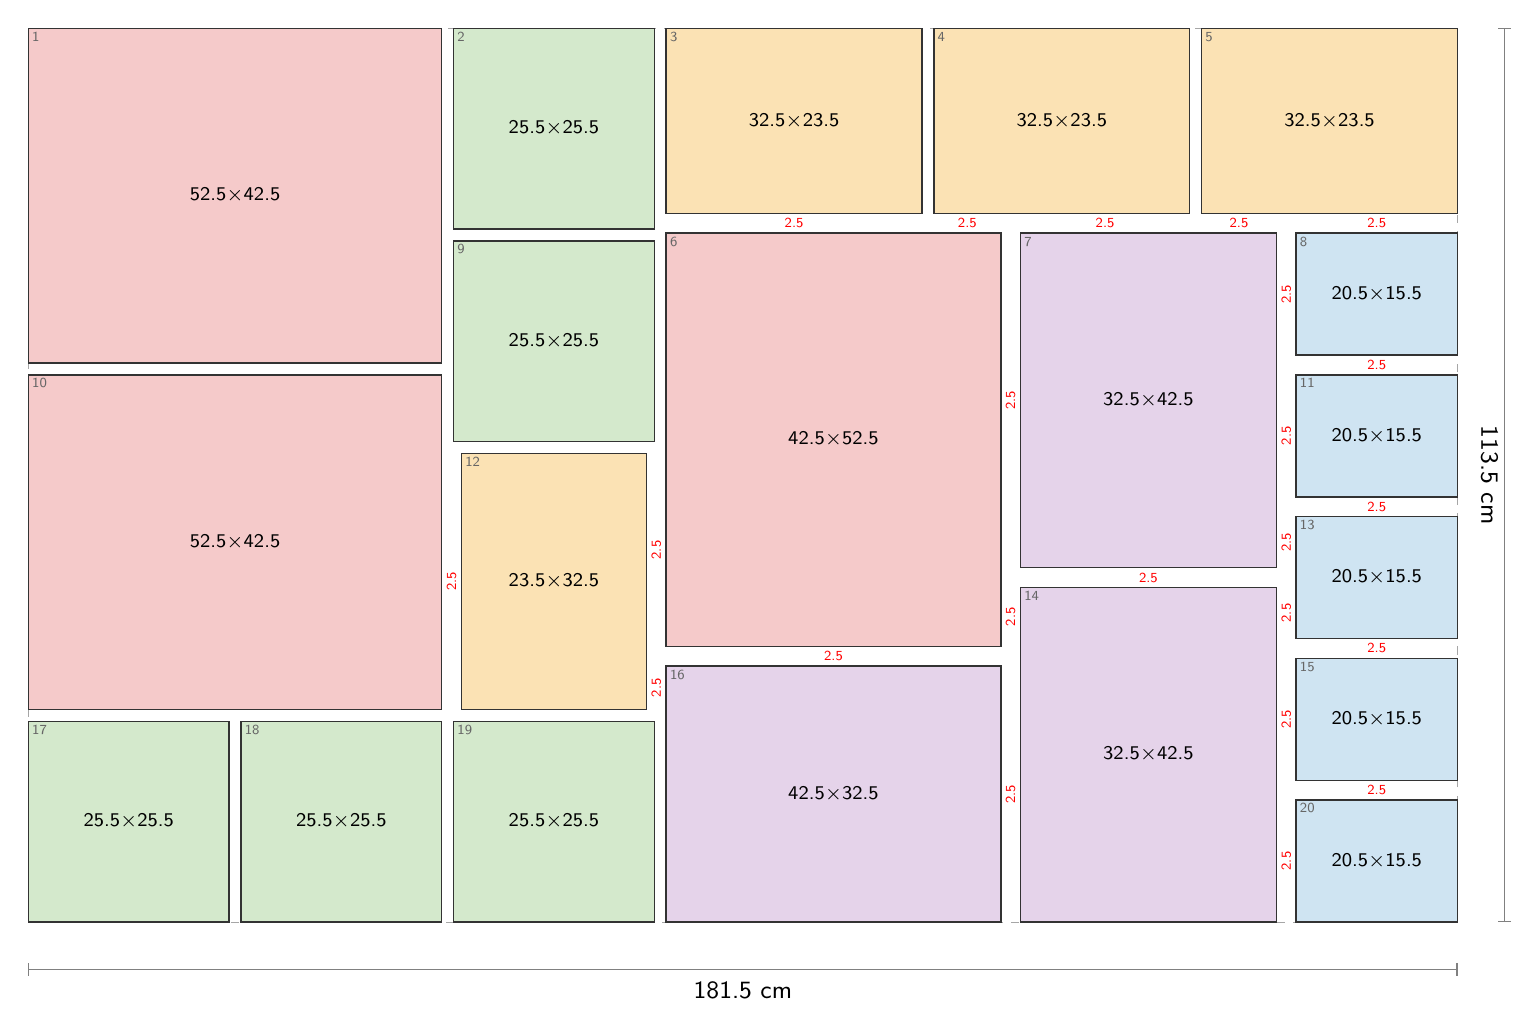
\begin{tikzpicture}[x=1mm, y=-1mm]
\draw[gray!70, dashed, line width=0.4pt] (0,0) rectangle (181.50,113.50);
\filldraw[fill=ft4, draw=black!80, line width=0.5pt] (0.00,0.00) rectangle (52.50,42.50);
\node[align=center, inner sep=0pt] at (26.25,21.25) {\scriptsize 52.5$\times$42.5};
\node[anchor=north west, inner sep=1.2pt, font=\tiny, text=black!60] at (0.00,0.00) {1};
\filldraw[fill=ft2, draw=black!80, line width=0.5pt] (54.00,0.00) rectangle (79.50,25.50);
\node[align=center, inner sep=0pt] at (66.75,12.75) {\scriptsize 25.5$\times$25.5};
\node[anchor=north west, inner sep=1.2pt, font=\tiny, text=black!60] at (54.00,0.00) {2};
\filldraw[fill=ft1, draw=black!80, line width=0.5pt] (81.00,0.00) rectangle (113.50,23.50);
\node[align=center, inner sep=0pt] at (97.25,11.75) {\scriptsize 32.5$\times$23.5};
\node[anchor=north west, inner sep=1.2pt, font=\tiny, text=black!60] at (81.00,0.00) {3};
\filldraw[fill=ft1, draw=black!80, line width=0.5pt] (115.00,0.00) rectangle (147.50,23.50);
\node[align=center, inner sep=0pt] at (131.25,11.75) {\scriptsize 32.5$\times$23.5};
\node[anchor=north west, inner sep=1.2pt, font=\tiny, text=black!60] at (115.00,0.00) {4};
\filldraw[fill=ft1, draw=black!80, line width=0.5pt] (149.00,0.00) rectangle (181.50,23.50);
\node[align=center, inner sep=0pt] at (165.25,11.75) {\scriptsize 32.5$\times$23.5};
\node[anchor=north west, inner sep=1.2pt, font=\tiny, text=black!60] at (149.00,0.00) {5};
\filldraw[fill=ft4, draw=black!80, line width=0.5pt] (81.00,26.00) rectangle (123.50,78.50);
\node[align=center, inner sep=0pt] at (102.25,52.25) {\scriptsize 42.5$\times$52.5};
\node[anchor=north west, inner sep=1.2pt, font=\tiny, text=black!60] at (81.00,26.00) {6};
\filldraw[fill=ft3, draw=black!80, line width=0.5pt] (126.00,26.00) rectangle (158.50,68.50);
\node[align=center, inner sep=0pt] at (142.25,47.25) {\scriptsize 32.5$\times$42.5};
\node[anchor=north west, inner sep=1.2pt, font=\tiny, text=black!60] at (126.00,26.00) {7};
\filldraw[fill=ft0, draw=black!80, line width=0.5pt] (161.00,26.00) rectangle (181.50,41.50);
\node[align=center, inner sep=0pt] at (171.25,33.75) {\scriptsize 20.5$\times$15.5};
\node[anchor=north west, inner sep=1.2pt, font=\tiny, text=black!60] at (161.00,26.00) {8};
\filldraw[fill=ft2, draw=black!80, line width=0.5pt] (54.00,27.00) rectangle (79.50,52.50);
\node[align=center, inner sep=0pt] at (66.75,39.75) {\scriptsize 25.5$\times$25.5};
\node[anchor=north west, inner sep=1.2pt, font=\tiny, text=black!60] at (54.00,27.00) {9};
\filldraw[fill=ft4, draw=black!80, line width=0.5pt] (0.00,44.00) rectangle (52.50,86.50);
\node[align=center, inner sep=0pt] at (26.25,65.25) {\scriptsize 52.5$\times$42.5};
\node[anchor=north west, inner sep=1.2pt, font=\tiny, text=black!60] at (0.00,44.00) {10};
\filldraw[fill=ft0, draw=black!80, line width=0.5pt] (161.00,44.00) rectangle (181.50,59.50);
\node[align=center, inner sep=0pt] at (171.25,51.75) {\scriptsize 20.5$\times$15.5};
\node[anchor=north west, inner sep=1.2pt, font=\tiny, text=black!60] at (161.00,44.00) {11};
\filldraw[fill=ft1, draw=black!80, line width=0.5pt] (55.00,54.00) rectangle (78.50,86.50);
\node[align=center, inner sep=0pt] at (66.75,70.25) {\scriptsize 23.5$\times$32.5};
\node[anchor=north west, inner sep=1.2pt, font=\tiny, text=black!60] at (55.00,54.00) {12};
\filldraw[fill=ft0, draw=black!80, line width=0.5pt] (161.00,62.00) rectangle (181.50,77.50);
\node[align=center, inner sep=0pt] at (171.25,69.75) {\scriptsize 20.5$\times$15.5};
\node[anchor=north west, inner sep=1.2pt, font=\tiny, text=black!60] at (161.00,62.00) {13};
\filldraw[fill=ft3, draw=black!80, line width=0.5pt] (126.00,71.00) rectangle (158.50,113.50);
\node[align=center, inner sep=0pt] at (142.25,92.25) {\scriptsize 32.5$\times$42.5};
\node[anchor=north west, inner sep=1.2pt, font=\tiny, text=black!60] at (126.00,71.00) {14};
\filldraw[fill=ft0, draw=black!80, line width=0.5pt] (161.00,80.00) rectangle (181.50,95.50);
\node[align=center, inner sep=0pt] at (171.25,87.75) {\scriptsize 20.5$\times$15.5};
\node[anchor=north west, inner sep=1.2pt, font=\tiny, text=black!60] at (161.00,80.00) {15};
\filldraw[fill=ft3, draw=black!80, line width=0.5pt] (81.00,81.00) rectangle (123.50,113.50);
\node[align=center, inner sep=0pt] at (102.25,97.25) {\scriptsize 42.5$\times$32.5};
\node[anchor=north west, inner sep=1.2pt, font=\tiny, text=black!60] at (81.00,81.00) {16};
\filldraw[fill=ft2, draw=black!80, line width=0.5pt] (0.00,88.00) rectangle (25.50,113.50);
\node[align=center, inner sep=0pt] at (12.75,100.75) {\scriptsize 25.5$\times$25.5};
\node[anchor=north west, inner sep=1.2pt, font=\tiny, text=black!60] at (0.00,88.00) {17};
\filldraw[fill=ft2, draw=black!80, line width=0.5pt] (27.00,88.00) rectangle (52.50,113.50);
\node[align=center, inner sep=0pt] at (39.75,100.75) {\scriptsize 25.5$\times$25.5};
\node[anchor=north west, inner sep=1.2pt, font=\tiny, text=black!60] at (27.00,88.00) {18};
\filldraw[fill=ft2, draw=black!80, line width=0.5pt] (54.00,88.00) rectangle (79.50,113.50);
\node[align=center, inner sep=0pt] at (66.75,100.75) {\scriptsize 25.5$\times$25.5};
\node[anchor=north west, inner sep=1.2pt, font=\tiny, text=black!60] at (54.00,88.00) {19};
\filldraw[fill=ft0, draw=black!80, line width=0.5pt] (161.00,98.00) rectangle (181.50,113.50);
\node[align=center, inner sep=0pt] at (171.25,105.75) {\scriptsize 20.5$\times$15.5};
\node[anchor=north west, inner sep=1.2pt, font=\tiny, text=black!60] at (161.00,98.00) {20};
\node[font=\tiny, text=red, fill=white, inner sep=0.3pt] at (97.25,24.75) {2.5};
\node[font=\tiny, text=red, fill=white, inner sep=0.3pt] at (119.25,24.75) {2.5};
\node[font=\tiny, text=red, fill=white, inner sep=0.3pt] at (136.75,24.75) {2.5};
\node[font=\tiny, text=red, fill=white, inner sep=0.3pt] at (153.75,24.75) {2.5};
\node[font=\tiny, text=red, fill=white, inner sep=0.3pt] at (171.25,24.75) {2.5};
\node[font=\tiny, text=red, fill=white, inner sep=0.3pt, rotate=90] at (124.75,47.25) {2.5};
\node[font=\tiny, text=red, fill=white, inner sep=0.3pt, rotate=90] at (124.75,74.75) {2.5};
\node[font=\tiny, text=red, fill=white, inner sep=0.3pt] at (102.25,79.75) {2.5};
\node[font=\tiny, text=red, fill=white, inner sep=0.3pt, rotate=90] at (159.75,33.75) {2.5};
\node[font=\tiny, text=red, fill=white, inner sep=0.3pt, rotate=90] at (159.75,51.75) {2.5};
\node[font=\tiny, text=red, fill=white, inner sep=0.3pt, rotate=90] at (159.75,65.25) {2.5};
\node[font=\tiny, text=red, fill=white, inner sep=0.3pt] at (142.25,69.75) {2.5};
\node[font=\tiny, text=red, fill=white, inner sep=0.3pt] at (171.25,42.75) {2.5};
\node[font=\tiny, text=red, fill=white, inner sep=0.3pt, rotate=90] at (53.75,70.25) {2.5};
\node[font=\tiny, text=red, fill=white, inner sep=0.3pt] at (171.25,60.75) {2.5};
\node[font=\tiny, text=red, fill=white, inner sep=0.3pt, rotate=90] at (79.75,66.25) {2.5};
\node[font=\tiny, text=red, fill=white, inner sep=0.3pt, rotate=90] at (79.75,83.75) {2.5};
\node[font=\tiny, text=red, fill=white, inner sep=0.3pt] at (171.25,78.75) {2.5};
\node[font=\tiny, text=red, fill=white, inner sep=0.3pt, rotate=90] at (159.75,74.25) {2.5};
\node[font=\tiny, text=red, fill=white, inner sep=0.3pt, rotate=90] at (159.75,87.75) {2.5};
\node[font=\tiny, text=red, fill=white, inner sep=0.3pt, rotate=90] at (159.75,105.75) {2.5};
\node[font=\tiny, text=red, fill=white, inner sep=0.3pt] at (171.25,96.75) {2.5};
\node[font=\tiny, text=red, fill=white, inner sep=0.3pt, rotate=90] at (124.75,97.25) {2.5};
\draw[Bar-Bar, gray] (0,119.50) -- (181.50,119.50) node[midway, below=1pt, font=\small, text=black] {181.5 cm};
\draw[Bar-Bar, gray] (187.50,0) -- (187.50,113.50) node[midway, right=1pt, font=\small, text=black, rotate=-90, anchor=north] {113.5 cm};
\end{tikzpicture}\\[4pt]
{\scriptsize Scale 1:10 (1 mm = 1 cm). Red numbers mark gaps that deviate from the nominal gap by more than 0.25 cm. Small grey numbers index the coordinate table.}
\end{minipage}\hfill
\begin{minipage}[t]{0.25\textwidth}\vspace{0pt}
\small
\begin{tabular}{@{}l l@{}}
\toprule
Outer size & 181.5 $\times$ 113.5 cm \\
Nominal gap & 1.5 cm \\
Actual gaps & 1.5 -- 2.5 cm \\
Max.\ deviation & 1.0 cm \\
Mean deviation & 0.59 cm \\
Border notches & none \\
Corners filled & 4 / 4 \\
Frames used & 20 of 28 \\
\bottomrule
\end{tabular}

\vspace{8pt}
\scriptsize
\begin{tabular}{@{}c l l r r@{}}
\toprule
 & outer w $\times$ h (cm) & & used & have \\
\midrule
\tikz[baseline=-0.6ex]\fill[ft0,draw=black!60] (0,0) rectangle (1.2ex,1.2ex); & 20.5$\times$15.5 & L & 5 & 9 \\
\tikz[baseline=-0.6ex]\fill[ft0,draw=black!60] (0,0) rectangle (1.2ex,1.2ex); & 15.5$\times$20.5 & P & 0 & 2 \\
\tikz[baseline=-0.6ex]\fill[ft3,draw=black!60] (0,0) rectangle (1.2ex,1.2ex); & 32.5$\times$42.5 & P & 2 & 2 \\
\tikz[baseline=-0.6ex]\fill[ft3,draw=black!60] (0,0) rectangle (1.2ex,1.2ex); & 42.5$\times$32.5 & L & 1 & 1 \\
\tikz[baseline=-0.6ex]\fill[ft1,draw=black!60] (0,0) rectangle (1.2ex,1.2ex); & 32.5$\times$23.5 & L & 3 & 5 \\
\tikz[baseline=-0.6ex]\fill[ft1,draw=black!60] (0,0) rectangle (1.2ex,1.2ex); & 23.5$\times$32.5 & P & 1 & 1 \\
\tikz[baseline=-0.6ex]\fill[ft2,draw=black!60] (0,0) rectangle (1.2ex,1.2ex); & 25.5$\times$25.5 &  & 5 & 5 \\
\tikz[baseline=-0.6ex]\fill[ft4,draw=black!60] (0,0) rectangle (1.2ex,1.2ex); & 42.5$\times$52.5 & P & 1 & 1 \\
\tikz[baseline=-0.6ex]\fill[ft4,draw=black!60] (0,0) rectangle (1.2ex,1.2ex); & 52.5$\times$42.5 & L & 2 & 2 \\
\bottomrule
\end{tabular}

\vspace{8pt}
{\bfseries Positions} (top-left corner, cm)\\[2pt]
\tiny
\begin{tabular}{@{}r l r r@{}}
\toprule
\# & frame w $\times$ h & x & y \\
\midrule
1 & 52.5 $\times$ 42.5 & 0.0 & 0.0 \\
2 & 25.5 $\times$ 25.5 & 54.0 & 0.0 \\
3 & 32.5 $\times$ 23.5 & 81.0 & 0.0 \\
4 & 32.5 $\times$ 23.5 & 115.0 & 0.0 \\
5 & 32.5 $\times$ 23.5 & 149.0 & 0.0 \\
6 & 42.5 $\times$ 52.5 & 81.0 & 26.0 \\
7 & 32.5 $\times$ 42.5 & 126.0 & 26.0 \\
8 & 20.5 $\times$ 15.5 & 161.0 & 26.0 \\
9 & 25.5 $\times$ 25.5 & 54.0 & 27.0 \\
10 & 52.5 $\times$ 42.5 & 0.0 & 44.0 \\
11 & 20.5 $\times$ 15.5 & 161.0 & 44.0 \\
12 & 23.5 $\times$ 32.5 & 55.0 & 54.0 \\
13 & 20.5 $\times$ 15.5 & 161.0 & 62.0 \\
14 & 32.5 $\times$ 42.5 & 126.0 & 71.0 \\
15 & 20.5 $\times$ 15.5 & 161.0 & 80.0 \\
16 & 42.5 $\times$ 32.5 & 81.0 & 81.0 \\
17 & 25.5 $\times$ 25.5 & 0.0 & 88.0 \\
18 & 25.5 $\times$ 25.5 & 27.0 & 88.0 \\
19 & 25.5 $\times$ 25.5 & 54.0 & 88.0 \\
20 & 20.5 $\times$ 15.5 & 161.0 & 98.0 \\
\bottomrule
\end{tabular}
\end{minipage}
\clearpage

\begin{minipage}[t]{0.74\textwidth}\vspace{0pt}
{\LARGE\bfseries Layout 2}\hspace{1.5em}{\large 182.0 $\times$ 129.0 cm \quad gap 4 cm \quad 24 frames}\\[8pt]
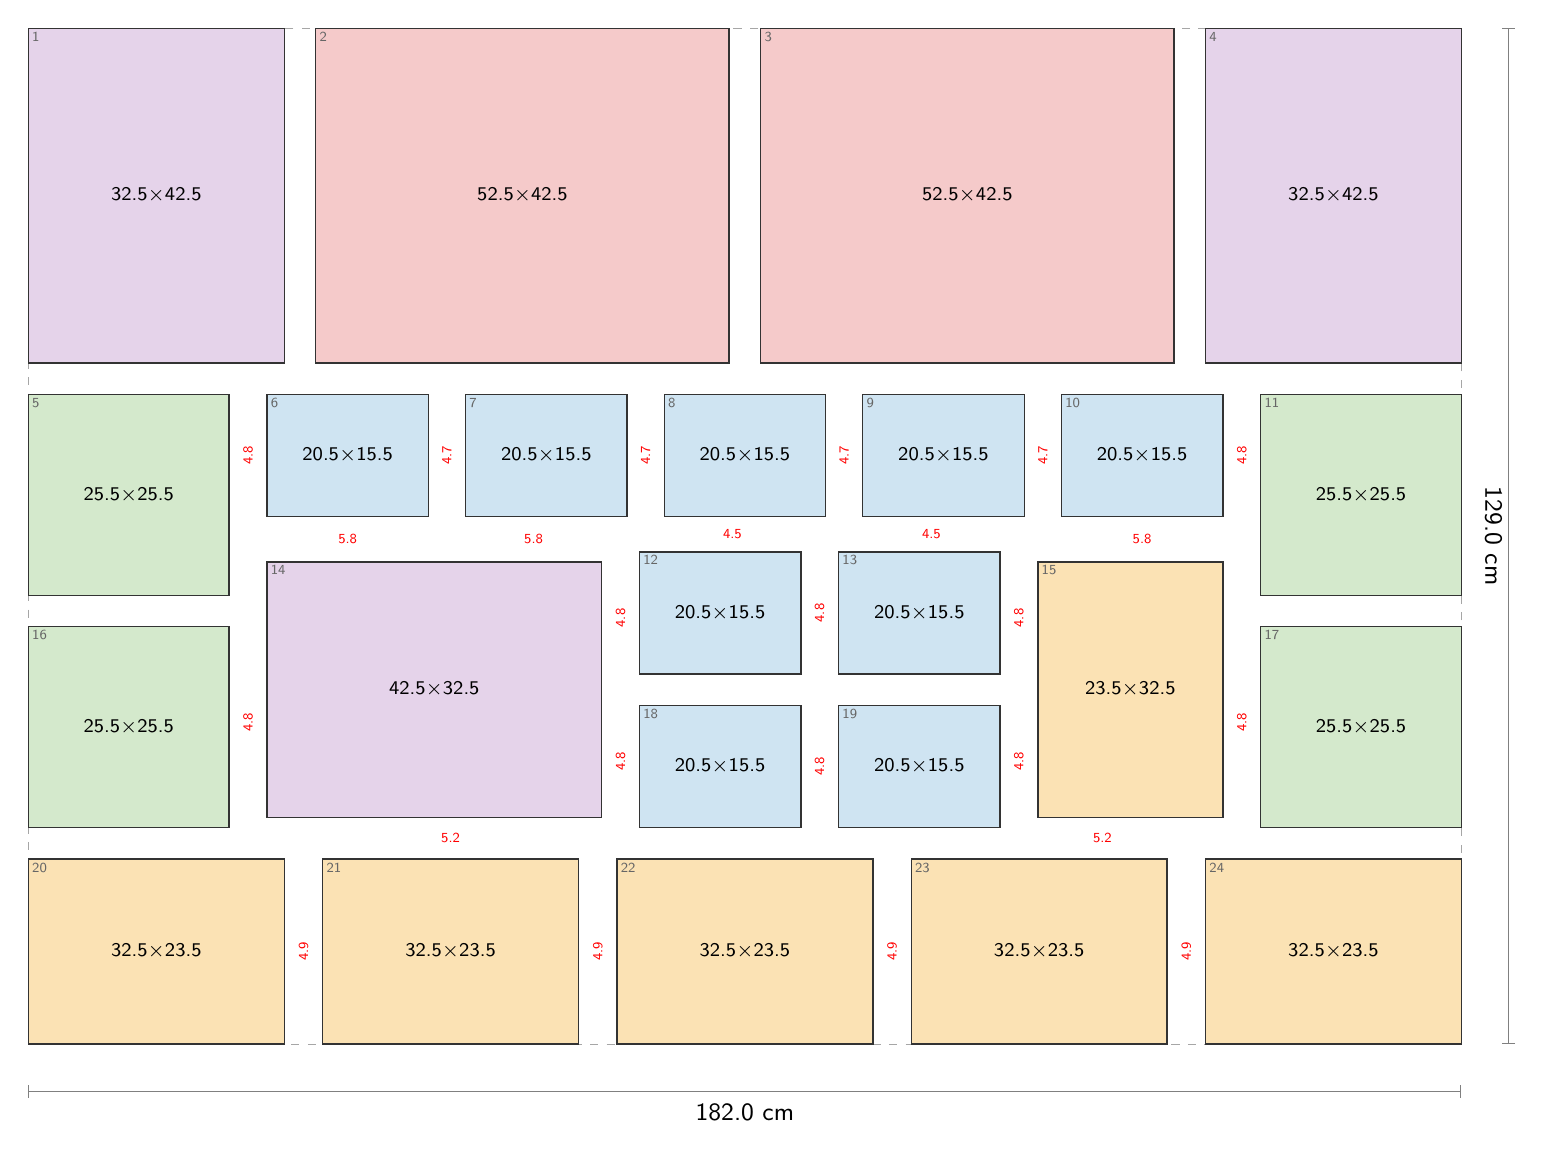
\begin{tikzpicture}[x=1mm, y=-1mm]
\draw[gray!70, dashed, line width=0.4pt] (0,0) rectangle (182.00,129.00);
\filldraw[fill=ft3, draw=black!80, line width=0.5pt] (0.00,0.00) rectangle (32.50,42.50);
\node[align=center, inner sep=0pt] at (16.25,21.25) {\scriptsize 32.5$\times$42.5};
\node[anchor=north west, inner sep=1.2pt, font=\tiny, text=black!60] at (0.00,0.00) {1};
\filldraw[fill=ft4, draw=black!80, line width=0.5pt] (36.50,0.00) rectangle (89.00,42.50);
\node[align=center, inner sep=0pt] at (62.75,21.25) {\scriptsize 52.5$\times$42.5};
\node[anchor=north west, inner sep=1.2pt, font=\tiny, text=black!60] at (36.50,0.00) {2};
\filldraw[fill=ft4, draw=black!80, line width=0.5pt] (93.00,0.00) rectangle (145.50,42.50);
\node[align=center, inner sep=0pt] at (119.25,21.25) {\scriptsize 52.5$\times$42.5};
\node[anchor=north west, inner sep=1.2pt, font=\tiny, text=black!60] at (93.00,0.00) {3};
\filldraw[fill=ft3, draw=black!80, line width=0.5pt] (149.50,0.00) rectangle (182.00,42.50);
\node[align=center, inner sep=0pt] at (165.75,21.25) {\scriptsize 32.5$\times$42.5};
\node[anchor=north west, inner sep=1.2pt, font=\tiny, text=black!60] at (149.50,0.00) {4};
\filldraw[fill=ft2, draw=black!80, line width=0.5pt] (0.00,46.50) rectangle (25.50,72.00);
\node[align=center, inner sep=0pt] at (12.75,59.25) {\scriptsize 25.5$\times$25.5};
\node[anchor=north west, inner sep=1.2pt, font=\tiny, text=black!60] at (0.00,46.50) {5};
\filldraw[fill=ft0, draw=black!80, line width=0.5pt] (30.30,46.50) rectangle (50.80,62.00);
\node[align=center, inner sep=0pt] at (40.55,54.25) {\scriptsize 20.5$\times$15.5};
\node[anchor=north west, inner sep=1.2pt, font=\tiny, text=black!60] at (30.30,46.50) {6};
\filldraw[fill=ft0, draw=black!80, line width=0.5pt] (55.52,46.50) rectangle (76.03,62.00);
\node[align=center, inner sep=0pt] at (65.78,54.25) {\scriptsize 20.5$\times$15.5};
\node[anchor=north west, inner sep=1.2pt, font=\tiny, text=black!60] at (55.52,46.50) {7};
\filldraw[fill=ft0, draw=black!80, line width=0.5pt] (80.75,46.50) rectangle (101.25,62.00);
\node[align=center, inner sep=0pt] at (91.00,54.25) {\scriptsize 20.5$\times$15.5};
\node[anchor=north west, inner sep=1.2pt, font=\tiny, text=black!60] at (80.75,46.50) {8};
\filldraw[fill=ft0, draw=black!80, line width=0.5pt] (105.97,46.50) rectangle (126.47,62.00);
\node[align=center, inner sep=0pt] at (116.22,54.25) {\scriptsize 20.5$\times$15.5};
\node[anchor=north west, inner sep=1.2pt, font=\tiny, text=black!60] at (105.97,46.50) {9};
\filldraw[fill=ft0, draw=black!80, line width=0.5pt] (131.20,46.50) rectangle (151.70,62.00);
\node[align=center, inner sep=0pt] at (141.45,54.25) {\scriptsize 20.5$\times$15.5};
\node[anchor=north west, inner sep=1.2pt, font=\tiny, text=black!60] at (131.20,46.50) {10};
\filldraw[fill=ft2, draw=black!80, line width=0.5pt] (156.50,46.50) rectangle (182.00,72.00);
\node[align=center, inner sep=0pt] at (169.25,59.25) {\scriptsize 25.5$\times$25.5};
\node[anchor=north west, inner sep=1.2pt, font=\tiny, text=black!60] at (156.50,46.50) {11};
\filldraw[fill=ft0, draw=black!80, line width=0.5pt] (77.60,66.50) rectangle (98.10,82.00);
\node[align=center, inner sep=0pt] at (87.85,74.25) {\scriptsize 20.5$\times$15.5};
\node[anchor=north west, inner sep=1.2pt, font=\tiny, text=black!60] at (77.60,66.50) {12};
\filldraw[fill=ft0, draw=black!80, line width=0.5pt] (102.90,66.50) rectangle (123.40,82.00);
\node[align=center, inner sep=0pt] at (113.15,74.25) {\scriptsize 20.5$\times$15.5};
\node[anchor=north west, inner sep=1.2pt, font=\tiny, text=black!60] at (102.90,66.50) {13};
\filldraw[fill=ft3, draw=black!80, line width=0.5pt] (30.30,67.75) rectangle (72.80,100.25);
\node[align=center, inner sep=0pt] at (51.55,84.00) {\scriptsize 42.5$\times$32.5};
\node[anchor=north west, inner sep=1.2pt, font=\tiny, text=black!60] at (30.30,67.75) {14};
\filldraw[fill=ft1, draw=black!80, line width=0.5pt] (128.20,67.75) rectangle (151.70,100.25);
\node[align=center, inner sep=0pt] at (139.95,84.00) {\scriptsize 23.5$\times$32.5};
\node[anchor=north west, inner sep=1.2pt, font=\tiny, text=black!60] at (128.20,67.75) {15};
\filldraw[fill=ft2, draw=black!80, line width=0.5pt] (0.00,76.00) rectangle (25.50,101.50);
\node[align=center, inner sep=0pt] at (12.75,88.75) {\scriptsize 25.5$\times$25.5};
\node[anchor=north west, inner sep=1.2pt, font=\tiny, text=black!60] at (0.00,76.00) {16};
\filldraw[fill=ft2, draw=black!80, line width=0.5pt] (156.50,76.00) rectangle (182.00,101.50);
\node[align=center, inner sep=0pt] at (169.25,88.75) {\scriptsize 25.5$\times$25.5};
\node[anchor=north west, inner sep=1.2pt, font=\tiny, text=black!60] at (156.50,76.00) {17};
\filldraw[fill=ft0, draw=black!80, line width=0.5pt] (77.60,86.00) rectangle (98.10,101.50);
\node[align=center, inner sep=0pt] at (87.85,93.75) {\scriptsize 20.5$\times$15.5};
\node[anchor=north west, inner sep=1.2pt, font=\tiny, text=black!60] at (77.60,86.00) {18};
\filldraw[fill=ft0, draw=black!80, line width=0.5pt] (102.90,86.00) rectangle (123.40,101.50);
\node[align=center, inner sep=0pt] at (113.15,93.75) {\scriptsize 20.5$\times$15.5};
\node[anchor=north west, inner sep=1.2pt, font=\tiny, text=black!60] at (102.90,86.00) {19};
\filldraw[fill=ft1, draw=black!80, line width=0.5pt] (0.00,105.50) rectangle (32.50,129.00);
\node[align=center, inner sep=0pt] at (16.25,117.25) {\scriptsize 32.5$\times$23.5};
\node[anchor=north west, inner sep=1.2pt, font=\tiny, text=black!60] at (0.00,105.50) {20};
\filldraw[fill=ft1, draw=black!80, line width=0.5pt] (37.38,105.50) rectangle (69.88,129.00);
\node[align=center, inner sep=0pt] at (53.62,117.25) {\scriptsize 32.5$\times$23.5};
\node[anchor=north west, inner sep=1.2pt, font=\tiny, text=black!60] at (37.38,105.50) {21};
\filldraw[fill=ft1, draw=black!80, line width=0.5pt] (74.75,105.50) rectangle (107.25,129.00);
\node[align=center, inner sep=0pt] at (91.00,117.25) {\scriptsize 32.5$\times$23.5};
\node[anchor=north west, inner sep=1.2pt, font=\tiny, text=black!60] at (74.75,105.50) {22};
\filldraw[fill=ft1, draw=black!80, line width=0.5pt] (112.12,105.50) rectangle (144.62,129.00);
\node[align=center, inner sep=0pt] at (128.38,117.25) {\scriptsize 32.5$\times$23.5};
\node[anchor=north west, inner sep=1.2pt, font=\tiny, text=black!60] at (112.12,105.50) {23};
\filldraw[fill=ft1, draw=black!80, line width=0.5pt] (149.50,105.50) rectangle (182.00,129.00);
\node[align=center, inner sep=0pt] at (165.75,117.25) {\scriptsize 32.5$\times$23.5};
\node[anchor=north west, inner sep=1.2pt, font=\tiny, text=black!60] at (149.50,105.50) {24};
\node[font=\tiny, text=red, fill=white, inner sep=0.3pt, rotate=90] at (27.90,54.25) {4.8};
\node[font=\tiny, text=red, fill=white, inner sep=0.3pt, rotate=90] at (53.16,54.25) {4.7};
\node[font=\tiny, text=red, fill=white, inner sep=0.3pt] at (40.55,64.88) {5.8};
\node[font=\tiny, text=red, fill=white, inner sep=0.3pt, rotate=90] at (78.39,54.25) {4.7};
\node[font=\tiny, text=red, fill=white, inner sep=0.3pt] at (64.16,64.88) {5.8};
\node[font=\tiny, text=red, fill=white, inner sep=0.3pt, rotate=90] at (103.61,54.25) {4.7};
\node[font=\tiny, text=red, fill=white, inner sep=0.3pt] at (89.42,64.25) {4.5};
\node[font=\tiny, text=red, fill=white, inner sep=0.3pt, rotate=90] at (128.84,54.25) {4.7};
\node[font=\tiny, text=red, fill=white, inner sep=0.3pt] at (114.69,64.25) {4.5};
\node[font=\tiny, text=red, fill=white, inner sep=0.3pt, rotate=90] at (154.10,54.25) {4.8};
\node[font=\tiny, text=red, fill=white, inner sep=0.3pt] at (141.45,64.88) {5.8};
\node[font=\tiny, text=red, fill=white, inner sep=0.3pt, rotate=90] at (100.50,74.25) {4.8};
\node[font=\tiny, text=red, fill=white, inner sep=0.3pt, rotate=90] at (125.80,74.88) {4.8};
\node[font=\tiny, text=red, fill=white, inner sep=0.3pt, rotate=90] at (75.20,74.88) {4.8};
\node[font=\tiny, text=red, fill=white, inner sep=0.3pt, rotate=90] at (75.20,93.12) {4.8};
\node[font=\tiny, text=red, fill=white, inner sep=0.3pt] at (53.62,102.88) {5.2};
\node[font=\tiny, text=red, fill=white, inner sep=0.3pt, rotate=90] at (154.10,88.12) {4.8};
\node[font=\tiny, text=red, fill=white, inner sep=0.3pt] at (136.41,102.88) {5.2};
\node[font=\tiny, text=red, fill=white, inner sep=0.3pt, rotate=90] at (27.90,88.12) {4.8};
\node[font=\tiny, text=red, fill=white, inner sep=0.3pt, rotate=90] at (100.50,93.75) {4.8};
\node[font=\tiny, text=red, fill=white, inner sep=0.3pt, rotate=90] at (125.80,93.12) {4.8};
\node[font=\tiny, text=red, fill=white, inner sep=0.3pt, rotate=90] at (34.94,117.25) {4.9};
\node[font=\tiny, text=red, fill=white, inner sep=0.3pt, rotate=90] at (72.31,117.25) {4.9};
\node[font=\tiny, text=red, fill=white, inner sep=0.3pt, rotate=90] at (109.69,117.25) {4.9};
\node[font=\tiny, text=red, fill=white, inner sep=0.3pt, rotate=90] at (147.06,117.25) {4.9};
\draw[Bar-Bar, gray] (0,135.00) -- (182.00,135.00) node[midway, below=1pt, font=\small, text=black] {182.0 cm};
\draw[Bar-Bar, gray] (188.00,0) -- (188.00,129.00) node[midway, right=1pt, font=\small, text=black, rotate=-90, anchor=north] {129.0 cm};
\end{tikzpicture}\\[4pt]
{\scriptsize Scale 1:10 (1 mm = 1 cm). Red numbers mark gaps that deviate from the nominal gap by more than 0.25 cm. Small grey numbers index the coordinate table.}
\end{minipage}\hfill
\begin{minipage}[t]{0.25\textwidth}\vspace{0pt}
\small
\begin{tabular}{@{}l l@{}}
\toprule
Outer size & 182.0 $\times$ 129.0 cm \\
Nominal gap & 4 cm \\
Actual gaps & 4.0 -- 5.8 cm \\
Max.\ deviation & 1.8 cm \\
Mean deviation & 0.53 cm \\
Border notches & none \\
Corners filled & 4 / 4 \\
Frames used & 24 of 28 \\
\bottomrule
\end{tabular}

\vspace{8pt}
\scriptsize
\begin{tabular}{@{}c l l r r@{}}
\toprule
 & outer w $\times$ h (cm) & & used & have \\
\midrule
\tikz[baseline=-0.6ex]\fill[ft0,draw=black!60] (0,0) rectangle (1.2ex,1.2ex); & 20.5$\times$15.5 & L & 9 & 9 \\
\tikz[baseline=-0.6ex]\fill[ft0,draw=black!60] (0,0) rectangle (1.2ex,1.2ex); & 15.5$\times$20.5 & P & 0 & 2 \\
\tikz[baseline=-0.6ex]\fill[ft3,draw=black!60] (0,0) rectangle (1.2ex,1.2ex); & 32.5$\times$42.5 & P & 2 & 2 \\
\tikz[baseline=-0.6ex]\fill[ft3,draw=black!60] (0,0) rectangle (1.2ex,1.2ex); & 42.5$\times$32.5 & L & 1 & 1 \\
\tikz[baseline=-0.6ex]\fill[ft1,draw=black!60] (0,0) rectangle (1.2ex,1.2ex); & 32.5$\times$23.5 & L & 5 & 5 \\
\tikz[baseline=-0.6ex]\fill[ft1,draw=black!60] (0,0) rectangle (1.2ex,1.2ex); & 23.5$\times$32.5 & P & 1 & 1 \\
\tikz[baseline=-0.6ex]\fill[ft2,draw=black!60] (0,0) rectangle (1.2ex,1.2ex); & 25.5$\times$25.5 &  & 4 & 5 \\
\tikz[baseline=-0.6ex]\fill[ft4,draw=black!60] (0,0) rectangle (1.2ex,1.2ex); & 42.5$\times$52.5 & P & 0 & 1 \\
\tikz[baseline=-0.6ex]\fill[ft4,draw=black!60] (0,0) rectangle (1.2ex,1.2ex); & 52.5$\times$42.5 & L & 2 & 2 \\
\bottomrule
\end{tabular}

\vspace{8pt}
{\bfseries Positions} (top-left corner, cm)\\[2pt]
\tiny
\begin{tabular}{@{}r l r r@{}}
\toprule
\# & frame w $\times$ h & x & y \\
\midrule
1 & 32.5 $\times$ 42.5 & 0.0 & 0.0 \\
2 & 52.5 $\times$ 42.5 & 36.5 & 0.0 \\
3 & 52.5 $\times$ 42.5 & 93.0 & 0.0 \\
4 & 32.5 $\times$ 42.5 & 149.5 & 0.0 \\
5 & 25.5 $\times$ 25.5 & 0.0 & 46.5 \\
6 & 20.5 $\times$ 15.5 & 30.3 & 46.5 \\
7 & 20.5 $\times$ 15.5 & 55.5 & 46.5 \\
8 & 20.5 $\times$ 15.5 & 80.8 & 46.5 \\
9 & 20.5 $\times$ 15.5 & 106.0 & 46.5 \\
10 & 20.5 $\times$ 15.5 & 131.2 & 46.5 \\
11 & 25.5 $\times$ 25.5 & 156.5 & 46.5 \\
12 & 20.5 $\times$ 15.5 & 77.6 & 66.5 \\
13 & 20.5 $\times$ 15.5 & 102.9 & 66.5 \\
14 & 42.5 $\times$ 32.5 & 30.3 & 67.8 \\
15 & 23.5 $\times$ 32.5 & 128.2 & 67.8 \\
16 & 25.5 $\times$ 25.5 & 0.0 & 76.0 \\
17 & 25.5 $\times$ 25.5 & 156.5 & 76.0 \\
18 & 20.5 $\times$ 15.5 & 77.6 & 86.0 \\
19 & 20.5 $\times$ 15.5 & 102.9 & 86.0 \\
20 & 32.5 $\times$ 23.5 & 0.0 & 105.5 \\
21 & 32.5 $\times$ 23.5 & 37.4 & 105.5 \\
22 & 32.5 $\times$ 23.5 & 74.8 & 105.5 \\
23 & 32.5 $\times$ 23.5 & 112.1 & 105.5 \\
24 & 32.5 $\times$ 23.5 & 149.5 & 105.5 \\
\bottomrule
\end{tabular}
\end{minipage}
\clearpage

\begin{minipage}[t]{0.74\textwidth}\vspace{0pt}
{\LARGE\bfseries Layout 3}\hspace{1.5em}{\large 184.0 $\times$ 115.0 cm \quad gap 2 cm \quad 23 frames}\\[8pt]
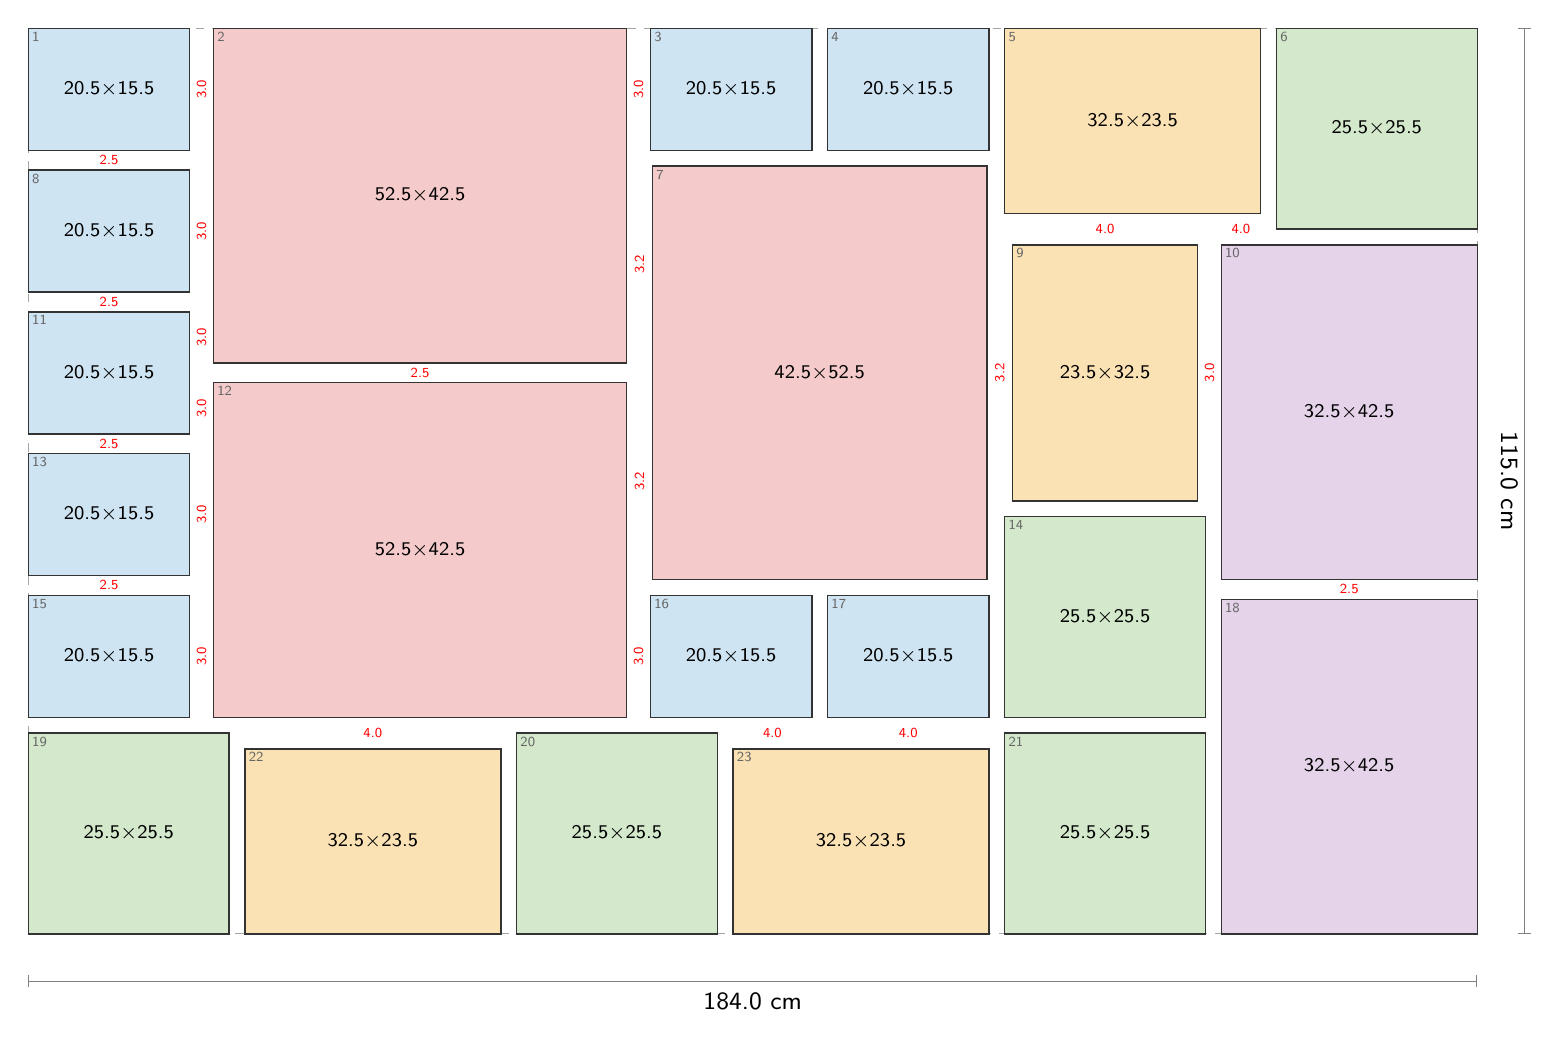
\begin{tikzpicture}[x=1mm, y=-1mm]
\draw[gray!70, dashed, line width=0.4pt] (0,0) rectangle (184.00,115.00);
\filldraw[fill=ft0, draw=black!80, line width=0.5pt] (0.00,0.00) rectangle (20.50,15.50);
\node[align=center, inner sep=0pt] at (10.25,7.75) {\scriptsize 20.5$\times$15.5};
\node[anchor=north west, inner sep=1.2pt, font=\tiny, text=black!60] at (0.00,0.00) {1};
\filldraw[fill=ft4, draw=black!80, line width=0.5pt] (23.50,0.00) rectangle (76.00,42.50);
\node[align=center, inner sep=0pt] at (49.75,21.25) {\scriptsize 52.5$\times$42.5};
\node[anchor=north west, inner sep=1.2pt, font=\tiny, text=black!60] at (23.50,0.00) {2};
\filldraw[fill=ft0, draw=black!80, line width=0.5pt] (79.00,0.00) rectangle (99.50,15.50);
\node[align=center, inner sep=0pt] at (89.25,7.75) {\scriptsize 20.5$\times$15.5};
\node[anchor=north west, inner sep=1.2pt, font=\tiny, text=black!60] at (79.00,0.00) {3};
\filldraw[fill=ft0, draw=black!80, line width=0.5pt] (101.50,0.00) rectangle (122.00,15.50);
\node[align=center, inner sep=0pt] at (111.75,7.75) {\scriptsize 20.5$\times$15.5};
\node[anchor=north west, inner sep=1.2pt, font=\tiny, text=black!60] at (101.50,0.00) {4};
\filldraw[fill=ft1, draw=black!80, line width=0.5pt] (124.00,0.00) rectangle (156.50,23.50);
\node[align=center, inner sep=0pt] at (140.25,11.75) {\scriptsize 32.5$\times$23.5};
\node[anchor=north west, inner sep=1.2pt, font=\tiny, text=black!60] at (124.00,0.00) {5};
\filldraw[fill=ft2, draw=black!80, line width=0.5pt] (158.50,0.00) rectangle (184.00,25.50);
\node[align=center, inner sep=0pt] at (171.25,12.75) {\scriptsize 25.5$\times$25.5};
\node[anchor=north west, inner sep=1.2pt, font=\tiny, text=black!60] at (158.50,0.00) {6};
\filldraw[fill=ft4, draw=black!80, line width=0.5pt] (79.25,17.50) rectangle (121.75,70.00);
\node[align=center, inner sep=0pt] at (100.50,43.75) {\scriptsize 42.5$\times$52.5};
\node[anchor=north west, inner sep=1.2pt, font=\tiny, text=black!60] at (79.25,17.50) {7};
\filldraw[fill=ft0, draw=black!80, line width=0.5pt] (0.00,18.00) rectangle (20.50,33.50);
\node[align=center, inner sep=0pt] at (10.25,25.75) {\scriptsize 20.5$\times$15.5};
\node[anchor=north west, inner sep=1.2pt, font=\tiny, text=black!60] at (0.00,18.00) {8};
\filldraw[fill=ft1, draw=black!80, line width=0.5pt] (125.00,27.50) rectangle (148.50,60.00);
\node[align=center, inner sep=0pt] at (136.75,43.75) {\scriptsize 23.5$\times$32.5};
\node[anchor=north west, inner sep=1.2pt, font=\tiny, text=black!60] at (125.00,27.50) {9};
\filldraw[fill=ft3, draw=black!80, line width=0.5pt] (151.50,27.50) rectangle (184.00,70.00);
\node[align=center, inner sep=0pt] at (167.75,48.75) {\scriptsize 32.5$\times$42.5};
\node[anchor=north west, inner sep=1.2pt, font=\tiny, text=black!60] at (151.50,27.50) {10};
\filldraw[fill=ft0, draw=black!80, line width=0.5pt] (0.00,36.00) rectangle (20.50,51.50);
\node[align=center, inner sep=0pt] at (10.25,43.75) {\scriptsize 20.5$\times$15.5};
\node[anchor=north west, inner sep=1.2pt, font=\tiny, text=black!60] at (0.00,36.00) {11};
\filldraw[fill=ft4, draw=black!80, line width=0.5pt] (23.50,45.00) rectangle (76.00,87.50);
\node[align=center, inner sep=0pt] at (49.75,66.25) {\scriptsize 52.5$\times$42.5};
\node[anchor=north west, inner sep=1.2pt, font=\tiny, text=black!60] at (23.50,45.00) {12};
\filldraw[fill=ft0, draw=black!80, line width=0.5pt] (0.00,54.00) rectangle (20.50,69.50);
\node[align=center, inner sep=0pt] at (10.25,61.75) {\scriptsize 20.5$\times$15.5};
\node[anchor=north west, inner sep=1.2pt, font=\tiny, text=black!60] at (0.00,54.00) {13};
\filldraw[fill=ft2, draw=black!80, line width=0.5pt] (124.00,62.00) rectangle (149.50,87.50);
\node[align=center, inner sep=0pt] at (136.75,74.75) {\scriptsize 25.5$\times$25.5};
\node[anchor=north west, inner sep=1.2pt, font=\tiny, text=black!60] at (124.00,62.00) {14};
\filldraw[fill=ft0, draw=black!80, line width=0.5pt] (0.00,72.00) rectangle (20.50,87.50);
\node[align=center, inner sep=0pt] at (10.25,79.75) {\scriptsize 20.5$\times$15.5};
\node[anchor=north west, inner sep=1.2pt, font=\tiny, text=black!60] at (0.00,72.00) {15};
\filldraw[fill=ft0, draw=black!80, line width=0.5pt] (79.00,72.00) rectangle (99.50,87.50);
\node[align=center, inner sep=0pt] at (89.25,79.75) {\scriptsize 20.5$\times$15.5};
\node[anchor=north west, inner sep=1.2pt, font=\tiny, text=black!60] at (79.00,72.00) {16};
\filldraw[fill=ft0, draw=black!80, line width=0.5pt] (101.50,72.00) rectangle (122.00,87.50);
\node[align=center, inner sep=0pt] at (111.75,79.75) {\scriptsize 20.5$\times$15.5};
\node[anchor=north west, inner sep=1.2pt, font=\tiny, text=black!60] at (101.50,72.00) {17};
\filldraw[fill=ft3, draw=black!80, line width=0.5pt] (151.50,72.50) rectangle (184.00,115.00);
\node[align=center, inner sep=0pt] at (167.75,93.75) {\scriptsize 32.5$\times$42.5};
\node[anchor=north west, inner sep=1.2pt, font=\tiny, text=black!60] at (151.50,72.50) {18};
\filldraw[fill=ft2, draw=black!80, line width=0.5pt] (0.00,89.50) rectangle (25.50,115.00);
\node[align=center, inner sep=0pt] at (12.75,102.25) {\scriptsize 25.5$\times$25.5};
\node[anchor=north west, inner sep=1.2pt, font=\tiny, text=black!60] at (0.00,89.50) {19};
\filldraw[fill=ft2, draw=black!80, line width=0.5pt] (62.00,89.50) rectangle (87.50,115.00);
\node[align=center, inner sep=0pt] at (74.75,102.25) {\scriptsize 25.5$\times$25.5};
\node[anchor=north west, inner sep=1.2pt, font=\tiny, text=black!60] at (62.00,89.50) {20};
\filldraw[fill=ft2, draw=black!80, line width=0.5pt] (124.00,89.50) rectangle (149.50,115.00);
\node[align=center, inner sep=0pt] at (136.75,102.25) {\scriptsize 25.5$\times$25.5};
\node[anchor=north west, inner sep=1.2pt, font=\tiny, text=black!60] at (124.00,89.50) {21};
\filldraw[fill=ft1, draw=black!80, line width=0.5pt] (27.50,91.50) rectangle (60.00,115.00);
\node[align=center, inner sep=0pt] at (43.75,103.25) {\scriptsize 32.5$\times$23.5};
\node[anchor=north west, inner sep=1.2pt, font=\tiny, text=black!60] at (27.50,91.50) {22};
\filldraw[fill=ft1, draw=black!80, line width=0.5pt] (89.50,91.50) rectangle (122.00,115.00);
\node[align=center, inner sep=0pt] at (105.75,103.25) {\scriptsize 32.5$\times$23.5};
\node[anchor=north west, inner sep=1.2pt, font=\tiny, text=black!60] at (89.50,91.50) {23};
\node[font=\tiny, text=red, fill=white, inner sep=0.3pt, rotate=90] at (22.00,7.75) {3.0};
\node[font=\tiny, text=red, fill=white, inner sep=0.3pt] at (10.25,16.75) {2.5};
\node[font=\tiny, text=red, fill=white, inner sep=0.3pt, rotate=90] at (77.50,7.75) {3.0};
\node[font=\tiny, text=red, fill=white, inner sep=0.3pt, rotate=90] at (77.62,30.00) {3.2};
\node[font=\tiny, text=red, fill=white, inner sep=0.3pt] at (49.75,43.75) {2.5};
\node[font=\tiny, text=red, fill=white, inner sep=0.3pt] at (136.75,25.50) {4.0};
\node[font=\tiny, text=red, fill=white, inner sep=0.3pt] at (154.00,25.50) {4.0};
\node[font=\tiny, text=red, fill=white, inner sep=0.3pt, rotate=90] at (123.38,43.75) {3.2};
\node[font=\tiny, text=red, fill=white, inner sep=0.3pt, rotate=90] at (22.00,25.75) {3.0};
\node[font=\tiny, text=red, fill=white, inner sep=0.3pt] at (10.25,34.75) {2.5};
\node[font=\tiny, text=red, fill=white, inner sep=0.3pt, rotate=90] at (150.00,43.75) {3.0};
\node[font=\tiny, text=red, fill=white, inner sep=0.3pt] at (167.75,71.25) {2.5};
\node[font=\tiny, text=red, fill=white, inner sep=0.3pt, rotate=90] at (22.00,39.25) {3.0};
\node[font=\tiny, text=red, fill=white, inner sep=0.3pt, rotate=90] at (22.00,48.25) {3.0};
\node[font=\tiny, text=red, fill=white, inner sep=0.3pt] at (10.25,52.75) {2.5};
\node[font=\tiny, text=red, fill=white, inner sep=0.3pt, rotate=90] at (77.62,57.50) {3.2};
\node[font=\tiny, text=red, fill=white, inner sep=0.3pt, rotate=90] at (77.50,79.75) {3.0};
\node[font=\tiny, text=red, fill=white, inner sep=0.3pt] at (43.75,89.50) {4.0};
\node[font=\tiny, text=red, fill=white, inner sep=0.3pt, rotate=90] at (22.00,61.75) {3.0};
\node[font=\tiny, text=red, fill=white, inner sep=0.3pt] at (10.25,70.75) {2.5};
\node[font=\tiny, text=red, fill=white, inner sep=0.3pt, rotate=90] at (22.00,79.75) {3.0};
\node[font=\tiny, text=red, fill=white, inner sep=0.3pt] at (94.50,89.50) {4.0};
\node[font=\tiny, text=red, fill=white, inner sep=0.3pt] at (111.75,89.50) {4.0};
\draw[Bar-Bar, gray] (0,121.00) -- (184.00,121.00) node[midway, below=1pt, font=\small, text=black] {184.0 cm};
\draw[Bar-Bar, gray] (190.00,0) -- (190.00,115.00) node[midway, right=1pt, font=\small, text=black, rotate=-90, anchor=north] {115.0 cm};
\end{tikzpicture}\\[4pt]
{\scriptsize Scale 1:10 (1 mm = 1 cm). Red numbers mark gaps that deviate from the nominal gap by more than 0.25 cm. Small grey numbers index the coordinate table.}
\end{minipage}\hfill
\begin{minipage}[t]{0.25\textwidth}\vspace{0pt}
\small
\begin{tabular}{@{}l l@{}}
\toprule
Outer size & 184.0 $\times$ 115.0 cm \\
Nominal gap & 2 cm \\
Actual gaps & 2.0 -- 4.0 cm \\
Max.\ deviation & 2.0 cm \\
Mean deviation & 0.56 cm \\
Border notches & none \\
Corners filled & 4 / 4 \\
Frames used & 23 of 28 \\
\bottomrule
\end{tabular}

\vspace{8pt}
\scriptsize
\begin{tabular}{@{}c l l r r@{}}
\toprule
 & outer w $\times$ h (cm) & & used & have \\
\midrule
\tikz[baseline=-0.6ex]\fill[ft0,draw=black!60] (0,0) rectangle (1.2ex,1.2ex); & 20.5$\times$15.5 & L & 9 & 9 \\
\tikz[baseline=-0.6ex]\fill[ft0,draw=black!60] (0,0) rectangle (1.2ex,1.2ex); & 15.5$\times$20.5 & P & 0 & 2 \\
\tikz[baseline=-0.6ex]\fill[ft3,draw=black!60] (0,0) rectangle (1.2ex,1.2ex); & 32.5$\times$42.5 & P & 2 & 2 \\
\tikz[baseline=-0.6ex]\fill[ft3,draw=black!60] (0,0) rectangle (1.2ex,1.2ex); & 42.5$\times$32.5 & L & 0 & 1 \\
\tikz[baseline=-0.6ex]\fill[ft1,draw=black!60] (0,0) rectangle (1.2ex,1.2ex); & 32.5$\times$23.5 & L & 3 & 5 \\
\tikz[baseline=-0.6ex]\fill[ft1,draw=black!60] (0,0) rectangle (1.2ex,1.2ex); & 23.5$\times$32.5 & P & 1 & 1 \\
\tikz[baseline=-0.6ex]\fill[ft2,draw=black!60] (0,0) rectangle (1.2ex,1.2ex); & 25.5$\times$25.5 &  & 5 & 5 \\
\tikz[baseline=-0.6ex]\fill[ft4,draw=black!60] (0,0) rectangle (1.2ex,1.2ex); & 42.5$\times$52.5 & P & 1 & 1 \\
\tikz[baseline=-0.6ex]\fill[ft4,draw=black!60] (0,0) rectangle (1.2ex,1.2ex); & 52.5$\times$42.5 & L & 2 & 2 \\
\bottomrule
\end{tabular}

\vspace{8pt}
{\bfseries Positions} (top-left corner, cm)\\[2pt]
\tiny
\begin{tabular}{@{}r l r r@{}}
\toprule
\# & frame w $\times$ h & x & y \\
\midrule
1 & 20.5 $\times$ 15.5 & 0.0 & 0.0 \\
2 & 52.5 $\times$ 42.5 & 23.5 & 0.0 \\
3 & 20.5 $\times$ 15.5 & 79.0 & 0.0 \\
4 & 20.5 $\times$ 15.5 & 101.5 & 0.0 \\
5 & 32.5 $\times$ 23.5 & 124.0 & 0.0 \\
6 & 25.5 $\times$ 25.5 & 158.5 & 0.0 \\
7 & 42.5 $\times$ 52.5 & 79.2 & 17.5 \\
8 & 20.5 $\times$ 15.5 & 0.0 & 18.0 \\
9 & 23.5 $\times$ 32.5 & 125.0 & 27.5 \\
10 & 32.5 $\times$ 42.5 & 151.5 & 27.5 \\
11 & 20.5 $\times$ 15.5 & 0.0 & 36.0 \\
12 & 52.5 $\times$ 42.5 & 23.5 & 45.0 \\
13 & 20.5 $\times$ 15.5 & 0.0 & 54.0 \\
14 & 25.5 $\times$ 25.5 & 124.0 & 62.0 \\
15 & 20.5 $\times$ 15.5 & 0.0 & 72.0 \\
16 & 20.5 $\times$ 15.5 & 79.0 & 72.0 \\
17 & 20.5 $\times$ 15.5 & 101.5 & 72.0 \\
18 & 32.5 $\times$ 42.5 & 151.5 & 72.5 \\
19 & 25.5 $\times$ 25.5 & 0.0 & 89.5 \\
20 & 25.5 $\times$ 25.5 & 62.0 & 89.5 \\
21 & 25.5 $\times$ 25.5 & 124.0 & 89.5 \\
22 & 32.5 $\times$ 23.5 & 27.5 & 91.5 \\
23 & 32.5 $\times$ 23.5 & 89.5 & 91.5 \\
\bottomrule
\end{tabular}
\end{minipage}
\clearpage

\begin{minipage}[t]{0.74\textwidth}\vspace{0pt}
{\LARGE\bfseries Layout 4}\hspace{1.5em}{\large 177.5 $\times$ 113.5 cm \quad gap 1.5 cm \quad 21 frames}\\[8pt]
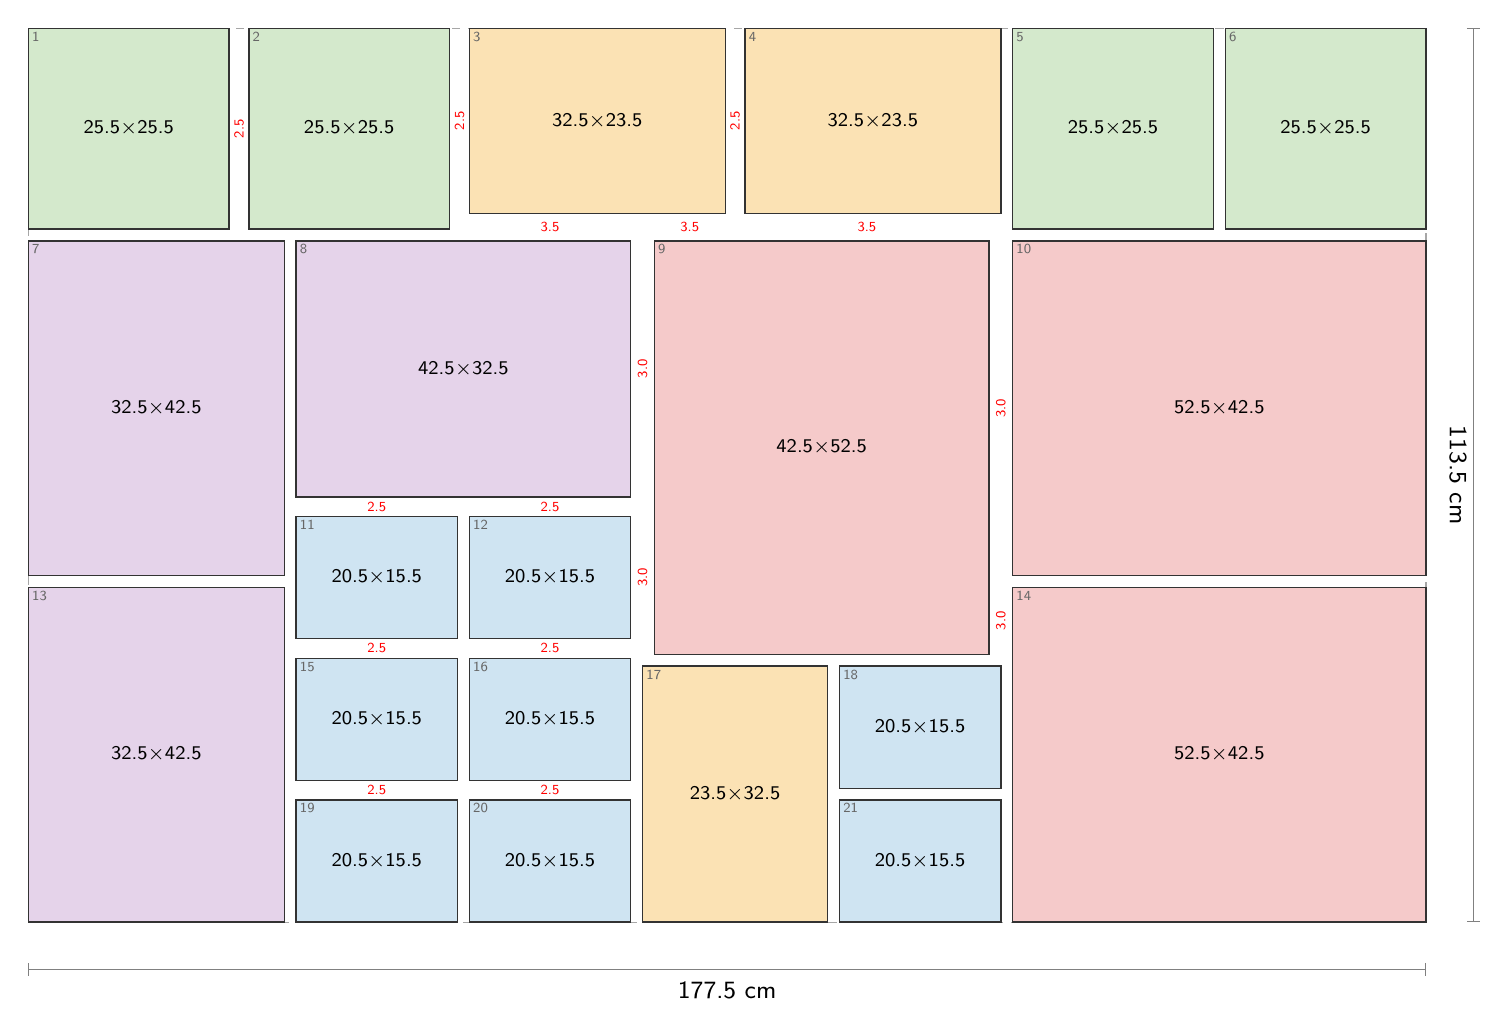
\begin{tikzpicture}[x=1mm, y=-1mm]
\draw[gray!70, dashed, line width=0.4pt] (0,0) rectangle (177.50,113.50);
\filldraw[fill=ft2, draw=black!80, line width=0.5pt] (0.00,0.00) rectangle (25.50,25.50);
\node[align=center, inner sep=0pt] at (12.75,12.75) {\scriptsize 25.5$\times$25.5};
\node[anchor=north west, inner sep=1.2pt, font=\tiny, text=black!60] at (0.00,0.00) {1};
\filldraw[fill=ft2, draw=black!80, line width=0.5pt] (28.00,0.00) rectangle (53.50,25.50);
\node[align=center, inner sep=0pt] at (40.75,12.75) {\scriptsize 25.5$\times$25.5};
\node[anchor=north west, inner sep=1.2pt, font=\tiny, text=black!60] at (28.00,0.00) {2};
\filldraw[fill=ft1, draw=black!80, line width=0.5pt] (56.00,0.00) rectangle (88.50,23.50);
\node[align=center, inner sep=0pt] at (72.25,11.75) {\scriptsize 32.5$\times$23.5};
\node[anchor=north west, inner sep=1.2pt, font=\tiny, text=black!60] at (56.00,0.00) {3};
\filldraw[fill=ft1, draw=black!80, line width=0.5pt] (91.00,0.00) rectangle (123.50,23.50);
\node[align=center, inner sep=0pt] at (107.25,11.75) {\scriptsize 32.5$\times$23.5};
\node[anchor=north west, inner sep=1.2pt, font=\tiny, text=black!60] at (91.00,0.00) {4};
\filldraw[fill=ft2, draw=black!80, line width=0.5pt] (125.00,0.00) rectangle (150.50,25.50);
\node[align=center, inner sep=0pt] at (137.75,12.75) {\scriptsize 25.5$\times$25.5};
\node[anchor=north west, inner sep=1.2pt, font=\tiny, text=black!60] at (125.00,0.00) {5};
\filldraw[fill=ft2, draw=black!80, line width=0.5pt] (152.00,0.00) rectangle (177.50,25.50);
\node[align=center, inner sep=0pt] at (164.75,12.75) {\scriptsize 25.5$\times$25.5};
\node[anchor=north west, inner sep=1.2pt, font=\tiny, text=black!60] at (152.00,0.00) {6};
\filldraw[fill=ft3, draw=black!80, line width=0.5pt] (0.00,27.00) rectangle (32.50,69.50);
\node[align=center, inner sep=0pt] at (16.25,48.25) {\scriptsize 32.5$\times$42.5};
\node[anchor=north west, inner sep=1.2pt, font=\tiny, text=black!60] at (0.00,27.00) {7};
\filldraw[fill=ft3, draw=black!80, line width=0.5pt] (34.00,27.00) rectangle (76.50,59.50);
\node[align=center, inner sep=0pt] at (55.25,43.25) {\scriptsize 42.5$\times$32.5};
\node[anchor=north west, inner sep=1.2pt, font=\tiny, text=black!60] at (34.00,27.00) {8};
\filldraw[fill=ft4, draw=black!80, line width=0.5pt] (79.50,27.00) rectangle (122.00,79.50);
\node[align=center, inner sep=0pt] at (100.75,53.25) {\scriptsize 42.5$\times$52.5};
\node[anchor=north west, inner sep=1.2pt, font=\tiny, text=black!60] at (79.50,27.00) {9};
\filldraw[fill=ft4, draw=black!80, line width=0.5pt] (125.00,27.00) rectangle (177.50,69.50);
\node[align=center, inner sep=0pt] at (151.25,48.25) {\scriptsize 52.5$\times$42.5};
\node[anchor=north west, inner sep=1.2pt, font=\tiny, text=black!60] at (125.00,27.00) {10};
\filldraw[fill=ft0, draw=black!80, line width=0.5pt] (34.00,62.00) rectangle (54.50,77.50);
\node[align=center, inner sep=0pt] at (44.25,69.75) {\scriptsize 20.5$\times$15.5};
\node[anchor=north west, inner sep=1.2pt, font=\tiny, text=black!60] at (34.00,62.00) {11};
\filldraw[fill=ft0, draw=black!80, line width=0.5pt] (56.00,62.00) rectangle (76.50,77.50);
\node[align=center, inner sep=0pt] at (66.25,69.75) {\scriptsize 20.5$\times$15.5};
\node[anchor=north west, inner sep=1.2pt, font=\tiny, text=black!60] at (56.00,62.00) {12};
\filldraw[fill=ft3, draw=black!80, line width=0.5pt] (0.00,71.00) rectangle (32.50,113.50);
\node[align=center, inner sep=0pt] at (16.25,92.25) {\scriptsize 32.5$\times$42.5};
\node[anchor=north west, inner sep=1.2pt, font=\tiny, text=black!60] at (0.00,71.00) {13};
\filldraw[fill=ft4, draw=black!80, line width=0.5pt] (125.00,71.00) rectangle (177.50,113.50);
\node[align=center, inner sep=0pt] at (151.25,92.25) {\scriptsize 52.5$\times$42.5};
\node[anchor=north west, inner sep=1.2pt, font=\tiny, text=black!60] at (125.00,71.00) {14};
\filldraw[fill=ft0, draw=black!80, line width=0.5pt] (34.00,80.00) rectangle (54.50,95.50);
\node[align=center, inner sep=0pt] at (44.25,87.75) {\scriptsize 20.5$\times$15.5};
\node[anchor=north west, inner sep=1.2pt, font=\tiny, text=black!60] at (34.00,80.00) {15};
\filldraw[fill=ft0, draw=black!80, line width=0.5pt] (56.00,80.00) rectangle (76.50,95.50);
\node[align=center, inner sep=0pt] at (66.25,87.75) {\scriptsize 20.5$\times$15.5};
\node[anchor=north west, inner sep=1.2pt, font=\tiny, text=black!60] at (56.00,80.00) {16};
\filldraw[fill=ft1, draw=black!80, line width=0.5pt] (78.00,81.00) rectangle (101.50,113.50);
\node[align=center, inner sep=0pt] at (89.75,97.25) {\scriptsize 23.5$\times$32.5};
\node[anchor=north west, inner sep=1.2pt, font=\tiny, text=black!60] at (78.00,81.00) {17};
\filldraw[fill=ft0, draw=black!80, line width=0.5pt] (103.00,81.00) rectangle (123.50,96.50);
\node[align=center, inner sep=0pt] at (113.25,88.75) {\scriptsize 20.5$\times$15.5};
\node[anchor=north west, inner sep=1.2pt, font=\tiny, text=black!60] at (103.00,81.00) {18};
\filldraw[fill=ft0, draw=black!80, line width=0.5pt] (34.00,98.00) rectangle (54.50,113.50);
\node[align=center, inner sep=0pt] at (44.25,105.75) {\scriptsize 20.5$\times$15.5};
\node[anchor=north west, inner sep=1.2pt, font=\tiny, text=black!60] at (34.00,98.00) {19};
\filldraw[fill=ft0, draw=black!80, line width=0.5pt] (56.00,98.00) rectangle (76.50,113.50);
\node[align=center, inner sep=0pt] at (66.25,105.75) {\scriptsize 20.5$\times$15.5};
\node[anchor=north west, inner sep=1.2pt, font=\tiny, text=black!60] at (56.00,98.00) {20};
\filldraw[fill=ft0, draw=black!80, line width=0.5pt] (103.00,98.00) rectangle (123.50,113.50);
\node[align=center, inner sep=0pt] at (113.25,105.75) {\scriptsize 20.5$\times$15.5};
\node[anchor=north west, inner sep=1.2pt, font=\tiny, text=black!60] at (103.00,98.00) {21};
\node[font=\tiny, text=red, fill=white, inner sep=0.3pt, rotate=90] at (26.75,12.75) {2.5};
\node[font=\tiny, text=red, fill=white, inner sep=0.3pt, rotate=90] at (54.75,11.75) {2.5};
\node[font=\tiny, text=red, fill=white, inner sep=0.3pt, rotate=90] at (89.75,11.75) {2.5};
\node[font=\tiny, text=red, fill=white, inner sep=0.3pt] at (66.25,25.25) {3.5};
\node[font=\tiny, text=red, fill=white, inner sep=0.3pt] at (84.00,25.25) {3.5};
\node[font=\tiny, text=red, fill=white, inner sep=0.3pt] at (106.50,25.25) {3.5};
\node[font=\tiny, text=red, fill=white, inner sep=0.3pt, rotate=90] at (78.00,43.25) {3.0};
\node[font=\tiny, text=red, fill=white, inner sep=0.3pt] at (44.25,60.75) {2.5};
\node[font=\tiny, text=red, fill=white, inner sep=0.3pt] at (66.25,60.75) {2.5};
\node[font=\tiny, text=red, fill=white, inner sep=0.3pt, rotate=90] at (123.50,48.25) {3.0};
\node[font=\tiny, text=red, fill=white, inner sep=0.3pt, rotate=90] at (123.50,75.25) {3.0};
\node[font=\tiny, text=red, fill=white, inner sep=0.3pt] at (44.25,78.75) {2.5};
\node[font=\tiny, text=red, fill=white, inner sep=0.3pt, rotate=90] at (78.00,69.75) {3.0};
\node[font=\tiny, text=red, fill=white, inner sep=0.3pt] at (66.25,78.75) {2.5};
\node[font=\tiny, text=red, fill=white, inner sep=0.3pt] at (44.25,96.75) {2.5};
\node[font=\tiny, text=red, fill=white, inner sep=0.3pt] at (66.25,96.75) {2.5};
\draw[Bar-Bar, gray] (0,119.50) -- (177.50,119.50) node[midway, below=1pt, font=\small, text=black] {177.5 cm};
\draw[Bar-Bar, gray] (183.50,0) -- (183.50,113.50) node[midway, right=1pt, font=\small, text=black, rotate=-90, anchor=north] {113.5 cm};
\end{tikzpicture}\\[4pt]
{\scriptsize Scale 1:10 (1 mm = 1 cm). Red numbers mark gaps that deviate from the nominal gap by more than 0.25 cm. Small grey numbers index the coordinate table.}
\end{minipage}\hfill
\begin{minipage}[t]{0.25\textwidth}\vspace{0pt}
\small
\begin{tabular}{@{}l l@{}}
\toprule
Outer size & 177.5 $\times$ 113.5 cm \\
Nominal gap & 1.5 cm \\
Actual gaps & 1.5 -- 3.5 cm \\
Max.\ deviation & 2.0 cm \\
Mean deviation & 0.51 cm \\
Border notches & none \\
Corners filled & 4 / 4 \\
Frames used & 21 of 28 \\
\bottomrule
\end{tabular}

\vspace{8pt}
\scriptsize
\begin{tabular}{@{}c l l r r@{}}
\toprule
 & outer w $\times$ h (cm) & & used & have \\
\midrule
\tikz[baseline=-0.6ex]\fill[ft0,draw=black!60] (0,0) rectangle (1.2ex,1.2ex); & 20.5$\times$15.5 & L & 8 & 9 \\
\tikz[baseline=-0.6ex]\fill[ft0,draw=black!60] (0,0) rectangle (1.2ex,1.2ex); & 15.5$\times$20.5 & P & 0 & 2 \\
\tikz[baseline=-0.6ex]\fill[ft3,draw=black!60] (0,0) rectangle (1.2ex,1.2ex); & 32.5$\times$42.5 & P & 2 & 2 \\
\tikz[baseline=-0.6ex]\fill[ft3,draw=black!60] (0,0) rectangle (1.2ex,1.2ex); & 42.5$\times$32.5 & L & 1 & 1 \\
\tikz[baseline=-0.6ex]\fill[ft1,draw=black!60] (0,0) rectangle (1.2ex,1.2ex); & 32.5$\times$23.5 & L & 2 & 5 \\
\tikz[baseline=-0.6ex]\fill[ft1,draw=black!60] (0,0) rectangle (1.2ex,1.2ex); & 23.5$\times$32.5 & P & 1 & 1 \\
\tikz[baseline=-0.6ex]\fill[ft2,draw=black!60] (0,0) rectangle (1.2ex,1.2ex); & 25.5$\times$25.5 &  & 4 & 5 \\
\tikz[baseline=-0.6ex]\fill[ft4,draw=black!60] (0,0) rectangle (1.2ex,1.2ex); & 42.5$\times$52.5 & P & 1 & 1 \\
\tikz[baseline=-0.6ex]\fill[ft4,draw=black!60] (0,0) rectangle (1.2ex,1.2ex); & 52.5$\times$42.5 & L & 2 & 2 \\
\bottomrule
\end{tabular}

\vspace{8pt}
{\bfseries Positions} (top-left corner, cm)\\[2pt]
\tiny
\begin{tabular}{@{}r l r r@{}}
\toprule
\# & frame w $\times$ h & x & y \\
\midrule
1 & 25.5 $\times$ 25.5 & 0.0 & 0.0 \\
2 & 25.5 $\times$ 25.5 & 28.0 & 0.0 \\
3 & 32.5 $\times$ 23.5 & 56.0 & 0.0 \\
4 & 32.5 $\times$ 23.5 & 91.0 & 0.0 \\
5 & 25.5 $\times$ 25.5 & 125.0 & 0.0 \\
6 & 25.5 $\times$ 25.5 & 152.0 & 0.0 \\
7 & 32.5 $\times$ 42.5 & 0.0 & 27.0 \\
8 & 42.5 $\times$ 32.5 & 34.0 & 27.0 \\
9 & 42.5 $\times$ 52.5 & 79.5 & 27.0 \\
10 & 52.5 $\times$ 42.5 & 125.0 & 27.0 \\
11 & 20.5 $\times$ 15.5 & 34.0 & 62.0 \\
12 & 20.5 $\times$ 15.5 & 56.0 & 62.0 \\
13 & 32.5 $\times$ 42.5 & 0.0 & 71.0 \\
14 & 52.5 $\times$ 42.5 & 125.0 & 71.0 \\
15 & 20.5 $\times$ 15.5 & 34.0 & 80.0 \\
16 & 20.5 $\times$ 15.5 & 56.0 & 80.0 \\
17 & 23.5 $\times$ 32.5 & 78.0 & 81.0 \\
18 & 20.5 $\times$ 15.5 & 103.0 & 81.0 \\
19 & 20.5 $\times$ 15.5 & 34.0 & 98.0 \\
20 & 20.5 $\times$ 15.5 & 56.0 & 98.0 \\
21 & 20.5 $\times$ 15.5 & 103.0 & 98.0 \\
\bottomrule
\end{tabular}
\end{minipage}
\clearpage

\begin{minipage}[t]{0.74\textwidth}\vspace{0pt}
{\LARGE\bfseries Layout 5}\hspace{1.5em}{\large 181.5 $\times$ 126.5 cm \quad gap 2.5 cm \quad 25 frames}\\[8pt]
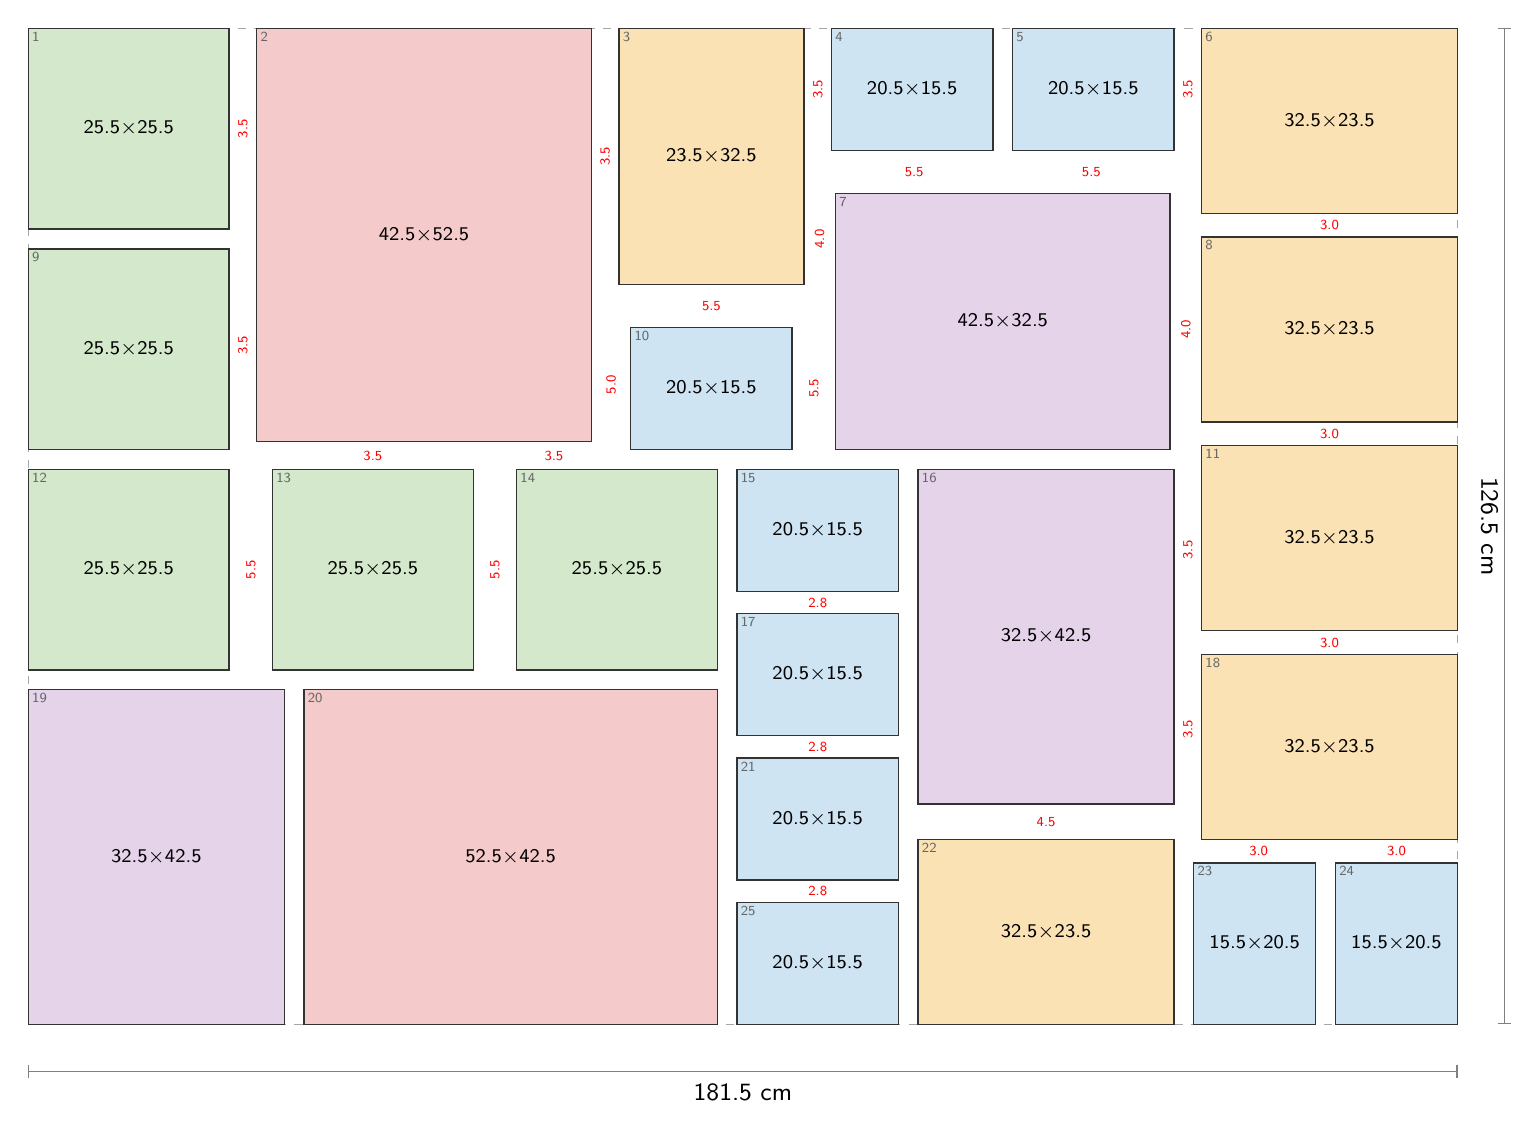
\begin{tikzpicture}[x=1mm, y=-1mm]
\draw[gray!70, dashed, line width=0.4pt] (0,0) rectangle (181.50,126.50);
\filldraw[fill=ft2, draw=black!80, line width=0.5pt] (0.00,0.00) rectangle (25.50,25.50);
\node[align=center, inner sep=0pt] at (12.75,12.75) {\scriptsize 25.5$\times$25.5};
\node[anchor=north west, inner sep=1.2pt, font=\tiny, text=black!60] at (0.00,0.00) {1};
\filldraw[fill=ft4, draw=black!80, line width=0.5pt] (29.00,0.00) rectangle (71.50,52.50);
\node[align=center, inner sep=0pt] at (50.25,26.25) {\scriptsize 42.5$\times$52.5};
\node[anchor=north west, inner sep=1.2pt, font=\tiny, text=black!60] at (29.00,0.00) {2};
\filldraw[fill=ft1, draw=black!80, line width=0.5pt] (75.00,0.00) rectangle (98.50,32.50);
\node[align=center, inner sep=0pt] at (86.75,16.25) {\scriptsize 23.5$\times$32.5};
\node[anchor=north west, inner sep=1.2pt, font=\tiny, text=black!60] at (75.00,0.00) {3};
\filldraw[fill=ft0, draw=black!80, line width=0.5pt] (102.00,0.00) rectangle (122.50,15.50);
\node[align=center, inner sep=0pt] at (112.25,7.75) {\scriptsize 20.5$\times$15.5};
\node[anchor=north west, inner sep=1.2pt, font=\tiny, text=black!60] at (102.00,0.00) {4};
\filldraw[fill=ft0, draw=black!80, line width=0.5pt] (125.00,0.00) rectangle (145.50,15.50);
\node[align=center, inner sep=0pt] at (135.25,7.75) {\scriptsize 20.5$\times$15.5};
\node[anchor=north west, inner sep=1.2pt, font=\tiny, text=black!60] at (125.00,0.00) {5};
\filldraw[fill=ft1, draw=black!80, line width=0.5pt] (149.00,0.00) rectangle (181.50,23.50);
\node[align=center, inner sep=0pt] at (165.25,11.75) {\scriptsize 32.5$\times$23.5};
\node[anchor=north west, inner sep=1.2pt, font=\tiny, text=black!60] at (149.00,0.00) {6};
\filldraw[fill=ft3, draw=black!80, line width=0.5pt] (102.50,21.00) rectangle (145.00,53.50);
\node[align=center, inner sep=0pt] at (123.75,37.25) {\scriptsize 42.5$\times$32.5};
\node[anchor=north west, inner sep=1.2pt, font=\tiny, text=black!60] at (102.50,21.00) {7};
\filldraw[fill=ft1, draw=black!80, line width=0.5pt] (149.00,26.50) rectangle (181.50,50.00);
\node[align=center, inner sep=0pt] at (165.25,38.25) {\scriptsize 32.5$\times$23.5};
\node[anchor=north west, inner sep=1.2pt, font=\tiny, text=black!60] at (149.00,26.50) {8};
\filldraw[fill=ft2, draw=black!80, line width=0.5pt] (0.00,28.00) rectangle (25.50,53.50);
\node[align=center, inner sep=0pt] at (12.75,40.75) {\scriptsize 25.5$\times$25.5};
\node[anchor=north west, inner sep=1.2pt, font=\tiny, text=black!60] at (0.00,28.00) {9};
\filldraw[fill=ft0, draw=black!80, line width=0.5pt] (76.50,38.00) rectangle (97.00,53.50);
\node[align=center, inner sep=0pt] at (86.75,45.75) {\scriptsize 20.5$\times$15.5};
\node[anchor=north west, inner sep=1.2pt, font=\tiny, text=black!60] at (76.50,38.00) {10};
\filldraw[fill=ft1, draw=black!80, line width=0.5pt] (149.00,53.00) rectangle (181.50,76.50);
\node[align=center, inner sep=0pt] at (165.25,64.75) {\scriptsize 32.5$\times$23.5};
\node[anchor=north west, inner sep=1.2pt, font=\tiny, text=black!60] at (149.00,53.00) {11};
\filldraw[fill=ft2, draw=black!80, line width=0.5pt] (0.00,56.00) rectangle (25.50,81.50);
\node[align=center, inner sep=0pt] at (12.75,68.75) {\scriptsize 25.5$\times$25.5};
\node[anchor=north west, inner sep=1.2pt, font=\tiny, text=black!60] at (0.00,56.00) {12};
\filldraw[fill=ft2, draw=black!80, line width=0.5pt] (31.00,56.00) rectangle (56.50,81.50);
\node[align=center, inner sep=0pt] at (43.75,68.75) {\scriptsize 25.5$\times$25.5};
\node[anchor=north west, inner sep=1.2pt, font=\tiny, text=black!60] at (31.00,56.00) {13};
\filldraw[fill=ft2, draw=black!80, line width=0.5pt] (62.00,56.00) rectangle (87.50,81.50);
\node[align=center, inner sep=0pt] at (74.75,68.75) {\scriptsize 25.5$\times$25.5};
\node[anchor=north west, inner sep=1.2pt, font=\tiny, text=black!60] at (62.00,56.00) {14};
\filldraw[fill=ft0, draw=black!80, line width=0.5pt] (90.00,56.00) rectangle (110.50,71.50);
\node[align=center, inner sep=0pt] at (100.25,63.75) {\scriptsize 20.5$\times$15.5};
\node[anchor=north west, inner sep=1.2pt, font=\tiny, text=black!60] at (90.00,56.00) {15};
\filldraw[fill=ft3, draw=black!80, line width=0.5pt] (113.00,56.00) rectangle (145.50,98.50);
\node[align=center, inner sep=0pt] at (129.25,77.25) {\scriptsize 32.5$\times$42.5};
\node[anchor=north west, inner sep=1.2pt, font=\tiny, text=black!60] at (113.00,56.00) {16};
\filldraw[fill=ft0, draw=black!80, line width=0.5pt] (90.00,74.33) rectangle (110.50,89.83);
\node[align=center, inner sep=0pt] at (100.25,82.08) {\scriptsize 20.5$\times$15.5};
\node[anchor=north west, inner sep=1.2pt, font=\tiny, text=black!60] at (90.00,74.33) {17};
\filldraw[fill=ft1, draw=black!80, line width=0.5pt] (149.00,79.50) rectangle (181.50,103.00);
\node[align=center, inner sep=0pt] at (165.25,91.25) {\scriptsize 32.5$\times$23.5};
\node[anchor=north west, inner sep=1.2pt, font=\tiny, text=black!60] at (149.00,79.50) {18};
\filldraw[fill=ft3, draw=black!80, line width=0.5pt] (0.00,84.00) rectangle (32.50,126.50);
\node[align=center, inner sep=0pt] at (16.25,105.25) {\scriptsize 32.5$\times$42.5};
\node[anchor=north west, inner sep=1.2pt, font=\tiny, text=black!60] at (0.00,84.00) {19};
\filldraw[fill=ft4, draw=black!80, line width=0.5pt] (35.00,84.00) rectangle (87.50,126.50);
\node[align=center, inner sep=0pt] at (61.25,105.25) {\scriptsize 52.5$\times$42.5};
\node[anchor=north west, inner sep=1.2pt, font=\tiny, text=black!60] at (35.00,84.00) {20};
\filldraw[fill=ft0, draw=black!80, line width=0.5pt] (90.00,92.67) rectangle (110.50,108.17);
\node[align=center, inner sep=0pt] at (100.25,100.42) {\scriptsize 20.5$\times$15.5};
\node[anchor=north west, inner sep=1.2pt, font=\tiny, text=black!60] at (90.00,92.67) {21};
\filldraw[fill=ft1, draw=black!80, line width=0.5pt] (113.00,103.00) rectangle (145.50,126.50);
\node[align=center, inner sep=0pt] at (129.25,114.75) {\scriptsize 32.5$\times$23.5};
\node[anchor=north west, inner sep=1.2pt, font=\tiny, text=black!60] at (113.00,103.00) {22};
\filldraw[fill=ft0, draw=black!80, line width=0.5pt] (148.00,106.00) rectangle (163.50,126.50);
\node[align=center, inner sep=0pt] at (155.75,116.25) {\scriptsize 15.5$\times$20.5};
\node[anchor=north west, inner sep=1.2pt, font=\tiny, text=black!60] at (148.00,106.00) {23};
\filldraw[fill=ft0, draw=black!80, line width=0.5pt] (166.00,106.00) rectangle (181.50,126.50);
\node[align=center, inner sep=0pt] at (173.75,116.25) {\scriptsize 15.5$\times$20.5};
\node[anchor=north west, inner sep=1.2pt, font=\tiny, text=black!60] at (166.00,106.00) {24};
\filldraw[fill=ft0, draw=black!80, line width=0.5pt] (90.00,111.00) rectangle (110.50,126.50);
\node[align=center, inner sep=0pt] at (100.25,118.75) {\scriptsize 20.5$\times$15.5};
\node[anchor=north west, inner sep=1.2pt, font=\tiny, text=black!60] at (90.00,111.00) {25};
\node[font=\tiny, text=red, fill=white, inner sep=0.3pt, rotate=90] at (27.25,12.75) {3.5};
\node[font=\tiny, text=red, fill=white, inner sep=0.3pt, rotate=90] at (73.25,16.25) {3.5};
\node[font=\tiny, text=red, fill=white, inner sep=0.3pt, rotate=90] at (74.00,45.25) {5.0};
\node[font=\tiny, text=red, fill=white, inner sep=0.3pt] at (43.75,54.25) {3.5};
\node[font=\tiny, text=red, fill=white, inner sep=0.3pt] at (66.75,54.25) {3.5};
\node[font=\tiny, text=red, fill=white, inner sep=0.3pt, rotate=90] at (100.25,7.75) {3.5};
\node[font=\tiny, text=red, fill=white, inner sep=0.3pt, rotate=90] at (100.50,26.75) {4.0};
\node[font=\tiny, text=red, fill=white, inner sep=0.3pt] at (86.75,35.25) {5.5};
\node[font=\tiny, text=red, fill=white, inner sep=0.3pt] at (112.50,18.25) {5.5};
\node[font=\tiny, text=red, fill=white, inner sep=0.3pt, rotate=90] at (147.25,7.75) {3.5};
\node[font=\tiny, text=red, fill=white, inner sep=0.3pt] at (135.00,18.25) {5.5};
\node[font=\tiny, text=red, fill=white, inner sep=0.3pt] at (165.25,25.00) {3.0};
\node[font=\tiny, text=red, fill=white, inner sep=0.3pt, rotate=90] at (147.00,38.25) {4.0};
\node[font=\tiny, text=red, fill=white, inner sep=0.3pt] at (165.25,51.50) {3.0};
\node[font=\tiny, text=red, fill=white, inner sep=0.3pt, rotate=90] at (27.25,40.25) {3.5};
\node[font=\tiny, text=red, fill=white, inner sep=0.3pt, rotate=90] at (99.75,45.75) {5.5};
\node[font=\tiny, text=red, fill=white, inner sep=0.3pt] at (165.25,78.00) {3.0};
\node[font=\tiny, text=red, fill=white, inner sep=0.3pt, rotate=90] at (28.25,68.75) {5.5};
\node[font=\tiny, text=red, fill=white, inner sep=0.3pt, rotate=90] at (59.25,68.75) {5.5};
\node[font=\tiny, text=red, fill=white, inner sep=0.3pt] at (100.25,72.92) {2.8};
\node[font=\tiny, text=red, fill=white, inner sep=0.3pt, rotate=90] at (147.25,66.25) {3.5};
\node[font=\tiny, text=red, fill=white, inner sep=0.3pt, rotate=90] at (147.25,89.00) {3.5};
\node[font=\tiny, text=red, fill=white, inner sep=0.3pt] at (129.25,100.75) {4.5};
\node[font=\tiny, text=red, fill=white, inner sep=0.3pt] at (100.25,91.25) {2.8};
\node[font=\tiny, text=red, fill=white, inner sep=0.3pt] at (156.25,104.50) {3.0};
\node[font=\tiny, text=red, fill=white, inner sep=0.3pt] at (173.75,104.50) {3.0};
\node[font=\tiny, text=red, fill=white, inner sep=0.3pt] at (100.25,109.58) {2.8};
\draw[Bar-Bar, gray] (0,132.50) -- (181.50,132.50) node[midway, below=1pt, font=\small, text=black] {181.5 cm};
\draw[Bar-Bar, gray] (187.50,0) -- (187.50,126.50) node[midway, right=1pt, font=\small, text=black, rotate=-90, anchor=north] {126.5 cm};
\end{tikzpicture}\\[4pt]
{\scriptsize Scale 1:10 (1 mm = 1 cm). Red numbers mark gaps that deviate from the nominal gap by more than 0.25 cm. Small grey numbers index the coordinate table.}
\end{minipage}\hfill
\begin{minipage}[t]{0.25\textwidth}\vspace{0pt}
\small
\begin{tabular}{@{}l l@{}}
\toprule
Outer size & 181.5 $\times$ 126.5 cm \\
Nominal gap & 2.5 cm \\
Actual gaps & 2.5 -- 5.5 cm \\
Max.\ deviation & 3.0 cm \\
Mean deviation & 0.76 cm \\
Border notches & none \\
Corners filled & 4 / 4 \\
Frames used & 25 of 28 \\
\bottomrule
\end{tabular}

\vspace{8pt}
\scriptsize
\begin{tabular}{@{}c l l r r@{}}
\toprule
 & outer w $\times$ h (cm) & & used & have \\
\midrule
\tikz[baseline=-0.6ex]\fill[ft0,draw=black!60] (0,0) rectangle (1.2ex,1.2ex); & 20.5$\times$15.5 & L & 7 & 9 \\
\tikz[baseline=-0.6ex]\fill[ft0,draw=black!60] (0,0) rectangle (1.2ex,1.2ex); & 15.5$\times$20.5 & P & 2 & 2 \\
\tikz[baseline=-0.6ex]\fill[ft3,draw=black!60] (0,0) rectangle (1.2ex,1.2ex); & 32.5$\times$42.5 & P & 2 & 2 \\
\tikz[baseline=-0.6ex]\fill[ft3,draw=black!60] (0,0) rectangle (1.2ex,1.2ex); & 42.5$\times$32.5 & L & 1 & 1 \\
\tikz[baseline=-0.6ex]\fill[ft1,draw=black!60] (0,0) rectangle (1.2ex,1.2ex); & 32.5$\times$23.5 & L & 5 & 5 \\
\tikz[baseline=-0.6ex]\fill[ft1,draw=black!60] (0,0) rectangle (1.2ex,1.2ex); & 23.5$\times$32.5 & P & 1 & 1 \\
\tikz[baseline=-0.6ex]\fill[ft2,draw=black!60] (0,0) rectangle (1.2ex,1.2ex); & 25.5$\times$25.5 &  & 5 & 5 \\
\tikz[baseline=-0.6ex]\fill[ft4,draw=black!60] (0,0) rectangle (1.2ex,1.2ex); & 42.5$\times$52.5 & P & 1 & 1 \\
\tikz[baseline=-0.6ex]\fill[ft4,draw=black!60] (0,0) rectangle (1.2ex,1.2ex); & 52.5$\times$42.5 & L & 1 & 2 \\
\bottomrule
\end{tabular}

\vspace{8pt}
{\bfseries Positions} (top-left corner, cm)\\[2pt]
\tiny
\begin{tabular}{@{}r l r r@{}}
\toprule
\# & frame w $\times$ h & x & y \\
\midrule
1 & 25.5 $\times$ 25.5 & 0.0 & 0.0 \\
2 & 42.5 $\times$ 52.5 & 29.0 & 0.0 \\
3 & 23.5 $\times$ 32.5 & 75.0 & 0.0 \\
4 & 20.5 $\times$ 15.5 & 102.0 & 0.0 \\
5 & 20.5 $\times$ 15.5 & 125.0 & 0.0 \\
6 & 32.5 $\times$ 23.5 & 149.0 & 0.0 \\
7 & 42.5 $\times$ 32.5 & 102.5 & 21.0 \\
8 & 32.5 $\times$ 23.5 & 149.0 & 26.5 \\
9 & 25.5 $\times$ 25.5 & 0.0 & 28.0 \\
10 & 20.5 $\times$ 15.5 & 76.5 & 38.0 \\
11 & 32.5 $\times$ 23.5 & 149.0 & 53.0 \\
12 & 25.5 $\times$ 25.5 & 0.0 & 56.0 \\
13 & 25.5 $\times$ 25.5 & 31.0 & 56.0 \\
14 & 25.5 $\times$ 25.5 & 62.0 & 56.0 \\
15 & 20.5 $\times$ 15.5 & 90.0 & 56.0 \\
16 & 32.5 $\times$ 42.5 & 113.0 & 56.0 \\
17 & 20.5 $\times$ 15.5 & 90.0 & 74.3 \\
18 & 32.5 $\times$ 23.5 & 149.0 & 79.5 \\
19 & 32.5 $\times$ 42.5 & 0.0 & 84.0 \\
20 & 52.5 $\times$ 42.5 & 35.0 & 84.0 \\
21 & 20.5 $\times$ 15.5 & 90.0 & 92.7 \\
22 & 32.5 $\times$ 23.5 & 113.0 & 103.0 \\
23 & 15.5 $\times$ 20.5 & 148.0 & 106.0 \\
24 & 15.5 $\times$ 20.5 & 166.0 & 106.0 \\
25 & 20.5 $\times$ 15.5 & 90.0 & 111.0 \\
\bottomrule
\end{tabular}
\end{minipage}
\clearpage

\begin{minipage}[t]{0.74\textwidth}\vspace{0pt}
{\LARGE\bfseries Layout 6}\hspace{1.5em}{\large 186.5 $\times$ 115.0 cm \quad gap 2 cm \quad 24 frames}\\[8pt]
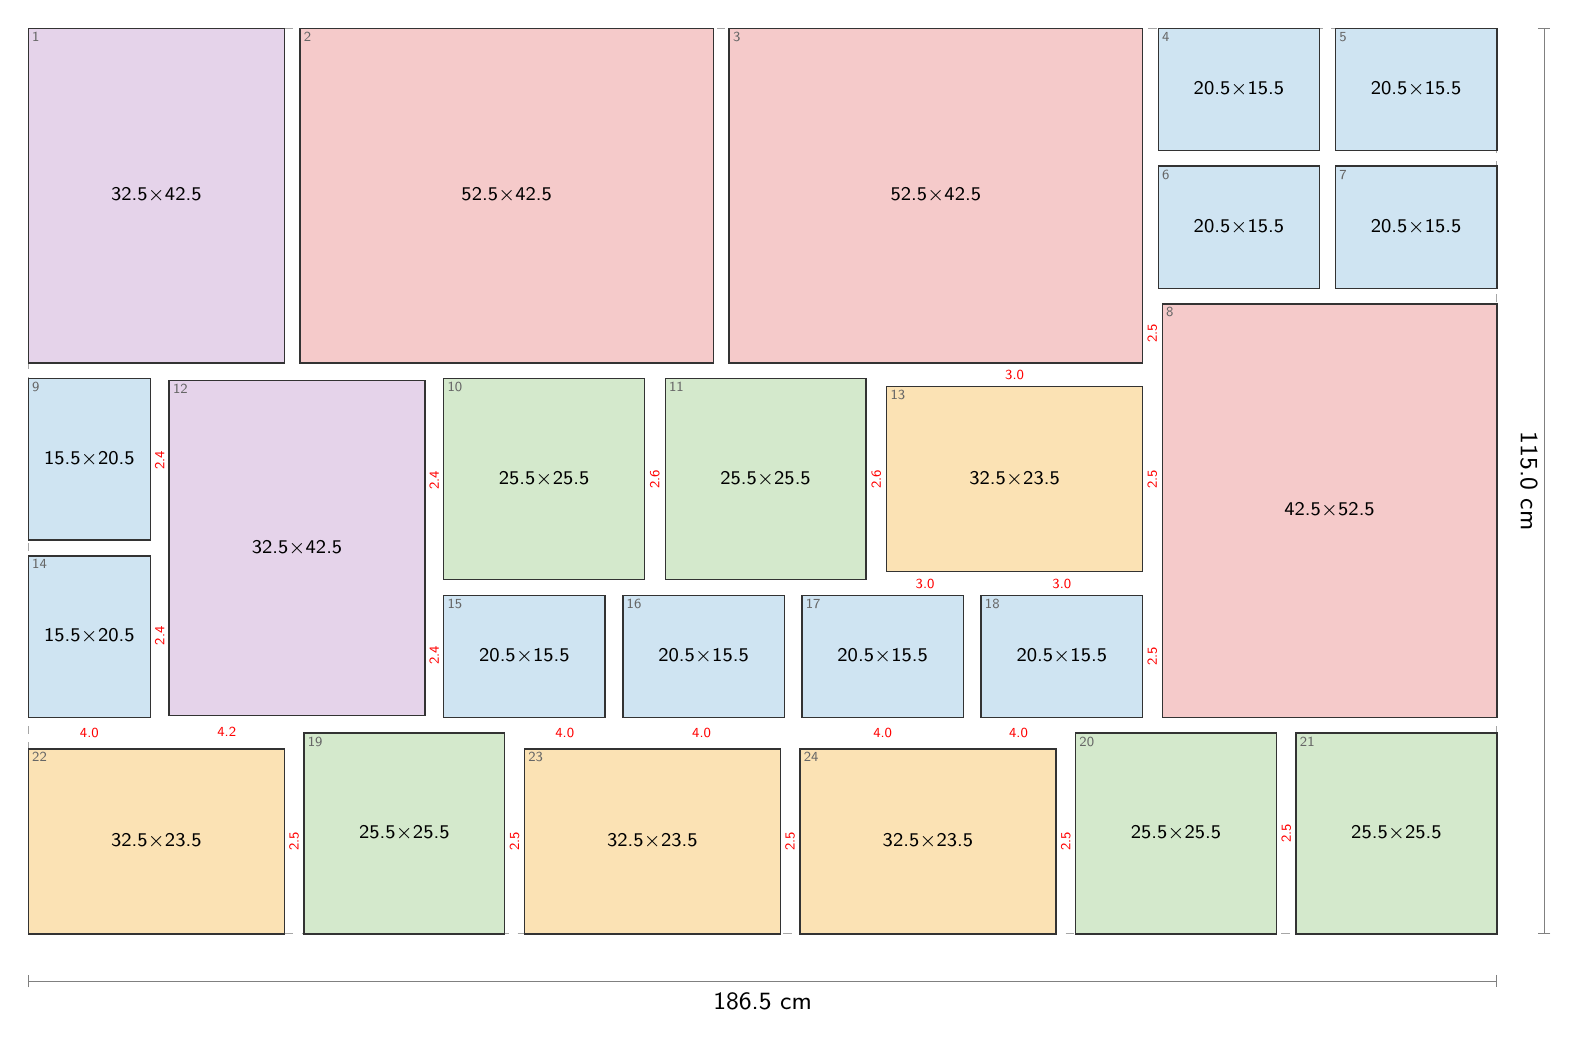
\begin{tikzpicture}[x=1mm, y=-1mm]
\draw[gray!70, dashed, line width=0.4pt] (0,0) rectangle (186.50,115.00);
\filldraw[fill=ft3, draw=black!80, line width=0.5pt] (0.00,0.00) rectangle (32.50,42.50);
\node[align=center, inner sep=0pt] at (16.25,21.25) {\scriptsize 32.5$\times$42.5};
\node[anchor=north west, inner sep=1.2pt, font=\tiny, text=black!60] at (0.00,0.00) {1};
\filldraw[fill=ft4, draw=black!80, line width=0.5pt] (34.50,0.00) rectangle (87.00,42.50);
\node[align=center, inner sep=0pt] at (60.75,21.25) {\scriptsize 52.5$\times$42.5};
\node[anchor=north west, inner sep=1.2pt, font=\tiny, text=black!60] at (34.50,0.00) {2};
\filldraw[fill=ft4, draw=black!80, line width=0.5pt] (89.00,0.00) rectangle (141.50,42.50);
\node[align=center, inner sep=0pt] at (115.25,21.25) {\scriptsize 52.5$\times$42.5};
\node[anchor=north west, inner sep=1.2pt, font=\tiny, text=black!60] at (89.00,0.00) {3};
\filldraw[fill=ft0, draw=black!80, line width=0.5pt] (143.50,0.00) rectangle (164.00,15.50);
\node[align=center, inner sep=0pt] at (153.75,7.75) {\scriptsize 20.5$\times$15.5};
\node[anchor=north west, inner sep=1.2pt, font=\tiny, text=black!60] at (143.50,0.00) {4};
\filldraw[fill=ft0, draw=black!80, line width=0.5pt] (166.00,0.00) rectangle (186.50,15.50);
\node[align=center, inner sep=0pt] at (176.25,7.75) {\scriptsize 20.5$\times$15.5};
\node[anchor=north west, inner sep=1.2pt, font=\tiny, text=black!60] at (166.00,0.00) {5};
\filldraw[fill=ft0, draw=black!80, line width=0.5pt] (143.50,17.50) rectangle (164.00,33.00);
\node[align=center, inner sep=0pt] at (153.75,25.25) {\scriptsize 20.5$\times$15.5};
\node[anchor=north west, inner sep=1.2pt, font=\tiny, text=black!60] at (143.50,17.50) {6};
\filldraw[fill=ft0, draw=black!80, line width=0.5pt] (166.00,17.50) rectangle (186.50,33.00);
\node[align=center, inner sep=0pt] at (176.25,25.25) {\scriptsize 20.5$\times$15.5};
\node[anchor=north west, inner sep=1.2pt, font=\tiny, text=black!60] at (166.00,17.50) {7};
\filldraw[fill=ft4, draw=black!80, line width=0.5pt] (144.00,35.00) rectangle (186.50,87.50);
\node[align=center, inner sep=0pt] at (165.25,61.25) {\scriptsize 42.5$\times$52.5};
\node[anchor=north west, inner sep=1.2pt, font=\tiny, text=black!60] at (144.00,35.00) {8};
\filldraw[fill=ft0, draw=black!80, line width=0.5pt] (0.00,44.50) rectangle (15.50,65.00);
\node[align=center, inner sep=0pt] at (7.75,54.75) {\scriptsize 15.5$\times$20.5};
\node[anchor=north west, inner sep=1.2pt, font=\tiny, text=black!60] at (0.00,44.50) {9};
\filldraw[fill=ft2, draw=black!80, line width=0.5pt] (52.75,44.50) rectangle (78.25,70.00);
\node[align=center, inner sep=0pt] at (65.50,57.25) {\scriptsize 25.5$\times$25.5};
\node[anchor=north west, inner sep=1.2pt, font=\tiny, text=black!60] at (52.75,44.50) {10};
\filldraw[fill=ft2, draw=black!80, line width=0.5pt] (80.88,44.50) rectangle (106.38,70.00);
\node[align=center, inner sep=0pt] at (93.62,57.25) {\scriptsize 25.5$\times$25.5};
\node[anchor=north west, inner sep=1.2pt, font=\tiny, text=black!60] at (80.88,44.50) {11};
\filldraw[fill=ft3, draw=black!80, line width=0.5pt] (17.88,44.75) rectangle (50.38,87.25);
\node[align=center, inner sep=0pt] at (34.12,66.00) {\scriptsize 32.5$\times$42.5};
\node[anchor=north west, inner sep=1.2pt, font=\tiny, text=black!60] at (17.88,44.75) {12};
\filldraw[fill=ft1, draw=black!80, line width=0.5pt] (109.00,45.50) rectangle (141.50,69.00);
\node[align=center, inner sep=0pt] at (125.25,57.25) {\scriptsize 32.5$\times$23.5};
\node[anchor=north west, inner sep=1.2pt, font=\tiny, text=black!60] at (109.00,45.50) {13};
\filldraw[fill=ft0, draw=black!80, line width=0.5pt] (0.00,67.00) rectangle (15.50,87.50);
\node[align=center, inner sep=0pt] at (7.75,77.25) {\scriptsize 15.5$\times$20.5};
\node[anchor=north west, inner sep=1.2pt, font=\tiny, text=black!60] at (0.00,67.00) {14};
\filldraw[fill=ft0, draw=black!80, line width=0.5pt] (52.75,72.00) rectangle (73.25,87.50);
\node[align=center, inner sep=0pt] at (63.00,79.75) {\scriptsize 20.5$\times$15.5};
\node[anchor=north west, inner sep=1.2pt, font=\tiny, text=black!60] at (52.75,72.00) {15};
\filldraw[fill=ft0, draw=black!80, line width=0.5pt] (75.50,72.00) rectangle (96.00,87.50);
\node[align=center, inner sep=0pt] at (85.75,79.75) {\scriptsize 20.5$\times$15.5};
\node[anchor=north west, inner sep=1.2pt, font=\tiny, text=black!60] at (75.50,72.00) {16};
\filldraw[fill=ft0, draw=black!80, line width=0.5pt] (98.25,72.00) rectangle (118.75,87.50);
\node[align=center, inner sep=0pt] at (108.50,79.75) {\scriptsize 20.5$\times$15.5};
\node[anchor=north west, inner sep=1.2pt, font=\tiny, text=black!60] at (98.25,72.00) {17};
\filldraw[fill=ft0, draw=black!80, line width=0.5pt] (121.00,72.00) rectangle (141.50,87.50);
\node[align=center, inner sep=0pt] at (131.25,79.75) {\scriptsize 20.5$\times$15.5};
\node[anchor=north west, inner sep=1.2pt, font=\tiny, text=black!60] at (121.00,72.00) {18};
\filldraw[fill=ft2, draw=black!80, line width=0.5pt] (35.00,89.50) rectangle (60.50,115.00);
\node[align=center, inner sep=0pt] at (47.75,102.25) {\scriptsize 25.5$\times$25.5};
\node[anchor=north west, inner sep=1.2pt, font=\tiny, text=black!60] at (35.00,89.50) {19};
\filldraw[fill=ft2, draw=black!80, line width=0.5pt] (133.00,89.50) rectangle (158.50,115.00);
\node[align=center, inner sep=0pt] at (145.75,102.25) {\scriptsize 25.5$\times$25.5};
\node[anchor=north west, inner sep=1.2pt, font=\tiny, text=black!60] at (133.00,89.50) {20};
\filldraw[fill=ft2, draw=black!80, line width=0.5pt] (161.00,89.50) rectangle (186.50,115.00);
\node[align=center, inner sep=0pt] at (173.75,102.25) {\scriptsize 25.5$\times$25.5};
\node[anchor=north west, inner sep=1.2pt, font=\tiny, text=black!60] at (161.00,89.50) {21};
\filldraw[fill=ft1, draw=black!80, line width=0.5pt] (0.00,91.50) rectangle (32.50,115.00);
\node[align=center, inner sep=0pt] at (16.25,103.25) {\scriptsize 32.5$\times$23.5};
\node[anchor=north west, inner sep=1.2pt, font=\tiny, text=black!60] at (0.00,91.50) {22};
\filldraw[fill=ft1, draw=black!80, line width=0.5pt] (63.00,91.50) rectangle (95.50,115.00);
\node[align=center, inner sep=0pt] at (79.25,103.25) {\scriptsize 32.5$\times$23.5};
\node[anchor=north west, inner sep=1.2pt, font=\tiny, text=black!60] at (63.00,91.50) {23};
\filldraw[fill=ft1, draw=black!80, line width=0.5pt] (98.00,91.50) rectangle (130.50,115.00);
\node[align=center, inner sep=0pt] at (114.25,103.25) {\scriptsize 32.5$\times$23.5};
\node[anchor=north west, inner sep=1.2pt, font=\tiny, text=black!60] at (98.00,91.50) {24};
\node[font=\tiny, text=red, fill=white, inner sep=0.3pt, rotate=90] at (142.75,38.75) {2.5};
\node[font=\tiny, text=red, fill=white, inner sep=0.3pt] at (125.25,44.00) {3.0};
\node[font=\tiny, text=red, fill=white, inner sep=0.3pt, rotate=90] at (16.69,54.88) {2.4};
\node[font=\tiny, text=red, fill=white, inner sep=0.3pt, rotate=90] at (79.56,57.25) {2.6};
\node[font=\tiny, text=red, fill=white, inner sep=0.3pt, rotate=90] at (107.69,57.25) {2.6};
\node[font=\tiny, text=red, fill=white, inner sep=0.3pt, rotate=90] at (51.56,57.38) {2.4};
\node[font=\tiny, text=red, fill=white, inner sep=0.3pt, rotate=90] at (51.56,79.62) {2.4};
\node[font=\tiny, text=red, fill=white, inner sep=0.3pt] at (25.19,89.38) {4.2};
\node[font=\tiny, text=red, fill=white, inner sep=0.3pt, rotate=90] at (142.75,57.25) {2.5};
\node[font=\tiny, text=red, fill=white, inner sep=0.3pt] at (113.88,70.50) {3.0};
\node[font=\tiny, text=red, fill=white, inner sep=0.3pt] at (131.25,70.50) {3.0};
\node[font=\tiny, text=red, fill=white, inner sep=0.3pt, rotate=90] at (16.69,77.12) {2.4};
\node[font=\tiny, text=red, fill=white, inner sep=0.3pt] at (7.75,89.50) {4.0};
\node[font=\tiny, text=red, fill=white, inner sep=0.3pt] at (68.12,89.50) {4.0};
\node[font=\tiny, text=red, fill=white, inner sep=0.3pt] at (85.50,89.50) {4.0};
\node[font=\tiny, text=red, fill=white, inner sep=0.3pt] at (108.50,89.50) {4.0};
\node[font=\tiny, text=red, fill=white, inner sep=0.3pt, rotate=90] at (142.75,79.75) {2.5};
\node[font=\tiny, text=red, fill=white, inner sep=0.3pt] at (125.75,89.50) {4.0};
\node[font=\tiny, text=red, fill=white, inner sep=0.3pt, rotate=90] at (61.75,103.25) {2.5};
\node[font=\tiny, text=red, fill=white, inner sep=0.3pt, rotate=90] at (159.75,102.25) {2.5};
\node[font=\tiny, text=red, fill=white, inner sep=0.3pt, rotate=90] at (33.75,103.25) {2.5};
\node[font=\tiny, text=red, fill=white, inner sep=0.3pt, rotate=90] at (96.75,103.25) {2.5};
\node[font=\tiny, text=red, fill=white, inner sep=0.3pt, rotate=90] at (131.75,103.25) {2.5};
\draw[Bar-Bar, gray] (0,121.00) -- (186.50,121.00) node[midway, below=1pt, font=\small, text=black] {186.5 cm};
\draw[Bar-Bar, gray] (192.50,0) -- (192.50,115.00) node[midway, right=1pt, font=\small, text=black, rotate=-90, anchor=north] {115.0 cm};
\end{tikzpicture}\\[4pt]
{\scriptsize Scale 1:10 (1 mm = 1 cm). Red numbers mark gaps that deviate from the nominal gap by more than 0.25 cm. Small grey numbers index the coordinate table.}
\end{minipage}\hfill
\begin{minipage}[t]{0.25\textwidth}\vspace{0pt}
\small
\begin{tabular}{@{}l l@{}}
\toprule
Outer size & 186.5 $\times$ 115.0 cm \\
Nominal gap & 2 cm \\
Actual gaps & 2.0 -- 4.2 cm \\
Max.\ deviation & 2.2 cm \\
Mean deviation & 0.46 cm \\
Border notches & left 4 cm \\
Corners filled & 4 / 4 \\
Frames used & 24 of 28 \\
\bottomrule
\end{tabular}

\vspace{8pt}
\scriptsize
\begin{tabular}{@{}c l l r r@{}}
\toprule
 & outer w $\times$ h (cm) & & used & have \\
\midrule
\tikz[baseline=-0.6ex]\fill[ft0,draw=black!60] (0,0) rectangle (1.2ex,1.2ex); & 20.5$\times$15.5 & L & 8 & 9 \\
\tikz[baseline=-0.6ex]\fill[ft0,draw=black!60] (0,0) rectangle (1.2ex,1.2ex); & 15.5$\times$20.5 & P & 2 & 2 \\
\tikz[baseline=-0.6ex]\fill[ft3,draw=black!60] (0,0) rectangle (1.2ex,1.2ex); & 32.5$\times$42.5 & P & 2 & 2 \\
\tikz[baseline=-0.6ex]\fill[ft3,draw=black!60] (0,0) rectangle (1.2ex,1.2ex); & 42.5$\times$32.5 & L & 0 & 1 \\
\tikz[baseline=-0.6ex]\fill[ft1,draw=black!60] (0,0) rectangle (1.2ex,1.2ex); & 32.5$\times$23.5 & L & 4 & 5 \\
\tikz[baseline=-0.6ex]\fill[ft1,draw=black!60] (0,0) rectangle (1.2ex,1.2ex); & 23.5$\times$32.5 & P & 0 & 1 \\
\tikz[baseline=-0.6ex]\fill[ft2,draw=black!60] (0,0) rectangle (1.2ex,1.2ex); & 25.5$\times$25.5 &  & 5 & 5 \\
\tikz[baseline=-0.6ex]\fill[ft4,draw=black!60] (0,0) rectangle (1.2ex,1.2ex); & 42.5$\times$52.5 & P & 1 & 1 \\
\tikz[baseline=-0.6ex]\fill[ft4,draw=black!60] (0,0) rectangle (1.2ex,1.2ex); & 52.5$\times$42.5 & L & 2 & 2 \\
\bottomrule
\end{tabular}

\vspace{8pt}
{\bfseries Positions} (top-left corner, cm)\\[2pt]
\tiny
\begin{tabular}{@{}r l r r@{}}
\toprule
\# & frame w $\times$ h & x & y \\
\midrule
1 & 32.5 $\times$ 42.5 & 0.0 & 0.0 \\
2 & 52.5 $\times$ 42.5 & 34.5 & 0.0 \\
3 & 52.5 $\times$ 42.5 & 89.0 & 0.0 \\
4 & 20.5 $\times$ 15.5 & 143.5 & 0.0 \\
5 & 20.5 $\times$ 15.5 & 166.0 & 0.0 \\
6 & 20.5 $\times$ 15.5 & 143.5 & 17.5 \\
7 & 20.5 $\times$ 15.5 & 166.0 & 17.5 \\
8 & 42.5 $\times$ 52.5 & 144.0 & 35.0 \\
9 & 15.5 $\times$ 20.5 & 0.0 & 44.5 \\
10 & 25.5 $\times$ 25.5 & 52.8 & 44.5 \\
11 & 25.5 $\times$ 25.5 & 80.9 & 44.5 \\
12 & 32.5 $\times$ 42.5 & 17.9 & 44.8 \\
13 & 32.5 $\times$ 23.5 & 109.0 & 45.5 \\
14 & 15.5 $\times$ 20.5 & 0.0 & 67.0 \\
15 & 20.5 $\times$ 15.5 & 52.8 & 72.0 \\
16 & 20.5 $\times$ 15.5 & 75.5 & 72.0 \\
17 & 20.5 $\times$ 15.5 & 98.2 & 72.0 \\
18 & 20.5 $\times$ 15.5 & 121.0 & 72.0 \\
19 & 25.5 $\times$ 25.5 & 35.0 & 89.5 \\
20 & 25.5 $\times$ 25.5 & 133.0 & 89.5 \\
21 & 25.5 $\times$ 25.5 & 161.0 & 89.5 \\
22 & 32.5 $\times$ 23.5 & 0.0 & 91.5 \\
23 & 32.5 $\times$ 23.5 & 63.0 & 91.5 \\
24 & 32.5 $\times$ 23.5 & 98.0 & 91.5 \\
\bottomrule
\end{tabular}
\end{minipage}
\clearpage

\begin{minipage}[t]{0.74\textwidth}\vspace{0pt}
{\LARGE\bfseries Layout 7}\hspace{1.5em}{\large 180.5 $\times$ 128.5 cm \quad gap 3.5 cm \quad 24 frames}\\[8pt]
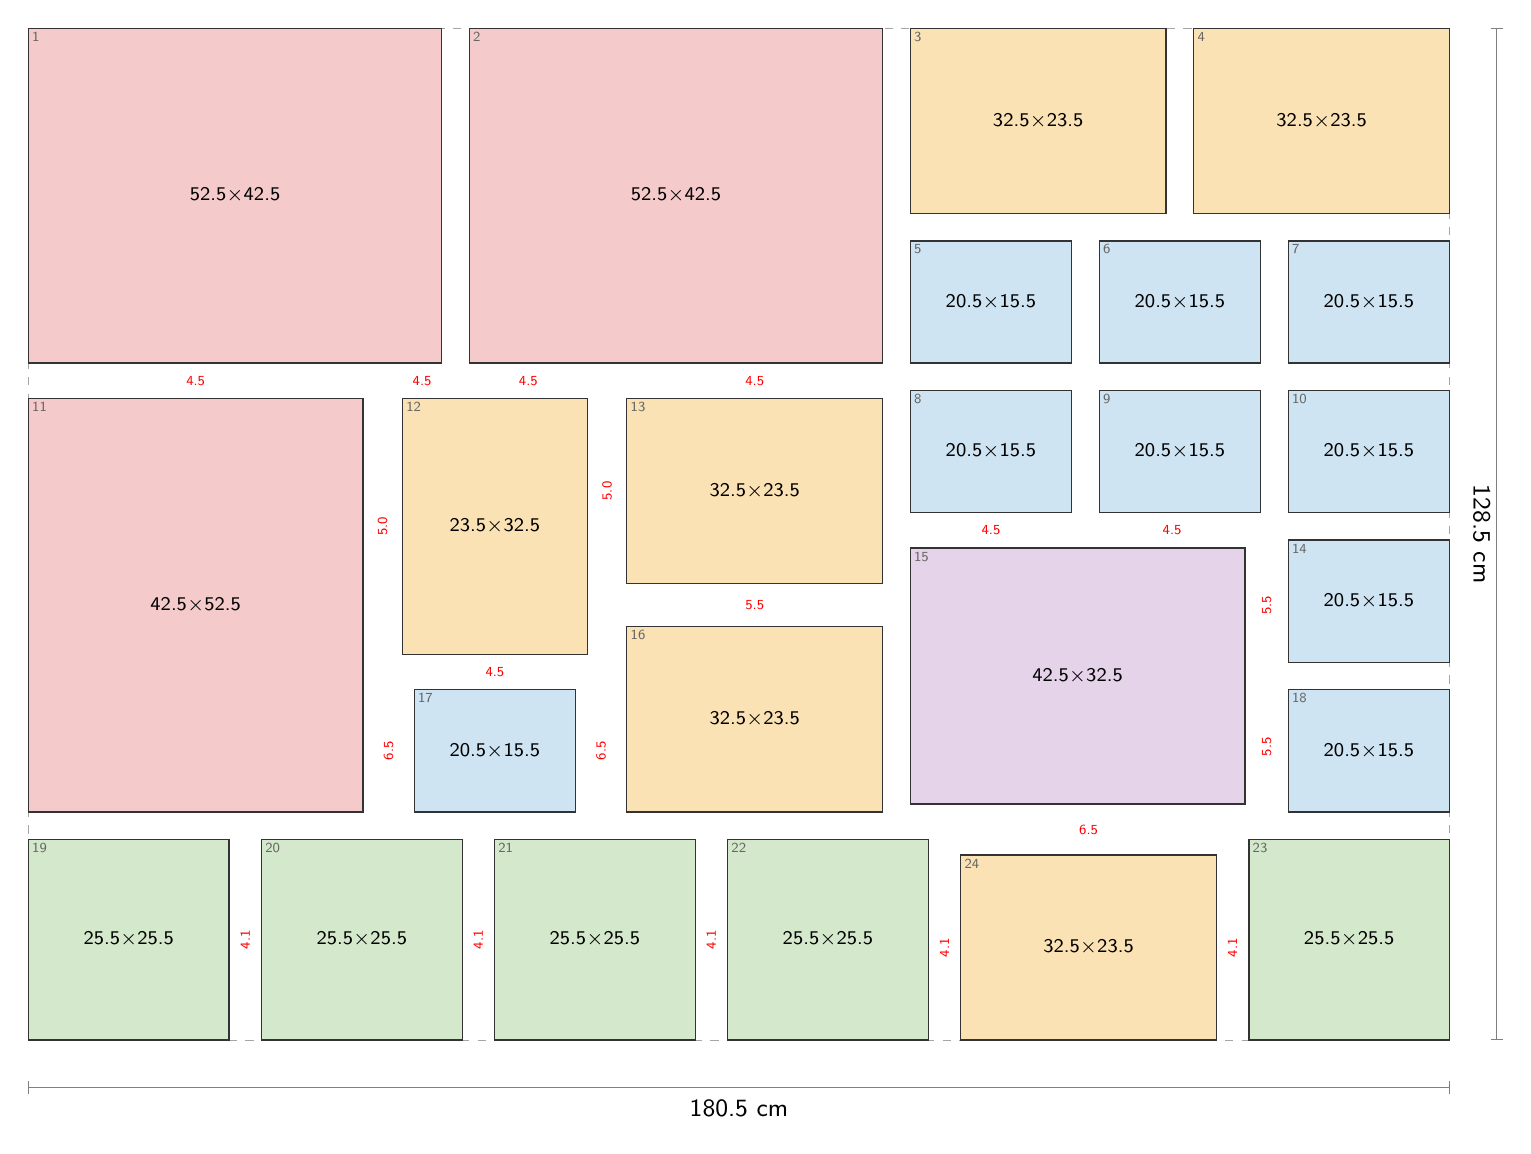
\begin{tikzpicture}[x=1mm, y=-1mm]
\draw[gray!70, dashed, line width=0.4pt] (0,0) rectangle (180.50,128.50);
\filldraw[fill=ft4, draw=black!80, line width=0.5pt] (0.00,0.00) rectangle (52.50,42.50);
\node[align=center, inner sep=0pt] at (26.25,21.25) {\scriptsize 52.5$\times$42.5};
\node[anchor=north west, inner sep=1.2pt, font=\tiny, text=black!60] at (0.00,0.00) {1};
\filldraw[fill=ft4, draw=black!80, line width=0.5pt] (56.00,0.00) rectangle (108.50,42.50);
\node[align=center, inner sep=0pt] at (82.25,21.25) {\scriptsize 52.5$\times$42.5};
\node[anchor=north west, inner sep=1.2pt, font=\tiny, text=black!60] at (56.00,0.00) {2};
\filldraw[fill=ft1, draw=black!80, line width=0.5pt] (112.00,0.00) rectangle (144.50,23.50);
\node[align=center, inner sep=0pt] at (128.25,11.75) {\scriptsize 32.5$\times$23.5};
\node[anchor=north west, inner sep=1.2pt, font=\tiny, text=black!60] at (112.00,0.00) {3};
\filldraw[fill=ft1, draw=black!80, line width=0.5pt] (148.00,0.00) rectangle (180.50,23.50);
\node[align=center, inner sep=0pt] at (164.25,11.75) {\scriptsize 32.5$\times$23.5};
\node[anchor=north west, inner sep=1.2pt, font=\tiny, text=black!60] at (148.00,0.00) {4};
\filldraw[fill=ft0, draw=black!80, line width=0.5pt] (112.00,27.00) rectangle (132.50,42.50);
\node[align=center, inner sep=0pt] at (122.25,34.75) {\scriptsize 20.5$\times$15.5};
\node[anchor=north west, inner sep=1.2pt, font=\tiny, text=black!60] at (112.00,27.00) {5};
\filldraw[fill=ft0, draw=black!80, line width=0.5pt] (136.00,27.00) rectangle (156.50,42.50);
\node[align=center, inner sep=0pt] at (146.25,34.75) {\scriptsize 20.5$\times$15.5};
\node[anchor=north west, inner sep=1.2pt, font=\tiny, text=black!60] at (136.00,27.00) {6};
\filldraw[fill=ft0, draw=black!80, line width=0.5pt] (160.00,27.00) rectangle (180.50,42.50);
\node[align=center, inner sep=0pt] at (170.25,34.75) {\scriptsize 20.5$\times$15.5};
\node[anchor=north west, inner sep=1.2pt, font=\tiny, text=black!60] at (160.00,27.00) {7};
\filldraw[fill=ft0, draw=black!80, line width=0.5pt] (112.00,46.00) rectangle (132.50,61.50);
\node[align=center, inner sep=0pt] at (122.25,53.75) {\scriptsize 20.5$\times$15.5};
\node[anchor=north west, inner sep=1.2pt, font=\tiny, text=black!60] at (112.00,46.00) {8};
\filldraw[fill=ft0, draw=black!80, line width=0.5pt] (136.00,46.00) rectangle (156.50,61.50);
\node[align=center, inner sep=0pt] at (146.25,53.75) {\scriptsize 20.5$\times$15.5};
\node[anchor=north west, inner sep=1.2pt, font=\tiny, text=black!60] at (136.00,46.00) {9};
\filldraw[fill=ft0, draw=black!80, line width=0.5pt] (160.00,46.00) rectangle (180.50,61.50);
\node[align=center, inner sep=0pt] at (170.25,53.75) {\scriptsize 20.5$\times$15.5};
\node[anchor=north west, inner sep=1.2pt, font=\tiny, text=black!60] at (160.00,46.00) {10};
\filldraw[fill=ft4, draw=black!80, line width=0.5pt] (0.00,47.00) rectangle (42.50,99.50);
\node[align=center, inner sep=0pt] at (21.25,73.25) {\scriptsize 42.5$\times$52.5};
\node[anchor=north west, inner sep=1.2pt, font=\tiny, text=black!60] at (0.00,47.00) {11};
\filldraw[fill=ft1, draw=black!80, line width=0.5pt] (47.50,47.00) rectangle (71.00,79.50);
\node[align=center, inner sep=0pt] at (59.25,63.25) {\scriptsize 23.5$\times$32.5};
\node[anchor=north west, inner sep=1.2pt, font=\tiny, text=black!60] at (47.50,47.00) {12};
\filldraw[fill=ft1, draw=black!80, line width=0.5pt] (76.00,47.00) rectangle (108.50,70.50);
\node[align=center, inner sep=0pt] at (92.25,58.75) {\scriptsize 32.5$\times$23.5};
\node[anchor=north west, inner sep=1.2pt, font=\tiny, text=black!60] at (76.00,47.00) {13};
\filldraw[fill=ft0, draw=black!80, line width=0.5pt] (160.00,65.00) rectangle (180.50,80.50);
\node[align=center, inner sep=0pt] at (170.25,72.75) {\scriptsize 20.5$\times$15.5};
\node[anchor=north west, inner sep=1.2pt, font=\tiny, text=black!60] at (160.00,65.00) {14};
\filldraw[fill=ft3, draw=black!80, line width=0.5pt] (112.00,66.00) rectangle (154.50,98.50);
\node[align=center, inner sep=0pt] at (133.25,82.25) {\scriptsize 42.5$\times$32.5};
\node[anchor=north west, inner sep=1.2pt, font=\tiny, text=black!60] at (112.00,66.00) {15};
\filldraw[fill=ft1, draw=black!80, line width=0.5pt] (76.00,76.00) rectangle (108.50,99.50);
\node[align=center, inner sep=0pt] at (92.25,87.75) {\scriptsize 32.5$\times$23.5};
\node[anchor=north west, inner sep=1.2pt, font=\tiny, text=black!60] at (76.00,76.00) {16};
\filldraw[fill=ft0, draw=black!80, line width=0.5pt] (49.00,84.00) rectangle (69.50,99.50);
\node[align=center, inner sep=0pt] at (59.25,91.75) {\scriptsize 20.5$\times$15.5};
\node[anchor=north west, inner sep=1.2pt, font=\tiny, text=black!60] at (49.00,84.00) {17};
\filldraw[fill=ft0, draw=black!80, line width=0.5pt] (160.00,84.00) rectangle (180.50,99.50);
\node[align=center, inner sep=0pt] at (170.25,91.75) {\scriptsize 20.5$\times$15.5};
\node[anchor=north west, inner sep=1.2pt, font=\tiny, text=black!60] at (160.00,84.00) {18};
\filldraw[fill=ft2, draw=black!80, line width=0.5pt] (0.00,103.00) rectangle (25.50,128.50);
\node[align=center, inner sep=0pt] at (12.75,115.75) {\scriptsize 25.5$\times$25.5};
\node[anchor=north west, inner sep=1.2pt, font=\tiny, text=black!60] at (0.00,103.00) {19};
\filldraw[fill=ft2, draw=black!80, line width=0.5pt] (29.60,103.00) rectangle (55.10,128.50);
\node[align=center, inner sep=0pt] at (42.35,115.75) {\scriptsize 25.5$\times$25.5};
\node[anchor=north west, inner sep=1.2pt, font=\tiny, text=black!60] at (29.60,103.00) {20};
\filldraw[fill=ft2, draw=black!80, line width=0.5pt] (59.20,103.00) rectangle (84.70,128.50);
\node[align=center, inner sep=0pt] at (71.95,115.75) {\scriptsize 25.5$\times$25.5};
\node[anchor=north west, inner sep=1.2pt, font=\tiny, text=black!60] at (59.20,103.00) {21};
\filldraw[fill=ft2, draw=black!80, line width=0.5pt] (88.80,103.00) rectangle (114.30,128.50);
\node[align=center, inner sep=0pt] at (101.55,115.75) {\scriptsize 25.5$\times$25.5};
\node[anchor=north west, inner sep=1.2pt, font=\tiny, text=black!60] at (88.80,103.00) {22};
\filldraw[fill=ft2, draw=black!80, line width=0.5pt] (155.00,103.00) rectangle (180.50,128.50);
\node[align=center, inner sep=0pt] at (167.75,115.75) {\scriptsize 25.5$\times$25.5};
\node[anchor=north west, inner sep=1.2pt, font=\tiny, text=black!60] at (155.00,103.00) {23};
\filldraw[fill=ft1, draw=black!80, line width=0.5pt] (118.40,105.00) rectangle (150.90,128.50);
\node[align=center, inner sep=0pt] at (134.65,116.75) {\scriptsize 32.5$\times$23.5};
\node[anchor=north west, inner sep=1.2pt, font=\tiny, text=black!60] at (118.40,105.00) {24};
\node[font=\tiny, text=red, fill=white, inner sep=0.3pt] at (21.25,44.75) {4.5};
\node[font=\tiny, text=red, fill=white, inner sep=0.3pt] at (50.00,44.75) {4.5};
\node[font=\tiny, text=red, fill=white, inner sep=0.3pt] at (63.50,44.75) {4.5};
\node[font=\tiny, text=red, fill=white, inner sep=0.3pt] at (92.25,44.75) {4.5};
\node[font=\tiny, text=red, fill=white, inner sep=0.3pt] at (122.25,63.75) {4.5};
\node[font=\tiny, text=red, fill=white, inner sep=0.3pt] at (145.25,63.75) {4.5};
\node[font=\tiny, text=red, fill=white, inner sep=0.3pt, rotate=90] at (45.00,63.25) {5.0};
\node[font=\tiny, text=red, fill=white, inner sep=0.3pt, rotate=90] at (45.75,91.75) {6.5};
\node[font=\tiny, text=red, fill=white, inner sep=0.3pt, rotate=90] at (73.50,58.75) {5.0};
\node[font=\tiny, text=red, fill=white, inner sep=0.3pt] at (59.25,81.75) {4.5};
\node[font=\tiny, text=red, fill=white, inner sep=0.3pt] at (92.25,73.25) {5.5};
\node[font=\tiny, text=red, fill=white, inner sep=0.3pt, rotate=90] at (157.25,73.25) {5.5};
\node[font=\tiny, text=red, fill=white, inner sep=0.3pt, rotate=90] at (157.25,91.25) {5.5};
\node[font=\tiny, text=red, fill=white, inner sep=0.3pt] at (134.65,101.75) {6.5};
\node[font=\tiny, text=red, fill=white, inner sep=0.3pt, rotate=90] at (72.75,91.75) {6.5};
\node[font=\tiny, text=red, fill=white, inner sep=0.3pt, rotate=90] at (27.55,115.75) {4.1};
\node[font=\tiny, text=red, fill=white, inner sep=0.3pt, rotate=90] at (57.15,115.75) {4.1};
\node[font=\tiny, text=red, fill=white, inner sep=0.3pt, rotate=90] at (86.75,115.75) {4.1};
\node[font=\tiny, text=red, fill=white, inner sep=0.3pt, rotate=90] at (116.35,116.75) {4.1};
\node[font=\tiny, text=red, fill=white, inner sep=0.3pt, rotate=90] at (152.95,116.75) {4.1};
\draw[Bar-Bar, gray] (0,134.50) -- (180.50,134.50) node[midway, below=1pt, font=\small, text=black] {180.5 cm};
\draw[Bar-Bar, gray] (186.50,0) -- (186.50,128.50) node[midway, right=1pt, font=\small, text=black, rotate=-90, anchor=north] {128.5 cm};
\end{tikzpicture}\\[4pt]
{\scriptsize Scale 1:10 (1 mm = 1 cm). Red numbers mark gaps that deviate from the nominal gap by more than 0.25 cm. Small grey numbers index the coordinate table.}
\end{minipage}\hfill
\begin{minipage}[t]{0.25\textwidth}\vspace{0pt}
\small
\begin{tabular}{@{}l l@{}}
\toprule
Outer size & 180.5 $\times$ 128.5 cm \\
Nominal gap & 3.5 cm \\
Actual gaps & 3.5 -- 6.5 cm \\
Max.\ deviation & 3.0 cm \\
Mean deviation & 0.61 cm \\
Border notches & none \\
Corners filled & 4 / 4 \\
Frames used & 24 of 28 \\
\bottomrule
\end{tabular}

\vspace{8pt}
\scriptsize
\begin{tabular}{@{}c l l r r@{}}
\toprule
 & outer w $\times$ h (cm) & & used & have \\
\midrule
\tikz[baseline=-0.6ex]\fill[ft0,draw=black!60] (0,0) rectangle (1.2ex,1.2ex); & 20.5$\times$15.5 & L & 9 & 9 \\
\tikz[baseline=-0.6ex]\fill[ft0,draw=black!60] (0,0) rectangle (1.2ex,1.2ex); & 15.5$\times$20.5 & P & 0 & 2 \\
\tikz[baseline=-0.6ex]\fill[ft3,draw=black!60] (0,0) rectangle (1.2ex,1.2ex); & 32.5$\times$42.5 & P & 0 & 2 \\
\tikz[baseline=-0.6ex]\fill[ft3,draw=black!60] (0,0) rectangle (1.2ex,1.2ex); & 42.5$\times$32.5 & L & 1 & 1 \\
\tikz[baseline=-0.6ex]\fill[ft1,draw=black!60] (0,0) rectangle (1.2ex,1.2ex); & 32.5$\times$23.5 & L & 5 & 5 \\
\tikz[baseline=-0.6ex]\fill[ft1,draw=black!60] (0,0) rectangle (1.2ex,1.2ex); & 23.5$\times$32.5 & P & 1 & 1 \\
\tikz[baseline=-0.6ex]\fill[ft2,draw=black!60] (0,0) rectangle (1.2ex,1.2ex); & 25.5$\times$25.5 &  & 5 & 5 \\
\tikz[baseline=-0.6ex]\fill[ft4,draw=black!60] (0,0) rectangle (1.2ex,1.2ex); & 42.5$\times$52.5 & P & 1 & 1 \\
\tikz[baseline=-0.6ex]\fill[ft4,draw=black!60] (0,0) rectangle (1.2ex,1.2ex); & 52.5$\times$42.5 & L & 2 & 2 \\
\bottomrule
\end{tabular}

\vspace{8pt}
{\bfseries Positions} (top-left corner, cm)\\[2pt]
\tiny
\begin{tabular}{@{}r l r r@{}}
\toprule
\# & frame w $\times$ h & x & y \\
\midrule
1 & 52.5 $\times$ 42.5 & 0.0 & 0.0 \\
2 & 52.5 $\times$ 42.5 & 56.0 & 0.0 \\
3 & 32.5 $\times$ 23.5 & 112.0 & 0.0 \\
4 & 32.5 $\times$ 23.5 & 148.0 & 0.0 \\
5 & 20.5 $\times$ 15.5 & 112.0 & 27.0 \\
6 & 20.5 $\times$ 15.5 & 136.0 & 27.0 \\
7 & 20.5 $\times$ 15.5 & 160.0 & 27.0 \\
8 & 20.5 $\times$ 15.5 & 112.0 & 46.0 \\
9 & 20.5 $\times$ 15.5 & 136.0 & 46.0 \\
10 & 20.5 $\times$ 15.5 & 160.0 & 46.0 \\
11 & 42.5 $\times$ 52.5 & 0.0 & 47.0 \\
12 & 23.5 $\times$ 32.5 & 47.5 & 47.0 \\
13 & 32.5 $\times$ 23.5 & 76.0 & 47.0 \\
14 & 20.5 $\times$ 15.5 & 160.0 & 65.0 \\
15 & 42.5 $\times$ 32.5 & 112.0 & 66.0 \\
16 & 32.5 $\times$ 23.5 & 76.0 & 76.0 \\
17 & 20.5 $\times$ 15.5 & 49.0 & 84.0 \\
18 & 20.5 $\times$ 15.5 & 160.0 & 84.0 \\
19 & 25.5 $\times$ 25.5 & 0.0 & 103.0 \\
20 & 25.5 $\times$ 25.5 & 29.6 & 103.0 \\
21 & 25.5 $\times$ 25.5 & 59.2 & 103.0 \\
22 & 25.5 $\times$ 25.5 & 88.8 & 103.0 \\
23 & 25.5 $\times$ 25.5 & 155.0 & 103.0 \\
24 & 32.5 $\times$ 23.5 & 118.4 & 105.0 \\
\bottomrule
\end{tabular}
\end{minipage}
\clearpage

\begin{minipage}[t]{0.74\textwidth}\vspace{0pt}
{\LARGE\bfseries Layout 8}\hspace{1.5em}{\large 169.5 $\times$ 113.5 cm \quad gap 1.5 cm \quad 23 frames}\\[8pt]
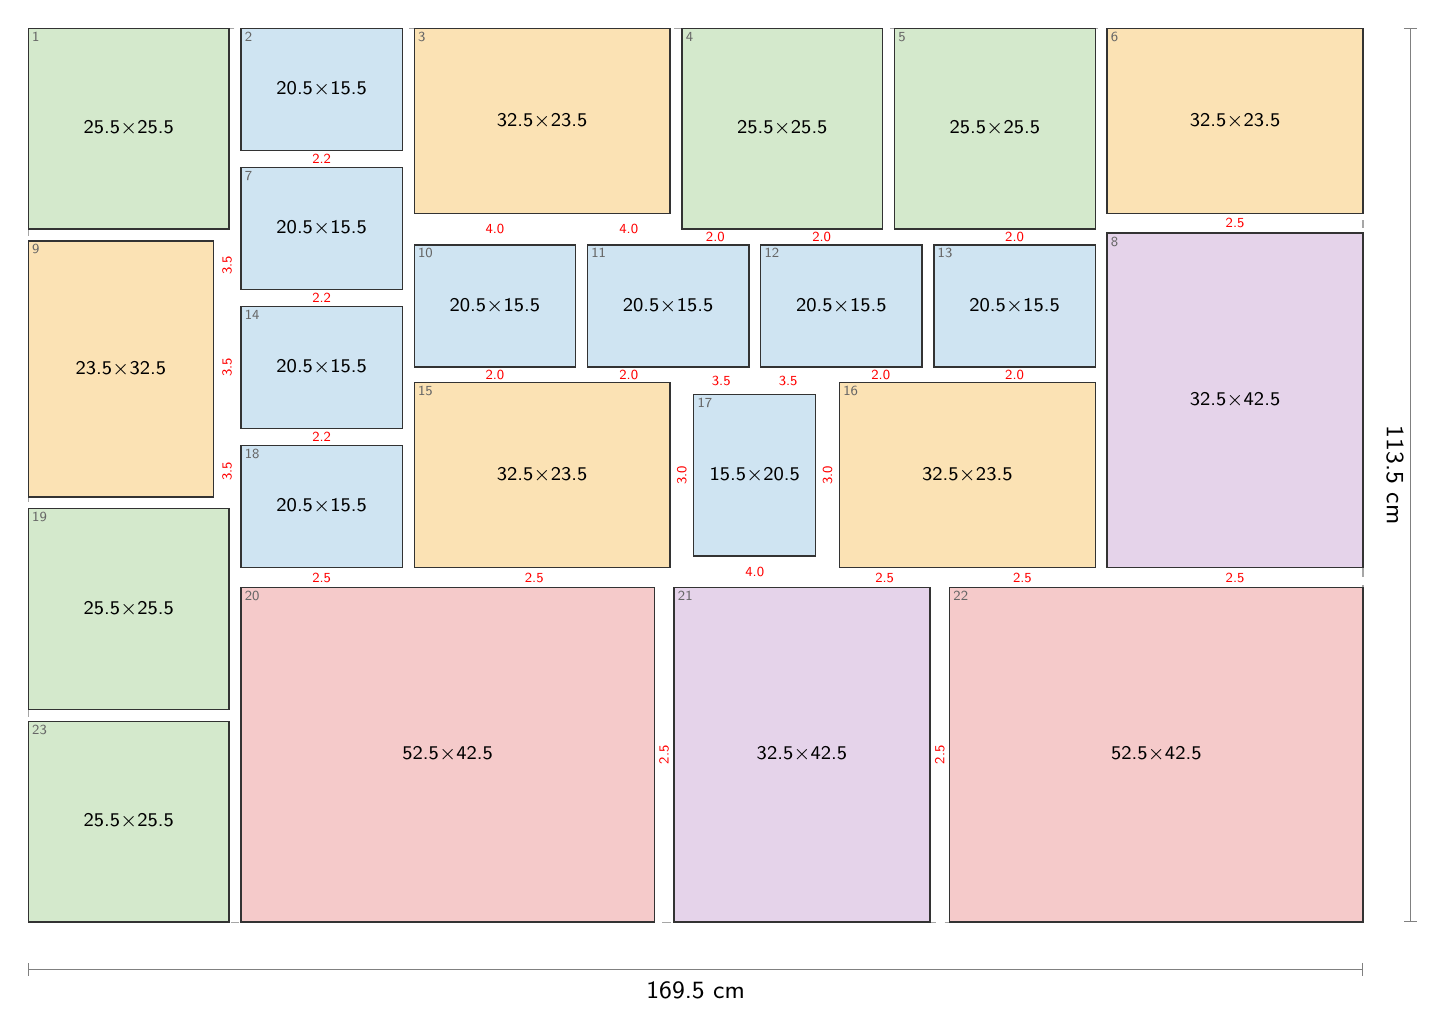
\begin{tikzpicture}[x=1mm, y=-1mm]
\draw[gray!70, dashed, line width=0.4pt] (0,0) rectangle (169.50,113.50);
\filldraw[fill=ft2, draw=black!80, line width=0.5pt] (0.00,0.00) rectangle (25.50,25.50);
\node[align=center, inner sep=0pt] at (12.75,12.75) {\scriptsize 25.5$\times$25.5};
\node[anchor=north west, inner sep=1.2pt, font=\tiny, text=black!60] at (0.00,0.00) {1};
\filldraw[fill=ft0, draw=black!80, line width=0.5pt] (27.00,0.00) rectangle (47.50,15.50);
\node[align=center, inner sep=0pt] at (37.25,7.75) {\scriptsize 20.5$\times$15.5};
\node[anchor=north west, inner sep=1.2pt, font=\tiny, text=black!60] at (27.00,0.00) {2};
\filldraw[fill=ft1, draw=black!80, line width=0.5pt] (49.00,0.00) rectangle (81.50,23.50);
\node[align=center, inner sep=0pt] at (65.25,11.75) {\scriptsize 32.5$\times$23.5};
\node[anchor=north west, inner sep=1.2pt, font=\tiny, text=black!60] at (49.00,0.00) {3};
\filldraw[fill=ft2, draw=black!80, line width=0.5pt] (83.00,0.00) rectangle (108.50,25.50);
\node[align=center, inner sep=0pt] at (95.75,12.75) {\scriptsize 25.5$\times$25.5};
\node[anchor=north west, inner sep=1.2pt, font=\tiny, text=black!60] at (83.00,0.00) {4};
\filldraw[fill=ft2, draw=black!80, line width=0.5pt] (110.00,0.00) rectangle (135.50,25.50);
\node[align=center, inner sep=0pt] at (122.75,12.75) {\scriptsize 25.5$\times$25.5};
\node[anchor=north west, inner sep=1.2pt, font=\tiny, text=black!60] at (110.00,0.00) {5};
\filldraw[fill=ft1, draw=black!80, line width=0.5pt] (137.00,0.00) rectangle (169.50,23.50);
\node[align=center, inner sep=0pt] at (153.25,11.75) {\scriptsize 32.5$\times$23.5};
\node[anchor=north west, inner sep=1.2pt, font=\tiny, text=black!60] at (137.00,0.00) {6};
\filldraw[fill=ft0, draw=black!80, line width=0.5pt] (27.00,17.67) rectangle (47.50,33.17);
\node[align=center, inner sep=0pt] at (37.25,25.42) {\scriptsize 20.5$\times$15.5};
\node[anchor=north west, inner sep=1.2pt, font=\tiny, text=black!60] at (27.00,17.67) {7};
\filldraw[fill=ft3, draw=black!80, line width=0.5pt] (137.00,26.00) rectangle (169.50,68.50);
\node[align=center, inner sep=0pt] at (153.25,47.25) {\scriptsize 32.5$\times$42.5};
\node[anchor=north west, inner sep=1.2pt, font=\tiny, text=black!60] at (137.00,26.00) {8};
\filldraw[fill=ft1, draw=black!80, line width=0.5pt] (0.00,27.00) rectangle (23.50,59.50);
\node[align=center, inner sep=0pt] at (11.75,43.25) {\scriptsize 23.5$\times$32.5};
\node[anchor=north west, inner sep=1.2pt, font=\tiny, text=black!60] at (0.00,27.00) {9};
\filldraw[fill=ft0, draw=black!80, line width=0.5pt] (49.00,27.50) rectangle (69.50,43.00);
\node[align=center, inner sep=0pt] at (59.25,35.25) {\scriptsize 20.5$\times$15.5};
\node[anchor=north west, inner sep=1.2pt, font=\tiny, text=black!60] at (49.00,27.50) {10};
\filldraw[fill=ft0, draw=black!80, line width=0.5pt] (71.00,27.50) rectangle (91.50,43.00);
\node[align=center, inner sep=0pt] at (81.25,35.25) {\scriptsize 20.5$\times$15.5};
\node[anchor=north west, inner sep=1.2pt, font=\tiny, text=black!60] at (71.00,27.50) {11};
\filldraw[fill=ft0, draw=black!80, line width=0.5pt] (93.00,27.50) rectangle (113.50,43.00);
\node[align=center, inner sep=0pt] at (103.25,35.25) {\scriptsize 20.5$\times$15.5};
\node[anchor=north west, inner sep=1.2pt, font=\tiny, text=black!60] at (93.00,27.50) {12};
\filldraw[fill=ft0, draw=black!80, line width=0.5pt] (115.00,27.50) rectangle (135.50,43.00);
\node[align=center, inner sep=0pt] at (125.25,35.25) {\scriptsize 20.5$\times$15.5};
\node[anchor=north west, inner sep=1.2pt, font=\tiny, text=black!60] at (115.00,27.50) {13};
\filldraw[fill=ft0, draw=black!80, line width=0.5pt] (27.00,35.33) rectangle (47.50,50.83);
\node[align=center, inner sep=0pt] at (37.25,43.08) {\scriptsize 20.5$\times$15.5};
\node[anchor=north west, inner sep=1.2pt, font=\tiny, text=black!60] at (27.00,35.33) {14};
\filldraw[fill=ft1, draw=black!80, line width=0.5pt] (49.00,45.00) rectangle (81.50,68.50);
\node[align=center, inner sep=0pt] at (65.25,56.75) {\scriptsize 32.5$\times$23.5};
\node[anchor=north west, inner sep=1.2pt, font=\tiny, text=black!60] at (49.00,45.00) {15};
\filldraw[fill=ft1, draw=black!80, line width=0.5pt] (103.00,45.00) rectangle (135.50,68.50);
\node[align=center, inner sep=0pt] at (119.25,56.75) {\scriptsize 32.5$\times$23.5};
\node[anchor=north west, inner sep=1.2pt, font=\tiny, text=black!60] at (103.00,45.00) {16};
\filldraw[fill=ft0, draw=black!80, line width=0.5pt] (84.50,46.50) rectangle (100.00,67.00);
\node[align=center, inner sep=0pt] at (92.25,56.75) {\scriptsize 15.5$\times$20.5};
\node[anchor=north west, inner sep=1.2pt, font=\tiny, text=black!60] at (84.50,46.50) {17};
\filldraw[fill=ft0, draw=black!80, line width=0.5pt] (27.00,53.00) rectangle (47.50,68.50);
\node[align=center, inner sep=0pt] at (37.25,60.75) {\scriptsize 20.5$\times$15.5};
\node[anchor=north west, inner sep=1.2pt, font=\tiny, text=black!60] at (27.00,53.00) {18};
\filldraw[fill=ft2, draw=black!80, line width=0.5pt] (0.00,61.00) rectangle (25.50,86.50);
\node[align=center, inner sep=0pt] at (12.75,73.75) {\scriptsize 25.5$\times$25.5};
\node[anchor=north west, inner sep=1.2pt, font=\tiny, text=black!60] at (0.00,61.00) {19};
\filldraw[fill=ft4, draw=black!80, line width=0.5pt] (27.00,71.00) rectangle (79.50,113.50);
\node[align=center, inner sep=0pt] at (53.25,92.25) {\scriptsize 52.5$\times$42.5};
\node[anchor=north west, inner sep=1.2pt, font=\tiny, text=black!60] at (27.00,71.00) {20};
\filldraw[fill=ft3, draw=black!80, line width=0.5pt] (82.00,71.00) rectangle (114.50,113.50);
\node[align=center, inner sep=0pt] at (98.25,92.25) {\scriptsize 32.5$\times$42.5};
\node[anchor=north west, inner sep=1.2pt, font=\tiny, text=black!60] at (82.00,71.00) {21};
\filldraw[fill=ft4, draw=black!80, line width=0.5pt] (117.00,71.00) rectangle (169.50,113.50);
\node[align=center, inner sep=0pt] at (143.25,92.25) {\scriptsize 52.5$\times$42.5};
\node[anchor=north west, inner sep=1.2pt, font=\tiny, text=black!60] at (117.00,71.00) {22};
\filldraw[fill=ft2, draw=black!80, line width=0.5pt] (0.00,88.00) rectangle (25.50,113.50);
\node[align=center, inner sep=0pt] at (12.75,100.75) {\scriptsize 25.5$\times$25.5};
\node[anchor=north west, inner sep=1.2pt, font=\tiny, text=black!60] at (0.00,88.00) {23};
\node[font=\tiny, text=red, fill=white, inner sep=0.3pt] at (37.25,16.58) {2.2};
\node[font=\tiny, text=red, fill=white, inner sep=0.3pt] at (59.25,25.50) {4.0};
\node[font=\tiny, text=red, fill=white, inner sep=0.3pt] at (76.25,25.50) {4.0};
\node[font=\tiny, text=red, fill=white, inner sep=0.3pt] at (87.25,26.50) {2.0};
\node[font=\tiny, text=red, fill=white, inner sep=0.3pt] at (100.75,26.50) {2.0};
\node[font=\tiny, text=red, fill=white, inner sep=0.3pt] at (125.25,26.50) {2.0};
\node[font=\tiny, text=red, fill=white, inner sep=0.3pt] at (153.25,24.75) {2.5};
\node[font=\tiny, text=red, fill=white, inner sep=0.3pt] at (37.25,34.25) {2.2};
\node[font=\tiny, text=red, fill=white, inner sep=0.3pt] at (153.25,69.75) {2.5};
\node[font=\tiny, text=red, fill=white, inner sep=0.3pt, rotate=90] at (25.25,30.08) {3.5};
\node[font=\tiny, text=red, fill=white, inner sep=0.3pt, rotate=90] at (25.25,43.08) {3.5};
\node[font=\tiny, text=red, fill=white, inner sep=0.3pt, rotate=90] at (25.25,56.25) {3.5};
\node[font=\tiny, text=red, fill=white, inner sep=0.3pt] at (59.25,44.00) {2.0};
\node[font=\tiny, text=red, fill=white, inner sep=0.3pt] at (76.25,44.00) {2.0};
\node[font=\tiny, text=red, fill=white, inner sep=0.3pt] at (88.00,44.75) {3.5};
\node[font=\tiny, text=red, fill=white, inner sep=0.3pt] at (108.25,44.00) {2.0};
\node[font=\tiny, text=red, fill=white, inner sep=0.3pt] at (96.50,44.75) {3.5};
\node[font=\tiny, text=red, fill=white, inner sep=0.3pt] at (125.25,44.00) {2.0};
\node[font=\tiny, text=red, fill=white, inner sep=0.3pt] at (37.25,51.92) {2.2};
\node[font=\tiny, text=red, fill=white, inner sep=0.3pt, rotate=90] at (83.00,56.75) {3.0};
\node[font=\tiny, text=red, fill=white, inner sep=0.3pt] at (64.25,69.75) {2.5};
\node[font=\tiny, text=red, fill=white, inner sep=0.3pt] at (108.75,69.75) {2.5};
\node[font=\tiny, text=red, fill=white, inner sep=0.3pt] at (126.25,69.75) {2.5};
\node[font=\tiny, text=red, fill=white, inner sep=0.3pt, rotate=90] at (101.50,56.75) {3.0};
\node[font=\tiny, text=red, fill=white, inner sep=0.3pt] at (92.25,69.00) {4.0};
\node[font=\tiny, text=red, fill=white, inner sep=0.3pt] at (37.25,69.75) {2.5};
\node[font=\tiny, text=red, fill=white, inner sep=0.3pt, rotate=90] at (80.75,92.25) {2.5};
\node[font=\tiny, text=red, fill=white, inner sep=0.3pt, rotate=90] at (115.75,92.25) {2.5};
\draw[Bar-Bar, gray] (0,119.50) -- (169.50,119.50) node[midway, below=1pt, font=\small, text=black] {169.5 cm};
\draw[Bar-Bar, gray] (175.50,0) -- (175.50,113.50) node[midway, right=1pt, font=\small, text=black, rotate=-90, anchor=north] {113.5 cm};
\end{tikzpicture}\\[4pt]
{\scriptsize Scale 1:10 (1 mm = 1 cm). Red numbers mark gaps that deviate from the nominal gap by more than 0.25 cm. Small grey numbers index the coordinate table.}
\end{minipage}\hfill
\begin{minipage}[t]{0.25\textwidth}\vspace{0pt}
\small
\begin{tabular}{@{}l l@{}}
\toprule
Outer size & 169.5 $\times$ 113.5 cm \\
Nominal gap & 1.5 cm \\
Actual gaps & 1.5 -- 4.0 cm \\
Max.\ deviation & 2.5 cm \\
Mean deviation & 0.68 cm \\
Border notches & none \\
Corners filled & 4 / 4 \\
Frames used & 23 of 28 \\
\bottomrule
\end{tabular}

\vspace{8pt}
\scriptsize
\begin{tabular}{@{}c l l r r@{}}
\toprule
 & outer w $\times$ h (cm) & & used & have \\
\midrule
\tikz[baseline=-0.6ex]\fill[ft0,draw=black!60] (0,0) rectangle (1.2ex,1.2ex); & 20.5$\times$15.5 & L & 8 & 9 \\
\tikz[baseline=-0.6ex]\fill[ft0,draw=black!60] (0,0) rectangle (1.2ex,1.2ex); & 15.5$\times$20.5 & P & 1 & 2 \\
\tikz[baseline=-0.6ex]\fill[ft3,draw=black!60] (0,0) rectangle (1.2ex,1.2ex); & 32.5$\times$42.5 & P & 2 & 2 \\
\tikz[baseline=-0.6ex]\fill[ft3,draw=black!60] (0,0) rectangle (1.2ex,1.2ex); & 42.5$\times$32.5 & L & 0 & 1 \\
\tikz[baseline=-0.6ex]\fill[ft1,draw=black!60] (0,0) rectangle (1.2ex,1.2ex); & 32.5$\times$23.5 & L & 4 & 5 \\
\tikz[baseline=-0.6ex]\fill[ft1,draw=black!60] (0,0) rectangle (1.2ex,1.2ex); & 23.5$\times$32.5 & P & 1 & 1 \\
\tikz[baseline=-0.6ex]\fill[ft2,draw=black!60] (0,0) rectangle (1.2ex,1.2ex); & 25.5$\times$25.5 &  & 5 & 5 \\
\tikz[baseline=-0.6ex]\fill[ft4,draw=black!60] (0,0) rectangle (1.2ex,1.2ex); & 42.5$\times$52.5 & P & 0 & 1 \\
\tikz[baseline=-0.6ex]\fill[ft4,draw=black!60] (0,0) rectangle (1.2ex,1.2ex); & 52.5$\times$42.5 & L & 2 & 2 \\
\bottomrule
\end{tabular}

\vspace{8pt}
{\bfseries Positions} (top-left corner, cm)\\[2pt]
\tiny
\begin{tabular}{@{}r l r r@{}}
\toprule
\# & frame w $\times$ h & x & y \\
\midrule
1 & 25.5 $\times$ 25.5 & 0.0 & 0.0 \\
2 & 20.5 $\times$ 15.5 & 27.0 & 0.0 \\
3 & 32.5 $\times$ 23.5 & 49.0 & 0.0 \\
4 & 25.5 $\times$ 25.5 & 83.0 & 0.0 \\
5 & 25.5 $\times$ 25.5 & 110.0 & 0.0 \\
6 & 32.5 $\times$ 23.5 & 137.0 & 0.0 \\
7 & 20.5 $\times$ 15.5 & 27.0 & 17.7 \\
8 & 32.5 $\times$ 42.5 & 137.0 & 26.0 \\
9 & 23.5 $\times$ 32.5 & 0.0 & 27.0 \\
10 & 20.5 $\times$ 15.5 & 49.0 & 27.5 \\
11 & 20.5 $\times$ 15.5 & 71.0 & 27.5 \\
12 & 20.5 $\times$ 15.5 & 93.0 & 27.5 \\
13 & 20.5 $\times$ 15.5 & 115.0 & 27.5 \\
14 & 20.5 $\times$ 15.5 & 27.0 & 35.3 \\
15 & 32.5 $\times$ 23.5 & 49.0 & 45.0 \\
16 & 32.5 $\times$ 23.5 & 103.0 & 45.0 \\
17 & 15.5 $\times$ 20.5 & 84.5 & 46.5 \\
18 & 20.5 $\times$ 15.5 & 27.0 & 53.0 \\
19 & 25.5 $\times$ 25.5 & 0.0 & 61.0 \\
20 & 52.5 $\times$ 42.5 & 27.0 & 71.0 \\
21 & 32.5 $\times$ 42.5 & 82.0 & 71.0 \\
22 & 52.5 $\times$ 42.5 & 117.0 & 71.0 \\
23 & 25.5 $\times$ 25.5 & 0.0 & 88.0 \\
\bottomrule
\end{tabular}
\end{minipage}
\clearpage

\begin{minipage}[t]{0.74\textwidth}\vspace{0pt}
{\LARGE\bfseries Layout 9}\hspace{1.5em}{\large 184.0 $\times$ 115.0 cm \quad gap 2 cm \quad 23 frames}\\[8pt]
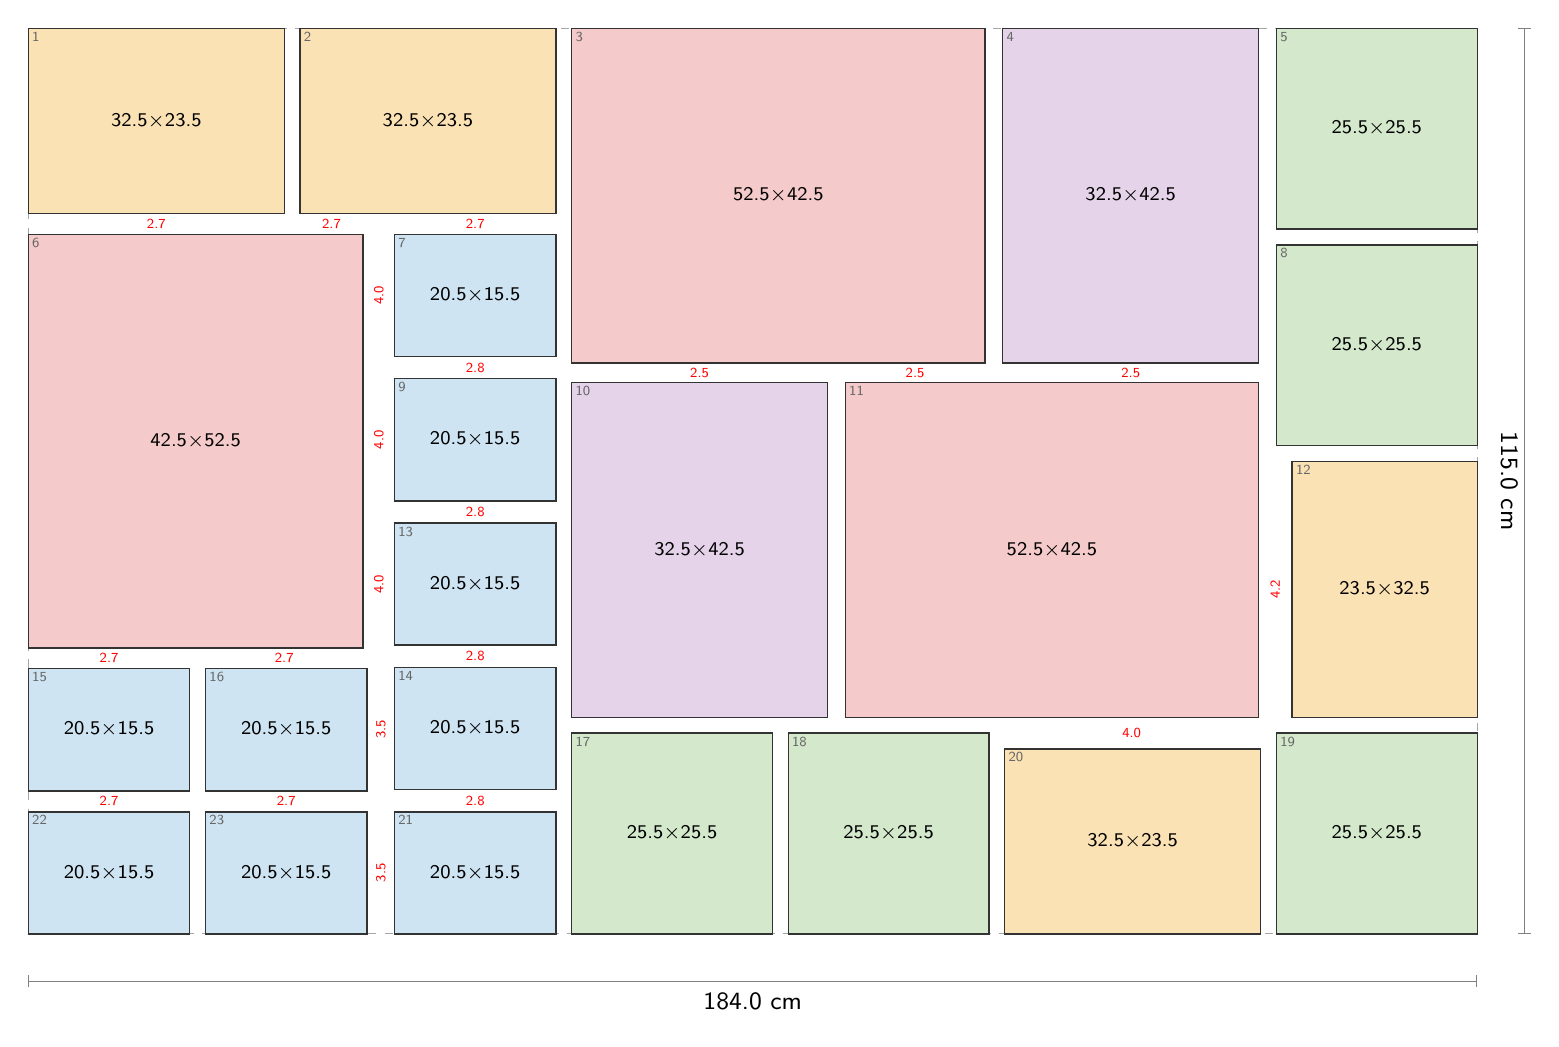
\begin{tikzpicture}[x=1mm, y=-1mm]
\draw[gray!70, dashed, line width=0.4pt] (0,0) rectangle (184.00,115.00);
\filldraw[fill=ft1, draw=black!80, line width=0.5pt] (0.00,0.00) rectangle (32.50,23.50);
\node[align=center, inner sep=0pt] at (16.25,11.75) {\scriptsize 32.5$\times$23.5};
\node[anchor=north west, inner sep=1.2pt, font=\tiny, text=black!60] at (0.00,0.00) {1};
\filldraw[fill=ft1, draw=black!80, line width=0.5pt] (34.50,0.00) rectangle (67.00,23.50);
\node[align=center, inner sep=0pt] at (50.75,11.75) {\scriptsize 32.5$\times$23.5};
\node[anchor=north west, inner sep=1.2pt, font=\tiny, text=black!60] at (34.50,0.00) {2};
\filldraw[fill=ft4, draw=black!80, line width=0.5pt] (69.00,0.00) rectangle (121.50,42.50);
\node[align=center, inner sep=0pt] at (95.25,21.25) {\scriptsize 52.5$\times$42.5};
\node[anchor=north west, inner sep=1.2pt, font=\tiny, text=black!60] at (69.00,0.00) {3};
\filldraw[fill=ft3, draw=black!80, line width=0.5pt] (123.75,0.00) rectangle (156.25,42.50);
\node[align=center, inner sep=0pt] at (140.00,21.25) {\scriptsize 32.5$\times$42.5};
\node[anchor=north west, inner sep=1.2pt, font=\tiny, text=black!60] at (123.75,0.00) {4};
\filldraw[fill=ft2, draw=black!80, line width=0.5pt] (158.50,0.00) rectangle (184.00,25.50);
\node[align=center, inner sep=0pt] at (171.25,12.75) {\scriptsize 25.5$\times$25.5};
\node[anchor=north west, inner sep=1.2pt, font=\tiny, text=black!60] at (158.50,0.00) {5};
\filldraw[fill=ft4, draw=black!80, line width=0.5pt] (0.00,26.17) rectangle (42.50,78.67);
\node[align=center, inner sep=0pt] at (21.25,52.42) {\scriptsize 42.5$\times$52.5};
\node[anchor=north west, inner sep=1.2pt, font=\tiny, text=black!60] at (0.00,26.17) {6};
\filldraw[fill=ft0, draw=black!80, line width=0.5pt] (46.50,26.17) rectangle (67.00,41.67);
\node[align=center, inner sep=0pt] at (56.75,33.92) {\scriptsize 20.5$\times$15.5};
\node[anchor=north west, inner sep=1.2pt, font=\tiny, text=black!60] at (46.50,26.17) {7};
\filldraw[fill=ft2, draw=black!80, line width=0.5pt] (158.50,27.50) rectangle (184.00,53.00);
\node[align=center, inner sep=0pt] at (171.25,40.25) {\scriptsize 25.5$\times$25.5};
\node[anchor=north west, inner sep=1.2pt, font=\tiny, text=black!60] at (158.50,27.50) {8};
\filldraw[fill=ft0, draw=black!80, line width=0.5pt] (46.50,44.50) rectangle (67.00,60.00);
\node[align=center, inner sep=0pt] at (56.75,52.25) {\scriptsize 20.5$\times$15.5};
\node[anchor=north west, inner sep=1.2pt, font=\tiny, text=black!60] at (46.50,44.50) {9};
\filldraw[fill=ft3, draw=black!80, line width=0.5pt] (69.00,45.00) rectangle (101.50,87.50);
\node[align=center, inner sep=0pt] at (85.25,66.25) {\scriptsize 32.5$\times$42.5};
\node[anchor=north west, inner sep=1.2pt, font=\tiny, text=black!60] at (69.00,45.00) {10};
\filldraw[fill=ft4, draw=black!80, line width=0.5pt] (103.75,45.00) rectangle (156.25,87.50);
\node[align=center, inner sep=0pt] at (130.00,66.25) {\scriptsize 52.5$\times$42.5};
\node[anchor=north west, inner sep=1.2pt, font=\tiny, text=black!60] at (103.75,45.00) {11};
\filldraw[fill=ft1, draw=black!80, line width=0.5pt] (160.50,55.00) rectangle (184.00,87.50);
\node[align=center, inner sep=0pt] at (172.25,71.25) {\scriptsize 23.5$\times$32.5};
\node[anchor=north west, inner sep=1.2pt, font=\tiny, text=black!60] at (160.50,55.00) {12};
\filldraw[fill=ft0, draw=black!80, line width=0.5pt] (46.50,62.83) rectangle (67.00,78.33);
\node[align=center, inner sep=0pt] at (56.75,70.58) {\scriptsize 20.5$\times$15.5};
\node[anchor=north west, inner sep=1.2pt, font=\tiny, text=black!60] at (46.50,62.83) {13};
\filldraw[fill=ft0, draw=black!80, line width=0.5pt] (46.50,81.17) rectangle (67.00,96.67);
\node[align=center, inner sep=0pt] at (56.75,88.92) {\scriptsize 20.5$\times$15.5};
\node[anchor=north west, inner sep=1.2pt, font=\tiny, text=black!60] at (46.50,81.17) {14};
\filldraw[fill=ft0, draw=black!80, line width=0.5pt] (0.00,81.33) rectangle (20.50,96.83);
\node[align=center, inner sep=0pt] at (10.25,89.08) {\scriptsize 20.5$\times$15.5};
\node[anchor=north west, inner sep=1.2pt, font=\tiny, text=black!60] at (0.00,81.33) {15};
\filldraw[fill=ft0, draw=black!80, line width=0.5pt] (22.50,81.33) rectangle (43.00,96.83);
\node[align=center, inner sep=0pt] at (32.75,89.08) {\scriptsize 20.5$\times$15.5};
\node[anchor=north west, inner sep=1.2pt, font=\tiny, text=black!60] at (22.50,81.33) {16};
\filldraw[fill=ft2, draw=black!80, line width=0.5pt] (69.00,89.50) rectangle (94.50,115.00);
\node[align=center, inner sep=0pt] at (81.75,102.25) {\scriptsize 25.5$\times$25.5};
\node[anchor=north west, inner sep=1.2pt, font=\tiny, text=black!60] at (69.00,89.50) {17};
\filldraw[fill=ft2, draw=black!80, line width=0.5pt] (96.50,89.50) rectangle (122.00,115.00);
\node[align=center, inner sep=0pt] at (109.25,102.25) {\scriptsize 25.5$\times$25.5};
\node[anchor=north west, inner sep=1.2pt, font=\tiny, text=black!60] at (96.50,89.50) {18};
\filldraw[fill=ft2, draw=black!80, line width=0.5pt] (158.50,89.50) rectangle (184.00,115.00);
\node[align=center, inner sep=0pt] at (171.25,102.25) {\scriptsize 25.5$\times$25.5};
\node[anchor=north west, inner sep=1.2pt, font=\tiny, text=black!60] at (158.50,89.50) {19};
\filldraw[fill=ft1, draw=black!80, line width=0.5pt] (124.00,91.50) rectangle (156.50,115.00);
\node[align=center, inner sep=0pt] at (140.25,103.25) {\scriptsize 32.5$\times$23.5};
\node[anchor=north west, inner sep=1.2pt, font=\tiny, text=black!60] at (124.00,91.50) {20};
\filldraw[fill=ft0, draw=black!80, line width=0.5pt] (46.50,99.50) rectangle (67.00,115.00);
\node[align=center, inner sep=0pt] at (56.75,107.25) {\scriptsize 20.5$\times$15.5};
\node[anchor=north west, inner sep=1.2pt, font=\tiny, text=black!60] at (46.50,99.50) {21};
\filldraw[fill=ft0, draw=black!80, line width=0.5pt] (0.00,99.50) rectangle (20.50,115.00);
\node[align=center, inner sep=0pt] at (10.25,107.25) {\scriptsize 20.5$\times$15.5};
\node[anchor=north west, inner sep=1.2pt, font=\tiny, text=black!60] at (0.00,99.50) {22};
\filldraw[fill=ft0, draw=black!80, line width=0.5pt] (22.50,99.50) rectangle (43.00,115.00);
\node[align=center, inner sep=0pt] at (32.75,107.25) {\scriptsize 20.5$\times$15.5};
\node[anchor=north west, inner sep=1.2pt, font=\tiny, text=black!60] at (22.50,99.50) {23};
\node[font=\tiny, text=red, fill=white, inner sep=0.3pt] at (16.25,24.83) {2.7};
\node[font=\tiny, text=red, fill=white, inner sep=0.3pt] at (38.50,24.83) {2.7};
\node[font=\tiny, text=red, fill=white, inner sep=0.3pt] at (56.75,24.83) {2.7};
\node[font=\tiny, text=red, fill=white, inner sep=0.3pt] at (85.25,43.75) {2.5};
\node[font=\tiny, text=red, fill=white, inner sep=0.3pt] at (112.62,43.75) {2.5};
\node[font=\tiny, text=red, fill=white, inner sep=0.3pt] at (140.00,43.75) {2.5};
\node[font=\tiny, text=red, fill=white, inner sep=0.3pt, rotate=90] at (44.50,33.92) {4.0};
\node[font=\tiny, text=red, fill=white, inner sep=0.3pt, rotate=90] at (44.50,52.25) {4.0};
\node[font=\tiny, text=red, fill=white, inner sep=0.3pt, rotate=90] at (44.50,70.58) {4.0};
\node[font=\tiny, text=red, fill=white, inner sep=0.3pt] at (10.25,80.00) {2.7};
\node[font=\tiny, text=red, fill=white, inner sep=0.3pt] at (32.50,80.00) {2.7};
\node[font=\tiny, text=red, fill=white, inner sep=0.3pt] at (56.75,43.08) {2.8};
\node[font=\tiny, text=red, fill=white, inner sep=0.3pt] at (56.75,61.42) {2.8};
\node[font=\tiny, text=red, fill=white, inner sep=0.3pt, rotate=90] at (158.38,71.25) {4.2};
\node[font=\tiny, text=red, fill=white, inner sep=0.3pt] at (140.12,89.50) {4.0};
\node[font=\tiny, text=red, fill=white, inner sep=0.3pt] at (56.75,79.75) {2.8};
\node[font=\tiny, text=red, fill=white, inner sep=0.3pt] at (56.75,98.08) {2.8};
\node[font=\tiny, text=red, fill=white, inner sep=0.3pt] at (10.25,98.17) {2.7};
\node[font=\tiny, text=red, fill=white, inner sep=0.3pt, rotate=90] at (44.75,89.00) {3.5};
\node[font=\tiny, text=red, fill=white, inner sep=0.3pt] at (32.75,98.17) {2.7};
\node[font=\tiny, text=red, fill=white, inner sep=0.3pt, rotate=90] at (44.75,107.25) {3.5};
\draw[Bar-Bar, gray] (0,121.00) -- (184.00,121.00) node[midway, below=1pt, font=\small, text=black] {184.0 cm};
\draw[Bar-Bar, gray] (190.00,0) -- (190.00,115.00) node[midway, right=1pt, font=\small, text=black, rotate=-90, anchor=north] {115.0 cm};
\end{tikzpicture}\\[4pt]
{\scriptsize Scale 1:10 (1 mm = 1 cm). Red numbers mark gaps that deviate from the nominal gap by more than 0.25 cm. Small grey numbers index the coordinate table.}
\end{minipage}\hfill
\begin{minipage}[t]{0.25\textwidth}\vspace{0pt}
\small
\begin{tabular}{@{}l l@{}}
\toprule
Outer size & 184.0 $\times$ 115.0 cm \\
Nominal gap & 2 cm \\
Actual gaps & 2.0 -- 4.2 cm \\
Max.\ deviation & 2.2 cm \\
Mean deviation & 0.53 cm \\
Border notches & bottom 4 cm \\
Corners filled & 4 / 4 \\
Frames used & 23 of 28 \\
\bottomrule
\end{tabular}

\vspace{8pt}
\scriptsize
\begin{tabular}{@{}c l l r r@{}}
\toprule
 & outer w $\times$ h (cm) & & used & have \\
\midrule
\tikz[baseline=-0.6ex]\fill[ft0,draw=black!60] (0,0) rectangle (1.2ex,1.2ex); & 20.5$\times$15.5 & L & 9 & 9 \\
\tikz[baseline=-0.6ex]\fill[ft0,draw=black!60] (0,0) rectangle (1.2ex,1.2ex); & 15.5$\times$20.5 & P & 0 & 2 \\
\tikz[baseline=-0.6ex]\fill[ft3,draw=black!60] (0,0) rectangle (1.2ex,1.2ex); & 32.5$\times$42.5 & P & 2 & 2 \\
\tikz[baseline=-0.6ex]\fill[ft3,draw=black!60] (0,0) rectangle (1.2ex,1.2ex); & 42.5$\times$32.5 & L & 0 & 1 \\
\tikz[baseline=-0.6ex]\fill[ft1,draw=black!60] (0,0) rectangle (1.2ex,1.2ex); & 32.5$\times$23.5 & L & 3 & 5 \\
\tikz[baseline=-0.6ex]\fill[ft1,draw=black!60] (0,0) rectangle (1.2ex,1.2ex); & 23.5$\times$32.5 & P & 1 & 1 \\
\tikz[baseline=-0.6ex]\fill[ft2,draw=black!60] (0,0) rectangle (1.2ex,1.2ex); & 25.5$\times$25.5 &  & 5 & 5 \\
\tikz[baseline=-0.6ex]\fill[ft4,draw=black!60] (0,0) rectangle (1.2ex,1.2ex); & 42.5$\times$52.5 & P & 1 & 1 \\
\tikz[baseline=-0.6ex]\fill[ft4,draw=black!60] (0,0) rectangle (1.2ex,1.2ex); & 52.5$\times$42.5 & L & 2 & 2 \\
\bottomrule
\end{tabular}

\vspace{8pt}
{\bfseries Positions} (top-left corner, cm)\\[2pt]
\tiny
\begin{tabular}{@{}r l r r@{}}
\toprule
\# & frame w $\times$ h & x & y \\
\midrule
1 & 32.5 $\times$ 23.5 & 0.0 & 0.0 \\
2 & 32.5 $\times$ 23.5 & 34.5 & 0.0 \\
3 & 52.5 $\times$ 42.5 & 69.0 & 0.0 \\
4 & 32.5 $\times$ 42.5 & 123.8 & 0.0 \\
5 & 25.5 $\times$ 25.5 & 158.5 & 0.0 \\
6 & 42.5 $\times$ 52.5 & 0.0 & 26.2 \\
7 & 20.5 $\times$ 15.5 & 46.5 & 26.2 \\
8 & 25.5 $\times$ 25.5 & 158.5 & 27.5 \\
9 & 20.5 $\times$ 15.5 & 46.5 & 44.5 \\
10 & 32.5 $\times$ 42.5 & 69.0 & 45.0 \\
11 & 52.5 $\times$ 42.5 & 103.8 & 45.0 \\
12 & 23.5 $\times$ 32.5 & 160.5 & 55.0 \\
13 & 20.5 $\times$ 15.5 & 46.5 & 62.8 \\
14 & 20.5 $\times$ 15.5 & 46.5 & 81.2 \\
15 & 20.5 $\times$ 15.5 & 0.0 & 81.3 \\
16 & 20.5 $\times$ 15.5 & 22.5 & 81.3 \\
17 & 25.5 $\times$ 25.5 & 69.0 & 89.5 \\
18 & 25.5 $\times$ 25.5 & 96.5 & 89.5 \\
19 & 25.5 $\times$ 25.5 & 158.5 & 89.5 \\
20 & 32.5 $\times$ 23.5 & 124.0 & 91.5 \\
21 & 20.5 $\times$ 15.5 & 46.5 & 99.5 \\
22 & 20.5 $\times$ 15.5 & 0.0 & 99.5 \\
23 & 20.5 $\times$ 15.5 & 22.5 & 99.5 \\
\bottomrule
\end{tabular}
\end{minipage}
\clearpage

\begin{minipage}[t]{0.74\textwidth}\vspace{0pt}
{\LARGE\bfseries Layout 10}\hspace{1.5em}{\large 180.0 $\times$ 117.0 cm \quad gap 4 cm \quad 23 frames}\\[8pt]
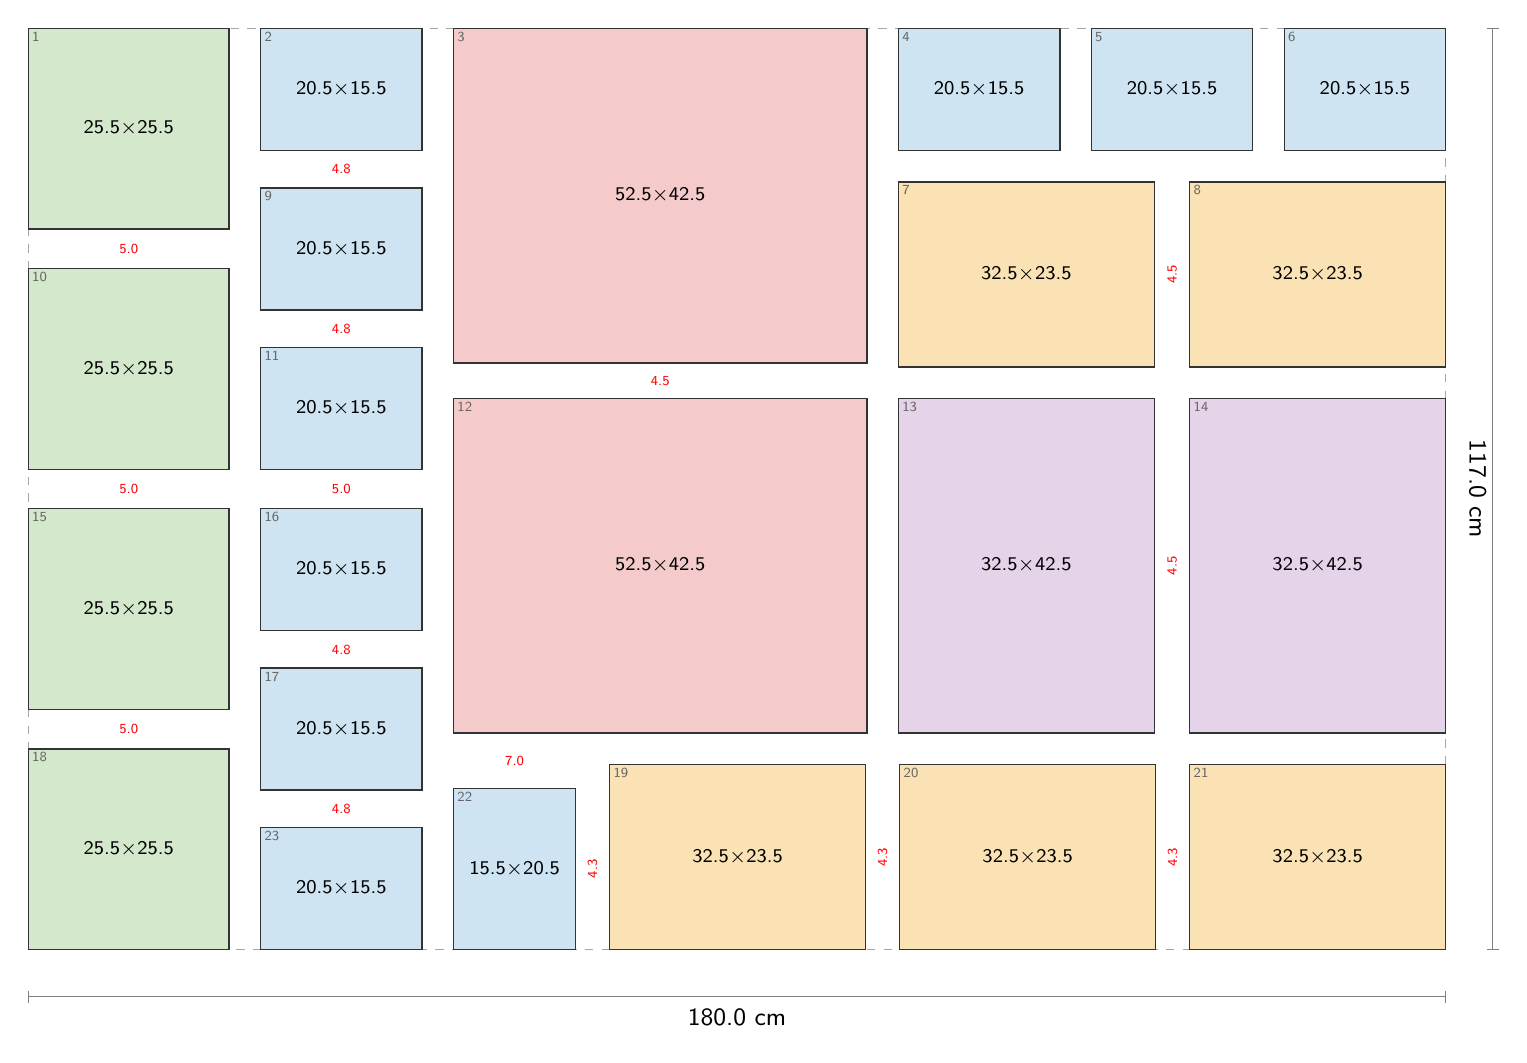
\begin{tikzpicture}[x=1mm, y=-1mm]
\draw[gray!70, dashed, line width=0.4pt] (0,0) rectangle (180.00,117.00);
\filldraw[fill=ft2, draw=black!80, line width=0.5pt] (0.00,0.00) rectangle (25.50,25.50);
\node[align=center, inner sep=0pt] at (12.75,12.75) {\scriptsize 25.5$\times$25.5};
\node[anchor=north west, inner sep=1.2pt, font=\tiny, text=black!60] at (0.00,0.00) {1};
\filldraw[fill=ft0, draw=black!80, line width=0.5pt] (29.50,0.00) rectangle (50.00,15.50);
\node[align=center, inner sep=0pt] at (39.75,7.75) {\scriptsize 20.5$\times$15.5};
\node[anchor=north west, inner sep=1.2pt, font=\tiny, text=black!60] at (29.50,0.00) {2};
\filldraw[fill=ft4, draw=black!80, line width=0.5pt] (54.00,0.00) rectangle (106.50,42.50);
\node[align=center, inner sep=0pt] at (80.25,21.25) {\scriptsize 52.5$\times$42.5};
\node[anchor=north west, inner sep=1.2pt, font=\tiny, text=black!60] at (54.00,0.00) {3};
\filldraw[fill=ft0, draw=black!80, line width=0.5pt] (110.50,0.00) rectangle (131.00,15.50);
\node[align=center, inner sep=0pt] at (120.75,7.75) {\scriptsize 20.5$\times$15.5};
\node[anchor=north west, inner sep=1.2pt, font=\tiny, text=black!60] at (110.50,0.00) {4};
\filldraw[fill=ft0, draw=black!80, line width=0.5pt] (135.00,0.00) rectangle (155.50,15.50);
\node[align=center, inner sep=0pt] at (145.25,7.75) {\scriptsize 20.5$\times$15.5};
\node[anchor=north west, inner sep=1.2pt, font=\tiny, text=black!60] at (135.00,0.00) {5};
\filldraw[fill=ft0, draw=black!80, line width=0.5pt] (159.50,0.00) rectangle (180.00,15.50);
\node[align=center, inner sep=0pt] at (169.75,7.75) {\scriptsize 20.5$\times$15.5};
\node[anchor=north west, inner sep=1.2pt, font=\tiny, text=black!60] at (159.50,0.00) {6};
\filldraw[fill=ft1, draw=black!80, line width=0.5pt] (110.50,19.50) rectangle (143.00,43.00);
\node[align=center, inner sep=0pt] at (126.75,31.25) {\scriptsize 32.5$\times$23.5};
\node[anchor=north west, inner sep=1.2pt, font=\tiny, text=black!60] at (110.50,19.50) {7};
\filldraw[fill=ft1, draw=black!80, line width=0.5pt] (147.50,19.50) rectangle (180.00,43.00);
\node[align=center, inner sep=0pt] at (163.75,31.25) {\scriptsize 32.5$\times$23.5};
\node[anchor=north west, inner sep=1.2pt, font=\tiny, text=black!60] at (147.50,19.50) {8};
\filldraw[fill=ft0, draw=black!80, line width=0.5pt] (29.50,20.25) rectangle (50.00,35.75);
\node[align=center, inner sep=0pt] at (39.75,28.00) {\scriptsize 20.5$\times$15.5};
\node[anchor=north west, inner sep=1.2pt, font=\tiny, text=black!60] at (29.50,20.25) {9};
\filldraw[fill=ft2, draw=black!80, line width=0.5pt] (0.00,30.50) rectangle (25.50,56.00);
\node[align=center, inner sep=0pt] at (12.75,43.25) {\scriptsize 25.5$\times$25.5};
\node[anchor=north west, inner sep=1.2pt, font=\tiny, text=black!60] at (0.00,30.50) {10};
\filldraw[fill=ft0, draw=black!80, line width=0.5pt] (29.50,40.50) rectangle (50.00,56.00);
\node[align=center, inner sep=0pt] at (39.75,48.25) {\scriptsize 20.5$\times$15.5};
\node[anchor=north west, inner sep=1.2pt, font=\tiny, text=black!60] at (29.50,40.50) {11};
\filldraw[fill=ft4, draw=black!80, line width=0.5pt] (54.00,47.00) rectangle (106.50,89.50);
\node[align=center, inner sep=0pt] at (80.25,68.25) {\scriptsize 52.5$\times$42.5};
\node[anchor=north west, inner sep=1.2pt, font=\tiny, text=black!60] at (54.00,47.00) {12};
\filldraw[fill=ft3, draw=black!80, line width=0.5pt] (110.50,47.00) rectangle (143.00,89.50);
\node[align=center, inner sep=0pt] at (126.75,68.25) {\scriptsize 32.5$\times$42.5};
\node[anchor=north west, inner sep=1.2pt, font=\tiny, text=black!60] at (110.50,47.00) {13};
\filldraw[fill=ft3, draw=black!80, line width=0.5pt] (147.50,47.00) rectangle (180.00,89.50);
\node[align=center, inner sep=0pt] at (163.75,68.25) {\scriptsize 32.5$\times$42.5};
\node[anchor=north west, inner sep=1.2pt, font=\tiny, text=black!60] at (147.50,47.00) {14};
\filldraw[fill=ft2, draw=black!80, line width=0.5pt] (0.00,61.00) rectangle (25.50,86.50);
\node[align=center, inner sep=0pt] at (12.75,73.75) {\scriptsize 25.5$\times$25.5};
\node[anchor=north west, inner sep=1.2pt, font=\tiny, text=black!60] at (0.00,61.00) {15};
\filldraw[fill=ft0, draw=black!80, line width=0.5pt] (29.50,61.00) rectangle (50.00,76.50);
\node[align=center, inner sep=0pt] at (39.75,68.75) {\scriptsize 20.5$\times$15.5};
\node[anchor=north west, inner sep=1.2pt, font=\tiny, text=black!60] at (29.50,61.00) {16};
\filldraw[fill=ft0, draw=black!80, line width=0.5pt] (29.50,81.25) rectangle (50.00,96.75);
\node[align=center, inner sep=0pt] at (39.75,89.00) {\scriptsize 20.5$\times$15.5};
\node[anchor=north west, inner sep=1.2pt, font=\tiny, text=black!60] at (29.50,81.25) {17};
\filldraw[fill=ft2, draw=black!80, line width=0.5pt] (0.00,91.50) rectangle (25.50,117.00);
\node[align=center, inner sep=0pt] at (12.75,104.25) {\scriptsize 25.5$\times$25.5};
\node[anchor=north west, inner sep=1.2pt, font=\tiny, text=black!60] at (0.00,91.50) {18};
\filldraw[fill=ft1, draw=black!80, line width=0.5pt] (73.83,93.50) rectangle (106.33,117.00);
\node[align=center, inner sep=0pt] at (90.08,105.25) {\scriptsize 32.5$\times$23.5};
\node[anchor=north west, inner sep=1.2pt, font=\tiny, text=black!60] at (73.83,93.50) {19};
\filldraw[fill=ft1, draw=black!80, line width=0.5pt] (110.67,93.50) rectangle (143.17,117.00);
\node[align=center, inner sep=0pt] at (126.92,105.25) {\scriptsize 32.5$\times$23.5};
\node[anchor=north west, inner sep=1.2pt, font=\tiny, text=black!60] at (110.67,93.50) {20};
\filldraw[fill=ft1, draw=black!80, line width=0.5pt] (147.50,93.50) rectangle (180.00,117.00);
\node[align=center, inner sep=0pt] at (163.75,105.25) {\scriptsize 32.5$\times$23.5};
\node[anchor=north west, inner sep=1.2pt, font=\tiny, text=black!60] at (147.50,93.50) {21};
\filldraw[fill=ft0, draw=black!80, line width=0.5pt] (54.00,96.50) rectangle (69.50,117.00);
\node[align=center, inner sep=0pt] at (61.75,106.75) {\scriptsize 15.5$\times$20.5};
\node[anchor=north west, inner sep=1.2pt, font=\tiny, text=black!60] at (54.00,96.50) {22};
\filldraw[fill=ft0, draw=black!80, line width=0.5pt] (29.50,101.50) rectangle (50.00,117.00);
\node[align=center, inner sep=0pt] at (39.75,109.25) {\scriptsize 20.5$\times$15.5};
\node[anchor=north west, inner sep=1.2pt, font=\tiny, text=black!60] at (29.50,101.50) {23};
\node[font=\tiny, text=red, fill=white, inner sep=0.3pt] at (12.75,28.00) {5.0};
\node[font=\tiny, text=red, fill=white, inner sep=0.3pt] at (39.75,17.88) {4.8};
\node[font=\tiny, text=red, fill=white, inner sep=0.3pt] at (80.25,44.75) {4.5};
\node[font=\tiny, text=red, fill=white, inner sep=0.3pt, rotate=90] at (145.25,31.25) {4.5};
\node[font=\tiny, text=red, fill=white, inner sep=0.3pt] at (39.75,38.12) {4.8};
\node[font=\tiny, text=red, fill=white, inner sep=0.3pt] at (12.75,58.50) {5.0};
\node[font=\tiny, text=red, fill=white, inner sep=0.3pt] at (39.75,58.50) {5.0};
\node[font=\tiny, text=red, fill=white, inner sep=0.3pt] at (61.75,93.00) {7.0};
\node[font=\tiny, text=red, fill=white, inner sep=0.3pt, rotate=90] at (145.25,68.25) {4.5};
\node[font=\tiny, text=red, fill=white, inner sep=0.3pt] at (12.75,89.00) {5.0};
\node[font=\tiny, text=red, fill=white, inner sep=0.3pt] at (39.75,78.88) {4.8};
\node[font=\tiny, text=red, fill=white, inner sep=0.3pt] at (39.75,99.12) {4.8};
\node[font=\tiny, text=red, fill=white, inner sep=0.3pt, rotate=90] at (108.50,105.25) {4.3};
\node[font=\tiny, text=red, fill=white, inner sep=0.3pt, rotate=90] at (145.33,105.25) {4.3};
\node[font=\tiny, text=red, fill=white, inner sep=0.3pt, rotate=90] at (71.67,106.75) {4.3};
\draw[Bar-Bar, gray] (0,123.00) -- (180.00,123.00) node[midway, below=1pt, font=\small, text=black] {180.0 cm};
\draw[Bar-Bar, gray] (186.00,0) -- (186.00,117.00) node[midway, right=1pt, font=\small, text=black, rotate=-90, anchor=north] {117.0 cm};
\end{tikzpicture}\\[4pt]
{\scriptsize Scale 1:10 (1 mm = 1 cm). Red numbers mark gaps that deviate from the nominal gap by more than 0.25 cm. Small grey numbers index the coordinate table.}
\end{minipage}\hfill
\begin{minipage}[t]{0.25\textwidth}\vspace{0pt}
\small
\begin{tabular}{@{}l l@{}}
\toprule
Outer size & 180.0 $\times$ 117.0 cm \\
Nominal gap & 4 cm \\
Actual gaps & 4.0 -- 7.0 cm \\
Max.\ deviation & 3.0 cm \\
Mean deviation & 0.29 cm \\
Border notches & none \\
Corners filled & 4 / 4 \\
Frames used & 23 of 28 \\
\bottomrule
\end{tabular}

\vspace{8pt}
\scriptsize
\begin{tabular}{@{}c l l r r@{}}
\toprule
 & outer w $\times$ h (cm) & & used & have \\
\midrule
\tikz[baseline=-0.6ex]\fill[ft0,draw=black!60] (0,0) rectangle (1.2ex,1.2ex); & 20.5$\times$15.5 & L & 9 & 9 \\
\tikz[baseline=-0.6ex]\fill[ft0,draw=black!60] (0,0) rectangle (1.2ex,1.2ex); & 15.5$\times$20.5 & P & 1 & 2 \\
\tikz[baseline=-0.6ex]\fill[ft3,draw=black!60] (0,0) rectangle (1.2ex,1.2ex); & 32.5$\times$42.5 & P & 2 & 2 \\
\tikz[baseline=-0.6ex]\fill[ft3,draw=black!60] (0,0) rectangle (1.2ex,1.2ex); & 42.5$\times$32.5 & L & 0 & 1 \\
\tikz[baseline=-0.6ex]\fill[ft1,draw=black!60] (0,0) rectangle (1.2ex,1.2ex); & 32.5$\times$23.5 & L & 5 & 5 \\
\tikz[baseline=-0.6ex]\fill[ft1,draw=black!60] (0,0) rectangle (1.2ex,1.2ex); & 23.5$\times$32.5 & P & 0 & 1 \\
\tikz[baseline=-0.6ex]\fill[ft2,draw=black!60] (0,0) rectangle (1.2ex,1.2ex); & 25.5$\times$25.5 &  & 4 & 5 \\
\tikz[baseline=-0.6ex]\fill[ft4,draw=black!60] (0,0) rectangle (1.2ex,1.2ex); & 42.5$\times$52.5 & P & 0 & 1 \\
\tikz[baseline=-0.6ex]\fill[ft4,draw=black!60] (0,0) rectangle (1.2ex,1.2ex); & 52.5$\times$42.5 & L & 2 & 2 \\
\bottomrule
\end{tabular}

\vspace{8pt}
{\bfseries Positions} (top-left corner, cm)\\[2pt]
\tiny
\begin{tabular}{@{}r l r r@{}}
\toprule
\# & frame w $\times$ h & x & y \\
\midrule
1 & 25.5 $\times$ 25.5 & 0.0 & 0.0 \\
2 & 20.5 $\times$ 15.5 & 29.5 & 0.0 \\
3 & 52.5 $\times$ 42.5 & 54.0 & 0.0 \\
4 & 20.5 $\times$ 15.5 & 110.5 & 0.0 \\
5 & 20.5 $\times$ 15.5 & 135.0 & 0.0 \\
6 & 20.5 $\times$ 15.5 & 159.5 & 0.0 \\
7 & 32.5 $\times$ 23.5 & 110.5 & 19.5 \\
8 & 32.5 $\times$ 23.5 & 147.5 & 19.5 \\
9 & 20.5 $\times$ 15.5 & 29.5 & 20.2 \\
10 & 25.5 $\times$ 25.5 & 0.0 & 30.5 \\
11 & 20.5 $\times$ 15.5 & 29.5 & 40.5 \\
12 & 52.5 $\times$ 42.5 & 54.0 & 47.0 \\
13 & 32.5 $\times$ 42.5 & 110.5 & 47.0 \\
14 & 32.5 $\times$ 42.5 & 147.5 & 47.0 \\
15 & 25.5 $\times$ 25.5 & 0.0 & 61.0 \\
16 & 20.5 $\times$ 15.5 & 29.5 & 61.0 \\
17 & 20.5 $\times$ 15.5 & 29.5 & 81.2 \\
18 & 25.5 $\times$ 25.5 & 0.0 & 91.5 \\
19 & 32.5 $\times$ 23.5 & 73.8 & 93.5 \\
20 & 32.5 $\times$ 23.5 & 110.7 & 93.5 \\
21 & 32.5 $\times$ 23.5 & 147.5 & 93.5 \\
22 & 15.5 $\times$ 20.5 & 54.0 & 96.5 \\
23 & 20.5 $\times$ 15.5 & 29.5 & 101.5 \\
\bottomrule
\end{tabular}
\end{minipage}
\clearpage

\begin{minipage}[t]{0.74\textwidth}\vspace{0pt}
{\LARGE\bfseries Layout 11}\hspace{1.5em}{\large 182.5 $\times$ 112.5 cm \quad gap 4.5 cm \quad 22 frames}\\[8pt]
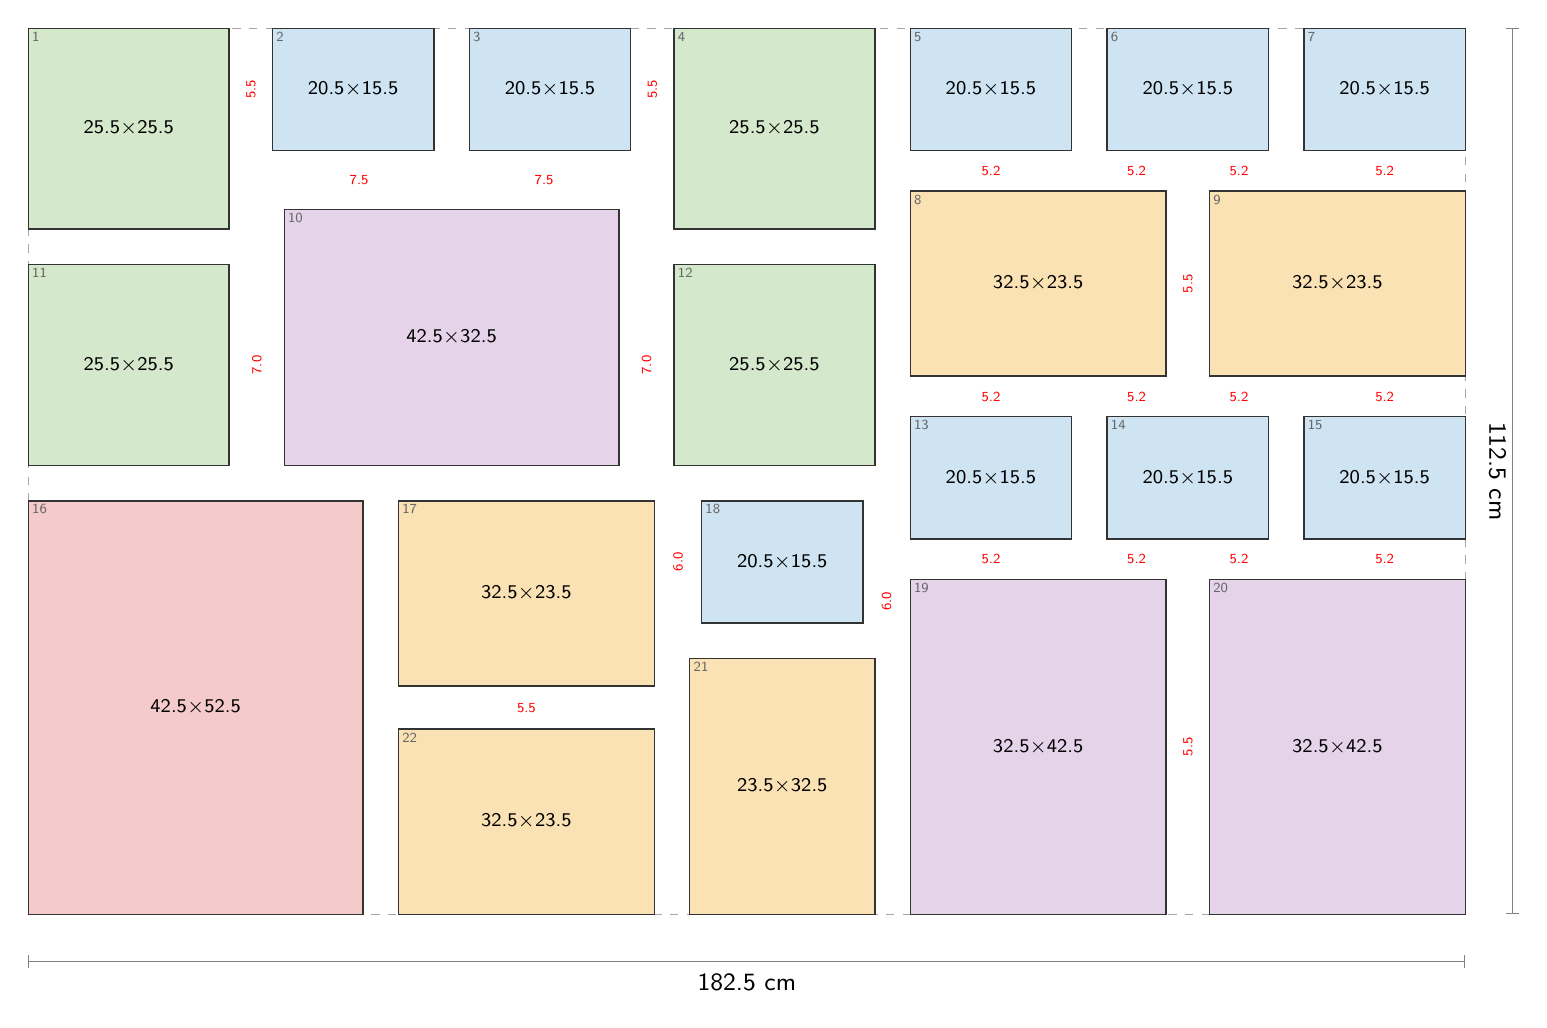
\begin{tikzpicture}[x=1mm, y=-1mm]
\draw[gray!70, dashed, line width=0.4pt] (0,0) rectangle (182.50,112.50);
\filldraw[fill=ft2, draw=black!80, line width=0.5pt] (0.00,0.00) rectangle (25.50,25.50);
\node[align=center, inner sep=0pt] at (12.75,12.75) {\scriptsize 25.5$\times$25.5};
\node[anchor=north west, inner sep=1.2pt, font=\tiny, text=black!60] at (0.00,0.00) {1};
\filldraw[fill=ft0, draw=black!80, line width=0.5pt] (31.00,0.00) rectangle (51.50,15.50);
\node[align=center, inner sep=0pt] at (41.25,7.75) {\scriptsize 20.5$\times$15.5};
\node[anchor=north west, inner sep=1.2pt, font=\tiny, text=black!60] at (31.00,0.00) {2};
\filldraw[fill=ft0, draw=black!80, line width=0.5pt] (56.00,0.00) rectangle (76.50,15.50);
\node[align=center, inner sep=0pt] at (66.25,7.75) {\scriptsize 20.5$\times$15.5};
\node[anchor=north west, inner sep=1.2pt, font=\tiny, text=black!60] at (56.00,0.00) {3};
\filldraw[fill=ft2, draw=black!80, line width=0.5pt] (82.00,0.00) rectangle (107.50,25.50);
\node[align=center, inner sep=0pt] at (94.75,12.75) {\scriptsize 25.5$\times$25.5};
\node[anchor=north west, inner sep=1.2pt, font=\tiny, text=black!60] at (82.00,0.00) {4};
\filldraw[fill=ft0, draw=black!80, line width=0.5pt] (112.00,0.00) rectangle (132.50,15.50);
\node[align=center, inner sep=0pt] at (122.25,7.75) {\scriptsize 20.5$\times$15.5};
\node[anchor=north west, inner sep=1.2pt, font=\tiny, text=black!60] at (112.00,0.00) {5};
\filldraw[fill=ft0, draw=black!80, line width=0.5pt] (137.00,0.00) rectangle (157.50,15.50);
\node[align=center, inner sep=0pt] at (147.25,7.75) {\scriptsize 20.5$\times$15.5};
\node[anchor=north west, inner sep=1.2pt, font=\tiny, text=black!60] at (137.00,0.00) {6};
\filldraw[fill=ft0, draw=black!80, line width=0.5pt] (162.00,0.00) rectangle (182.50,15.50);
\node[align=center, inner sep=0pt] at (172.25,7.75) {\scriptsize 20.5$\times$15.5};
\node[anchor=north west, inner sep=1.2pt, font=\tiny, text=black!60] at (162.00,0.00) {7};
\filldraw[fill=ft1, draw=black!80, line width=0.5pt] (112.00,20.67) rectangle (144.50,44.17);
\node[align=center, inner sep=0pt] at (128.25,32.42) {\scriptsize 32.5$\times$23.5};
\node[anchor=north west, inner sep=1.2pt, font=\tiny, text=black!60] at (112.00,20.67) {8};
\filldraw[fill=ft1, draw=black!80, line width=0.5pt] (150.00,20.67) rectangle (182.50,44.17);
\node[align=center, inner sep=0pt] at (166.25,32.42) {\scriptsize 32.5$\times$23.5};
\node[anchor=north west, inner sep=1.2pt, font=\tiny, text=black!60] at (150.00,20.67) {9};
\filldraw[fill=ft3, draw=black!80, line width=0.5pt] (32.50,23.00) rectangle (75.00,55.50);
\node[align=center, inner sep=0pt] at (53.75,39.25) {\scriptsize 42.5$\times$32.5};
\node[anchor=north west, inner sep=1.2pt, font=\tiny, text=black!60] at (32.50,23.00) {10};
\filldraw[fill=ft2, draw=black!80, line width=0.5pt] (0.00,30.00) rectangle (25.50,55.50);
\node[align=center, inner sep=0pt] at (12.75,42.75) {\scriptsize 25.5$\times$25.5};
\node[anchor=north west, inner sep=1.2pt, font=\tiny, text=black!60] at (0.00,30.00) {11};
\filldraw[fill=ft2, draw=black!80, line width=0.5pt] (82.00,30.00) rectangle (107.50,55.50);
\node[align=center, inner sep=0pt] at (94.75,42.75) {\scriptsize 25.5$\times$25.5};
\node[anchor=north west, inner sep=1.2pt, font=\tiny, text=black!60] at (82.00,30.00) {12};
\filldraw[fill=ft0, draw=black!80, line width=0.5pt] (112.00,49.33) rectangle (132.50,64.83);
\node[align=center, inner sep=0pt] at (122.25,57.08) {\scriptsize 20.5$\times$15.5};
\node[anchor=north west, inner sep=1.2pt, font=\tiny, text=black!60] at (112.00,49.33) {13};
\filldraw[fill=ft0, draw=black!80, line width=0.5pt] (137.00,49.33) rectangle (157.50,64.83);
\node[align=center, inner sep=0pt] at (147.25,57.08) {\scriptsize 20.5$\times$15.5};
\node[anchor=north west, inner sep=1.2pt, font=\tiny, text=black!60] at (137.00,49.33) {14};
\filldraw[fill=ft0, draw=black!80, line width=0.5pt] (162.00,49.33) rectangle (182.50,64.83);
\node[align=center, inner sep=0pt] at (172.25,57.08) {\scriptsize 20.5$\times$15.5};
\node[anchor=north west, inner sep=1.2pt, font=\tiny, text=black!60] at (162.00,49.33) {15};
\filldraw[fill=ft4, draw=black!80, line width=0.5pt] (0.00,60.00) rectangle (42.50,112.50);
\node[align=center, inner sep=0pt] at (21.25,86.25) {\scriptsize 42.5$\times$52.5};
\node[anchor=north west, inner sep=1.2pt, font=\tiny, text=black!60] at (0.00,60.00) {16};
\filldraw[fill=ft1, draw=black!80, line width=0.5pt] (47.00,60.00) rectangle (79.50,83.50);
\node[align=center, inner sep=0pt] at (63.25,71.75) {\scriptsize 32.5$\times$23.5};
\node[anchor=north west, inner sep=1.2pt, font=\tiny, text=black!60] at (47.00,60.00) {17};
\filldraw[fill=ft0, draw=black!80, line width=0.5pt] (85.50,60.00) rectangle (106.00,75.50);
\node[align=center, inner sep=0pt] at (95.75,67.75) {\scriptsize 20.5$\times$15.5};
\node[anchor=north west, inner sep=1.2pt, font=\tiny, text=black!60] at (85.50,60.00) {18};
\filldraw[fill=ft3, draw=black!80, line width=0.5pt] (112.00,70.00) rectangle (144.50,112.50);
\node[align=center, inner sep=0pt] at (128.25,91.25) {\scriptsize 32.5$\times$42.5};
\node[anchor=north west, inner sep=1.2pt, font=\tiny, text=black!60] at (112.00,70.00) {19};
\filldraw[fill=ft3, draw=black!80, line width=0.5pt] (150.00,70.00) rectangle (182.50,112.50);
\node[align=center, inner sep=0pt] at (166.25,91.25) {\scriptsize 32.5$\times$42.5};
\node[anchor=north west, inner sep=1.2pt, font=\tiny, text=black!60] at (150.00,70.00) {20};
\filldraw[fill=ft1, draw=black!80, line width=0.5pt] (84.00,80.00) rectangle (107.50,112.50);
\node[align=center, inner sep=0pt] at (95.75,96.25) {\scriptsize 23.5$\times$32.5};
\node[anchor=north west, inner sep=1.2pt, font=\tiny, text=black!60] at (84.00,80.00) {21};
\filldraw[fill=ft1, draw=black!80, line width=0.5pt] (47.00,89.00) rectangle (79.50,112.50);
\node[align=center, inner sep=0pt] at (63.25,100.75) {\scriptsize 32.5$\times$23.5};
\node[anchor=north west, inner sep=1.2pt, font=\tiny, text=black!60] at (47.00,89.00) {22};
\node[font=\tiny, text=red, fill=white, inner sep=0.3pt, rotate=90] at (28.25,7.75) {5.5};
\node[font=\tiny, text=red, fill=white, inner sep=0.3pt] at (42.00,19.25) {7.5};
\node[font=\tiny, text=red, fill=white, inner sep=0.3pt, rotate=90] at (79.25,7.75) {5.5};
\node[font=\tiny, text=red, fill=white, inner sep=0.3pt] at (65.50,19.25) {7.5};
\node[font=\tiny, text=red, fill=white, inner sep=0.3pt] at (122.25,18.08) {5.2};
\node[font=\tiny, text=red, fill=white, inner sep=0.3pt] at (140.75,18.08) {5.2};
\node[font=\tiny, text=red, fill=white, inner sep=0.3pt] at (153.75,18.08) {5.2};
\node[font=\tiny, text=red, fill=white, inner sep=0.3pt] at (172.25,18.08) {5.2};
\node[font=\tiny, text=red, fill=white, inner sep=0.3pt, rotate=90] at (147.25,32.42) {5.5};
\node[font=\tiny, text=red, fill=white, inner sep=0.3pt] at (122.25,46.75) {5.2};
\node[font=\tiny, text=red, fill=white, inner sep=0.3pt] at (140.75,46.75) {5.2};
\node[font=\tiny, text=red, fill=white, inner sep=0.3pt] at (153.75,46.75) {5.2};
\node[font=\tiny, text=red, fill=white, inner sep=0.3pt] at (172.25,46.75) {5.2};
\node[font=\tiny, text=red, fill=white, inner sep=0.3pt, rotate=90] at (78.50,42.75) {7.0};
\node[font=\tiny, text=red, fill=white, inner sep=0.3pt, rotate=90] at (29.00,42.75) {7.0};
\node[font=\tiny, text=red, fill=white, inner sep=0.3pt] at (122.25,67.42) {5.2};
\node[font=\tiny, text=red, fill=white, inner sep=0.3pt] at (140.75,67.42) {5.2};
\node[font=\tiny, text=red, fill=white, inner sep=0.3pt] at (153.75,67.42) {5.2};
\node[font=\tiny, text=red, fill=white, inner sep=0.3pt] at (172.25,67.42) {5.2};
\node[font=\tiny, text=red, fill=white, inner sep=0.3pt, rotate=90] at (82.50,67.75) {6.0};
\node[font=\tiny, text=red, fill=white, inner sep=0.3pt] at (63.25,86.25) {5.5};
\node[font=\tiny, text=red, fill=white, inner sep=0.3pt, rotate=90] at (109.00,72.75) {6.0};
\node[font=\tiny, text=red, fill=white, inner sep=0.3pt, rotate=90] at (147.25,91.25) {5.5};
\draw[Bar-Bar, gray] (0,118.50) -- (182.50,118.50) node[midway, below=1pt, font=\small, text=black] {182.5 cm};
\draw[Bar-Bar, gray] (188.50,0) -- (188.50,112.50) node[midway, right=1pt, font=\small, text=black, rotate=-90, anchor=north] {112.5 cm};
\end{tikzpicture}\\[4pt]
{\scriptsize Scale 1:10 (1 mm = 1 cm). Red numbers mark gaps that deviate from the nominal gap by more than 0.25 cm. Small grey numbers index the coordinate table.}
\end{minipage}\hfill
\begin{minipage}[t]{0.25\textwidth}\vspace{0pt}
\small
\begin{tabular}{@{}l l@{}}
\toprule
Outer size & 182.5 $\times$ 112.5 cm \\
Nominal gap & 4.5 cm \\
Actual gaps & 4.5 -- 7.5 cm \\
Max.\ deviation & 3.0 cm \\
Mean deviation & 0.64 cm \\
Border notches & none \\
Corners filled & 4 / 4 \\
Frames used & 22 of 28 \\
\bottomrule
\end{tabular}

\vspace{8pt}
\scriptsize
\begin{tabular}{@{}c l l r r@{}}
\toprule
 & outer w $\times$ h (cm) & & used & have \\
\midrule
\tikz[baseline=-0.6ex]\fill[ft0,draw=black!60] (0,0) rectangle (1.2ex,1.2ex); & 20.5$\times$15.5 & L & 9 & 9 \\
\tikz[baseline=-0.6ex]\fill[ft0,draw=black!60] (0,0) rectangle (1.2ex,1.2ex); & 15.5$\times$20.5 & P & 0 & 2 \\
\tikz[baseline=-0.6ex]\fill[ft3,draw=black!60] (0,0) rectangle (1.2ex,1.2ex); & 32.5$\times$42.5 & P & 2 & 2 \\
\tikz[baseline=-0.6ex]\fill[ft3,draw=black!60] (0,0) rectangle (1.2ex,1.2ex); & 42.5$\times$32.5 & L & 1 & 1 \\
\tikz[baseline=-0.6ex]\fill[ft1,draw=black!60] (0,0) rectangle (1.2ex,1.2ex); & 32.5$\times$23.5 & L & 4 & 5 \\
\tikz[baseline=-0.6ex]\fill[ft1,draw=black!60] (0,0) rectangle (1.2ex,1.2ex); & 23.5$\times$32.5 & P & 1 & 1 \\
\tikz[baseline=-0.6ex]\fill[ft2,draw=black!60] (0,0) rectangle (1.2ex,1.2ex); & 25.5$\times$25.5 &  & 4 & 5 \\
\tikz[baseline=-0.6ex]\fill[ft4,draw=black!60] (0,0) rectangle (1.2ex,1.2ex); & 42.5$\times$52.5 & P & 1 & 1 \\
\tikz[baseline=-0.6ex]\fill[ft4,draw=black!60] (0,0) rectangle (1.2ex,1.2ex); & 52.5$\times$42.5 & L & 0 & 2 \\
\bottomrule
\end{tabular}

\vspace{8pt}
{\bfseries Positions} (top-left corner, cm)\\[2pt]
\tiny
\begin{tabular}{@{}r l r r@{}}
\toprule
\# & frame w $\times$ h & x & y \\
\midrule
1 & 25.5 $\times$ 25.5 & 0.0 & 0.0 \\
2 & 20.5 $\times$ 15.5 & 31.0 & 0.0 \\
3 & 20.5 $\times$ 15.5 & 56.0 & 0.0 \\
4 & 25.5 $\times$ 25.5 & 82.0 & 0.0 \\
5 & 20.5 $\times$ 15.5 & 112.0 & 0.0 \\
6 & 20.5 $\times$ 15.5 & 137.0 & 0.0 \\
7 & 20.5 $\times$ 15.5 & 162.0 & 0.0 \\
8 & 32.5 $\times$ 23.5 & 112.0 & 20.7 \\
9 & 32.5 $\times$ 23.5 & 150.0 & 20.7 \\
10 & 42.5 $\times$ 32.5 & 32.5 & 23.0 \\
11 & 25.5 $\times$ 25.5 & 0.0 & 30.0 \\
12 & 25.5 $\times$ 25.5 & 82.0 & 30.0 \\
13 & 20.5 $\times$ 15.5 & 112.0 & 49.3 \\
14 & 20.5 $\times$ 15.5 & 137.0 & 49.3 \\
15 & 20.5 $\times$ 15.5 & 162.0 & 49.3 \\
16 & 42.5 $\times$ 52.5 & 0.0 & 60.0 \\
17 & 32.5 $\times$ 23.5 & 47.0 & 60.0 \\
18 & 20.5 $\times$ 15.5 & 85.5 & 60.0 \\
19 & 32.5 $\times$ 42.5 & 112.0 & 70.0 \\
20 & 32.5 $\times$ 42.5 & 150.0 & 70.0 \\
21 & 23.5 $\times$ 32.5 & 84.0 & 80.0 \\
22 & 32.5 $\times$ 23.5 & 47.0 & 89.0 \\
\bottomrule
\end{tabular}
\end{minipage}
\clearpage

\begin{minipage}[t]{0.74\textwidth}\vspace{0pt}
{\LARGE\bfseries Layout 12}\hspace{1.5em}{\large 170.5 $\times$ 114.5 cm \quad gap 2 cm \quad 22 frames}\\[8pt]
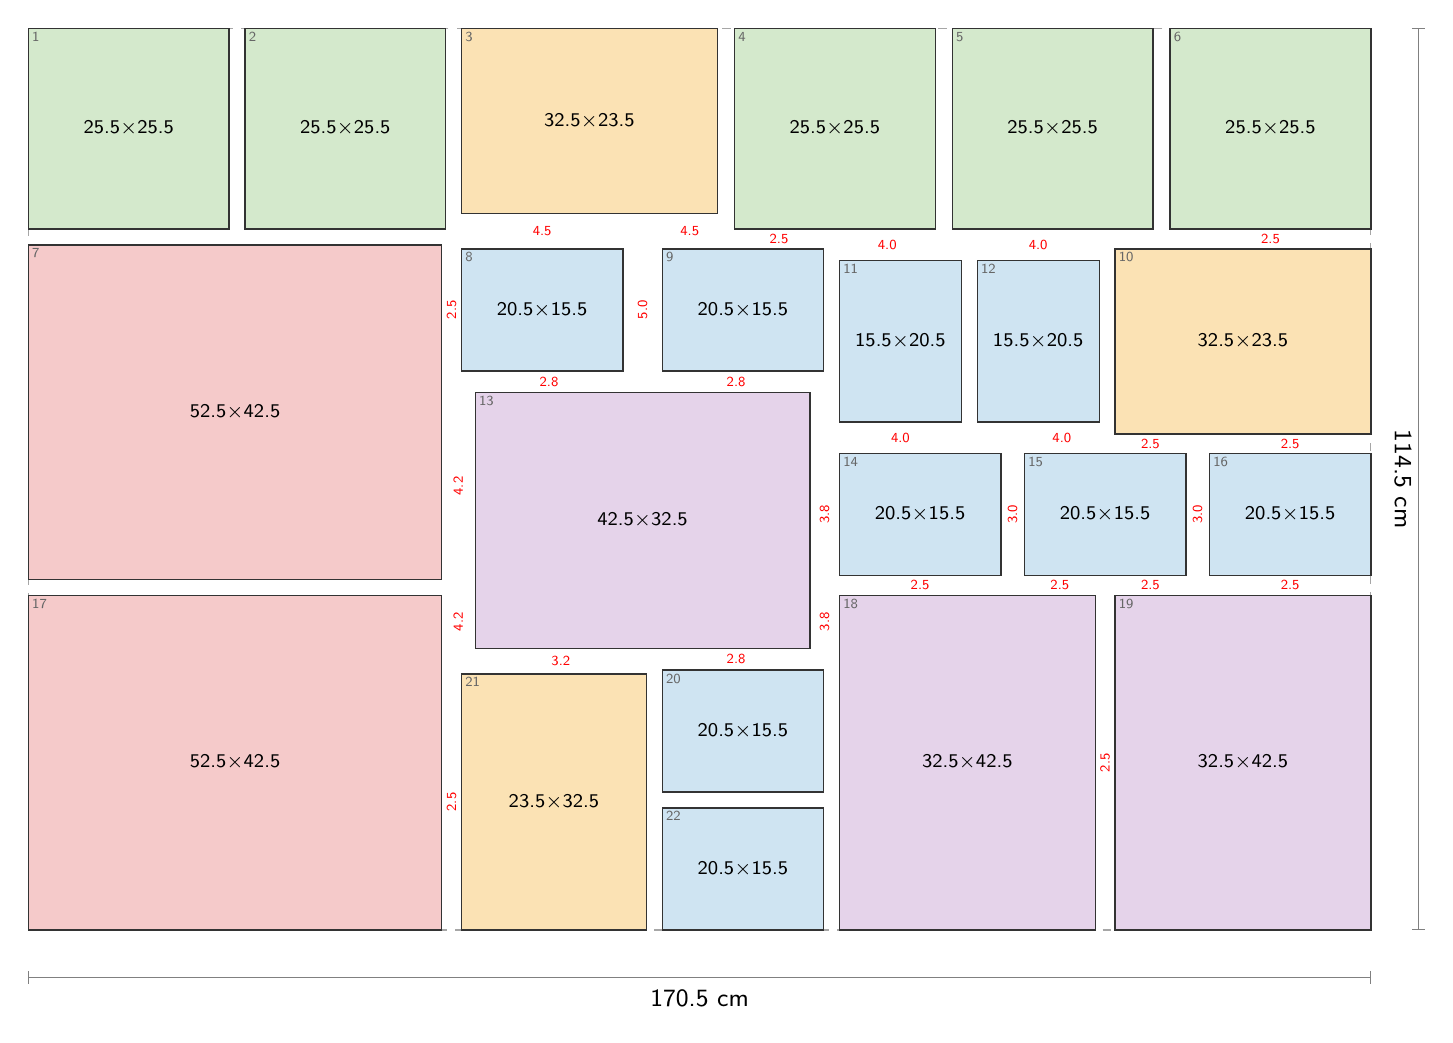
\begin{tikzpicture}[x=1mm, y=-1mm]
\draw[gray!70, dashed, line width=0.4pt] (0,0) rectangle (170.50,114.50);
\filldraw[fill=ft2, draw=black!80, line width=0.5pt] (0.00,0.00) rectangle (25.50,25.50);
\node[align=center, inner sep=0pt] at (12.75,12.75) {\scriptsize 25.5$\times$25.5};
\node[anchor=north west, inner sep=1.2pt, font=\tiny, text=black!60] at (0.00,0.00) {1};
\filldraw[fill=ft2, draw=black!80, line width=0.5pt] (27.50,0.00) rectangle (53.00,25.50);
\node[align=center, inner sep=0pt] at (40.25,12.75) {\scriptsize 25.5$\times$25.5};
\node[anchor=north west, inner sep=1.2pt, font=\tiny, text=black!60] at (27.50,0.00) {2};
\filldraw[fill=ft1, draw=black!80, line width=0.5pt] (55.00,0.00) rectangle (87.50,23.50);
\node[align=center, inner sep=0pt] at (71.25,11.75) {\scriptsize 32.5$\times$23.5};
\node[anchor=north west, inner sep=1.2pt, font=\tiny, text=black!60] at (55.00,0.00) {3};
\filldraw[fill=ft2, draw=black!80, line width=0.5pt] (89.67,0.00) rectangle (115.17,25.50);
\node[align=center, inner sep=0pt] at (102.42,12.75) {\scriptsize 25.5$\times$25.5};
\node[anchor=north west, inner sep=1.2pt, font=\tiny, text=black!60] at (89.67,0.00) {4};
\filldraw[fill=ft2, draw=black!80, line width=0.5pt] (117.33,0.00) rectangle (142.83,25.50);
\node[align=center, inner sep=0pt] at (130.08,12.75) {\scriptsize 25.5$\times$25.5};
\node[anchor=north west, inner sep=1.2pt, font=\tiny, text=black!60] at (117.33,0.00) {5};
\filldraw[fill=ft2, draw=black!80, line width=0.5pt] (145.00,0.00) rectangle (170.50,25.50);
\node[align=center, inner sep=0pt] at (157.75,12.75) {\scriptsize 25.5$\times$25.5};
\node[anchor=north west, inner sep=1.2pt, font=\tiny, text=black!60] at (145.00,0.00) {6};
\filldraw[fill=ft4, draw=black!80, line width=0.5pt] (0.00,27.50) rectangle (52.50,70.00);
\node[align=center, inner sep=0pt] at (26.25,48.75) {\scriptsize 52.5$\times$42.5};
\node[anchor=north west, inner sep=1.2pt, font=\tiny, text=black!60] at (0.00,27.50) {7};
\filldraw[fill=ft0, draw=black!80, line width=0.5pt] (55.00,28.00) rectangle (75.50,43.50);
\node[align=center, inner sep=0pt] at (65.25,35.75) {\scriptsize 20.5$\times$15.5};
\node[anchor=north west, inner sep=1.2pt, font=\tiny, text=black!60] at (55.00,28.00) {8};
\filldraw[fill=ft0, draw=black!80, line width=0.5pt] (80.50,28.00) rectangle (101.00,43.50);
\node[align=center, inner sep=0pt] at (90.75,35.75) {\scriptsize 20.5$\times$15.5};
\node[anchor=north west, inner sep=1.2pt, font=\tiny, text=black!60] at (80.50,28.00) {9};
\filldraw[fill=ft1, draw=black!80, line width=0.5pt] (138.00,28.00) rectangle (170.50,51.50);
\node[align=center, inner sep=0pt] at (154.25,39.75) {\scriptsize 32.5$\times$23.5};
\node[anchor=north west, inner sep=1.2pt, font=\tiny, text=black!60] at (138.00,28.00) {10};
\filldraw[fill=ft0, draw=black!80, line width=0.5pt] (103.00,29.50) rectangle (118.50,50.00);
\node[align=center, inner sep=0pt] at (110.75,39.75) {\scriptsize 15.5$\times$20.5};
\node[anchor=north west, inner sep=1.2pt, font=\tiny, text=black!60] at (103.00,29.50) {11};
\filldraw[fill=ft0, draw=black!80, line width=0.5pt] (120.50,29.50) rectangle (136.00,50.00);
\node[align=center, inner sep=0pt] at (128.25,39.75) {\scriptsize 15.5$\times$20.5};
\node[anchor=north west, inner sep=1.2pt, font=\tiny, text=black!60] at (120.50,29.50) {12};
\filldraw[fill=ft3, draw=black!80, line width=0.5pt] (56.75,46.25) rectangle (99.25,78.75);
\node[align=center, inner sep=0pt] at (78.00,62.50) {\scriptsize 42.5$\times$32.5};
\node[anchor=north west, inner sep=1.2pt, font=\tiny, text=black!60] at (56.75,46.25) {13};
\filldraw[fill=ft0, draw=black!80, line width=0.5pt] (103.00,54.00) rectangle (123.50,69.50);
\node[align=center, inner sep=0pt] at (113.25,61.75) {\scriptsize 20.5$\times$15.5};
\node[anchor=north west, inner sep=1.2pt, font=\tiny, text=black!60] at (103.00,54.00) {14};
\filldraw[fill=ft0, draw=black!80, line width=0.5pt] (126.50,54.00) rectangle (147.00,69.50);
\node[align=center, inner sep=0pt] at (136.75,61.75) {\scriptsize 20.5$\times$15.5};
\node[anchor=north west, inner sep=1.2pt, font=\tiny, text=black!60] at (126.50,54.00) {15};
\filldraw[fill=ft0, draw=black!80, line width=0.5pt] (150.00,54.00) rectangle (170.50,69.50);
\node[align=center, inner sep=0pt] at (160.25,61.75) {\scriptsize 20.5$\times$15.5};
\node[anchor=north west, inner sep=1.2pt, font=\tiny, text=black!60] at (150.00,54.00) {16};
\filldraw[fill=ft4, draw=black!80, line width=0.5pt] (0.00,72.00) rectangle (52.50,114.50);
\node[align=center, inner sep=0pt] at (26.25,93.25) {\scriptsize 52.5$\times$42.5};
\node[anchor=north west, inner sep=1.2pt, font=\tiny, text=black!60] at (0.00,72.00) {17};
\filldraw[fill=ft3, draw=black!80, line width=0.5pt] (103.00,72.00) rectangle (135.50,114.50);
\node[align=center, inner sep=0pt] at (119.25,93.25) {\scriptsize 32.5$\times$42.5};
\node[anchor=north west, inner sep=1.2pt, font=\tiny, text=black!60] at (103.00,72.00) {18};
\filldraw[fill=ft3, draw=black!80, line width=0.5pt] (138.00,72.00) rectangle (170.50,114.50);
\node[align=center, inner sep=0pt] at (154.25,93.25) {\scriptsize 32.5$\times$42.5};
\node[anchor=north west, inner sep=1.2pt, font=\tiny, text=black!60] at (138.00,72.00) {19};
\filldraw[fill=ft0, draw=black!80, line width=0.5pt] (80.50,81.50) rectangle (101.00,97.00);
\node[align=center, inner sep=0pt] at (90.75,89.25) {\scriptsize 20.5$\times$15.5};
\node[anchor=north west, inner sep=1.2pt, font=\tiny, text=black!60] at (80.50,81.50) {20};
\filldraw[fill=ft1, draw=black!80, line width=0.5pt] (55.00,82.00) rectangle (78.50,114.50);
\node[align=center, inner sep=0pt] at (66.75,98.25) {\scriptsize 23.5$\times$32.5};
\node[anchor=north west, inner sep=1.2pt, font=\tiny, text=black!60] at (55.00,82.00) {21};
\filldraw[fill=ft0, draw=black!80, line width=0.5pt] (80.50,99.00) rectangle (101.00,114.50);
\node[align=center, inner sep=0pt] at (90.75,106.75) {\scriptsize 20.5$\times$15.5};
\node[anchor=north west, inner sep=1.2pt, font=\tiny, text=black!60] at (80.50,99.00) {22};
\node[font=\tiny, text=red, fill=white, inner sep=0.3pt] at (65.25,25.75) {4.5};
\node[font=\tiny, text=red, fill=white, inner sep=0.3pt] at (84.00,25.75) {4.5};
\node[font=\tiny, text=red, fill=white, inner sep=0.3pt] at (95.33,26.75) {2.5};
\node[font=\tiny, text=red, fill=white, inner sep=0.3pt] at (109.08,27.50) {4.0};
\node[font=\tiny, text=red, fill=white, inner sep=0.3pt] at (128.25,27.50) {4.0};
\node[font=\tiny, text=red, fill=white, inner sep=0.3pt] at (157.75,26.75) {2.5};
\node[font=\tiny, text=red, fill=white, inner sep=0.3pt, rotate=90] at (53.75,35.75) {2.5};
\node[font=\tiny, text=red, fill=white, inner sep=0.3pt, rotate=90] at (54.62,58.12) {4.2};
\node[font=\tiny, text=red, fill=white, inner sep=0.3pt, rotate=90] at (78.00,35.75) {5.0};
\node[font=\tiny, text=red, fill=white, inner sep=0.3pt] at (66.12,44.88) {2.8};
\node[font=\tiny, text=red, fill=white, inner sep=0.3pt] at (89.88,44.88) {2.8};
\node[font=\tiny, text=red, fill=white, inner sep=0.3pt] at (142.50,52.75) {2.5};
\node[font=\tiny, text=red, fill=white, inner sep=0.3pt] at (160.25,52.75) {2.5};
\node[font=\tiny, text=red, fill=white, inner sep=0.3pt] at (110.75,52.00) {4.0};
\node[font=\tiny, text=red, fill=white, inner sep=0.3pt] at (131.25,52.00) {4.0};
\node[font=\tiny, text=red, fill=white, inner sep=0.3pt, rotate=90] at (101.12,61.75) {3.8};
\node[font=\tiny, text=red, fill=white, inner sep=0.3pt, rotate=90] at (101.12,75.38) {3.8};
\node[font=\tiny, text=red, fill=white, inner sep=0.3pt] at (89.88,80.12) {2.8};
\node[font=\tiny, text=red, fill=white, inner sep=0.3pt] at (67.62,80.38) {3.2};
\node[font=\tiny, text=red, fill=white, inner sep=0.3pt, rotate=90] at (125.00,61.75) {3.0};
\node[font=\tiny, text=red, fill=white, inner sep=0.3pt] at (113.25,70.75) {2.5};
\node[font=\tiny, text=red, fill=white, inner sep=0.3pt, rotate=90] at (148.50,61.75) {3.0};
\node[font=\tiny, text=red, fill=white, inner sep=0.3pt] at (131.00,70.75) {2.5};
\node[font=\tiny, text=red, fill=white, inner sep=0.3pt] at (142.50,70.75) {2.5};
\node[font=\tiny, text=red, fill=white, inner sep=0.3pt] at (160.25,70.75) {2.5};
\node[font=\tiny, text=red, fill=white, inner sep=0.3pt, rotate=90] at (54.62,75.38) {4.2};
\node[font=\tiny, text=red, fill=white, inner sep=0.3pt, rotate=90] at (53.75,98.25) {2.5};
\node[font=\tiny, text=red, fill=white, inner sep=0.3pt, rotate=90] at (136.75,93.25) {2.5};
\draw[Bar-Bar, gray] (0,120.50) -- (170.50,120.50) node[midway, below=1pt, font=\small, text=black] {170.5 cm};
\draw[Bar-Bar, gray] (176.50,0) -- (176.50,114.50) node[midway, right=1pt, font=\small, text=black, rotate=-90, anchor=north] {114.5 cm};
\end{tikzpicture}\\[4pt]
{\scriptsize Scale 1:10 (1 mm = 1 cm). Red numbers mark gaps that deviate from the nominal gap by more than 0.25 cm. Small grey numbers index the coordinate table.}
\end{minipage}\hfill
\begin{minipage}[t]{0.25\textwidth}\vspace{0pt}
\small
\begin{tabular}{@{}l l@{}}
\toprule
Outer size & 170.5 $\times$ 114.5 cm \\
Nominal gap & 2 cm \\
Actual gaps & 2.0 -- 5.0 cm \\
Max.\ deviation & 3.0 cm \\
Mean deviation & 0.81 cm \\
Border notches & none \\
Corners filled & 4 / 4 \\
Frames used & 22 of 28 \\
\bottomrule
\end{tabular}

\vspace{8pt}
\scriptsize
\begin{tabular}{@{}c l l r r@{}}
\toprule
 & outer w $\times$ h (cm) & & used & have \\
\midrule
\tikz[baseline=-0.6ex]\fill[ft0,draw=black!60] (0,0) rectangle (1.2ex,1.2ex); & 20.5$\times$15.5 & L & 7 & 9 \\
\tikz[baseline=-0.6ex]\fill[ft0,draw=black!60] (0,0) rectangle (1.2ex,1.2ex); & 15.5$\times$20.5 & P & 2 & 2 \\
\tikz[baseline=-0.6ex]\fill[ft3,draw=black!60] (0,0) rectangle (1.2ex,1.2ex); & 32.5$\times$42.5 & P & 2 & 2 \\
\tikz[baseline=-0.6ex]\fill[ft3,draw=black!60] (0,0) rectangle (1.2ex,1.2ex); & 42.5$\times$32.5 & L & 1 & 1 \\
\tikz[baseline=-0.6ex]\fill[ft1,draw=black!60] (0,0) rectangle (1.2ex,1.2ex); & 32.5$\times$23.5 & L & 2 & 5 \\
\tikz[baseline=-0.6ex]\fill[ft1,draw=black!60] (0,0) rectangle (1.2ex,1.2ex); & 23.5$\times$32.5 & P & 1 & 1 \\
\tikz[baseline=-0.6ex]\fill[ft2,draw=black!60] (0,0) rectangle (1.2ex,1.2ex); & 25.5$\times$25.5 &  & 5 & 5 \\
\tikz[baseline=-0.6ex]\fill[ft4,draw=black!60] (0,0) rectangle (1.2ex,1.2ex); & 42.5$\times$52.5 & P & 0 & 1 \\
\tikz[baseline=-0.6ex]\fill[ft4,draw=black!60] (0,0) rectangle (1.2ex,1.2ex); & 52.5$\times$42.5 & L & 2 & 2 \\
\bottomrule
\end{tabular}

\vspace{8pt}
{\bfseries Positions} (top-left corner, cm)\\[2pt]
\tiny
\begin{tabular}{@{}r l r r@{}}
\toprule
\# & frame w $\times$ h & x & y \\
\midrule
1 & 25.5 $\times$ 25.5 & 0.0 & 0.0 \\
2 & 25.5 $\times$ 25.5 & 27.5 & 0.0 \\
3 & 32.5 $\times$ 23.5 & 55.0 & 0.0 \\
4 & 25.5 $\times$ 25.5 & 89.7 & 0.0 \\
5 & 25.5 $\times$ 25.5 & 117.3 & 0.0 \\
6 & 25.5 $\times$ 25.5 & 145.0 & 0.0 \\
7 & 52.5 $\times$ 42.5 & 0.0 & 27.5 \\
8 & 20.5 $\times$ 15.5 & 55.0 & 28.0 \\
9 & 20.5 $\times$ 15.5 & 80.5 & 28.0 \\
10 & 32.5 $\times$ 23.5 & 138.0 & 28.0 \\
11 & 15.5 $\times$ 20.5 & 103.0 & 29.5 \\
12 & 15.5 $\times$ 20.5 & 120.5 & 29.5 \\
13 & 42.5 $\times$ 32.5 & 56.8 & 46.2 \\
14 & 20.5 $\times$ 15.5 & 103.0 & 54.0 \\
15 & 20.5 $\times$ 15.5 & 126.5 & 54.0 \\
16 & 20.5 $\times$ 15.5 & 150.0 & 54.0 \\
17 & 52.5 $\times$ 42.5 & 0.0 & 72.0 \\
18 & 32.5 $\times$ 42.5 & 103.0 & 72.0 \\
19 & 32.5 $\times$ 42.5 & 138.0 & 72.0 \\
20 & 20.5 $\times$ 15.5 & 80.5 & 81.5 \\
21 & 23.5 $\times$ 32.5 & 55.0 & 82.0 \\
22 & 20.5 $\times$ 15.5 & 80.5 & 99.0 \\
\bottomrule
\end{tabular}
\end{minipage}
\clearpage

\begin{minipage}[t]{0.74\textwidth}\vspace{0pt}
{\LARGE\bfseries Layout 13}\hspace{1.5em}{\large 177.5 $\times$ 113.5 cm \quad gap 1.5 cm \quad 21 frames}\\[8pt]
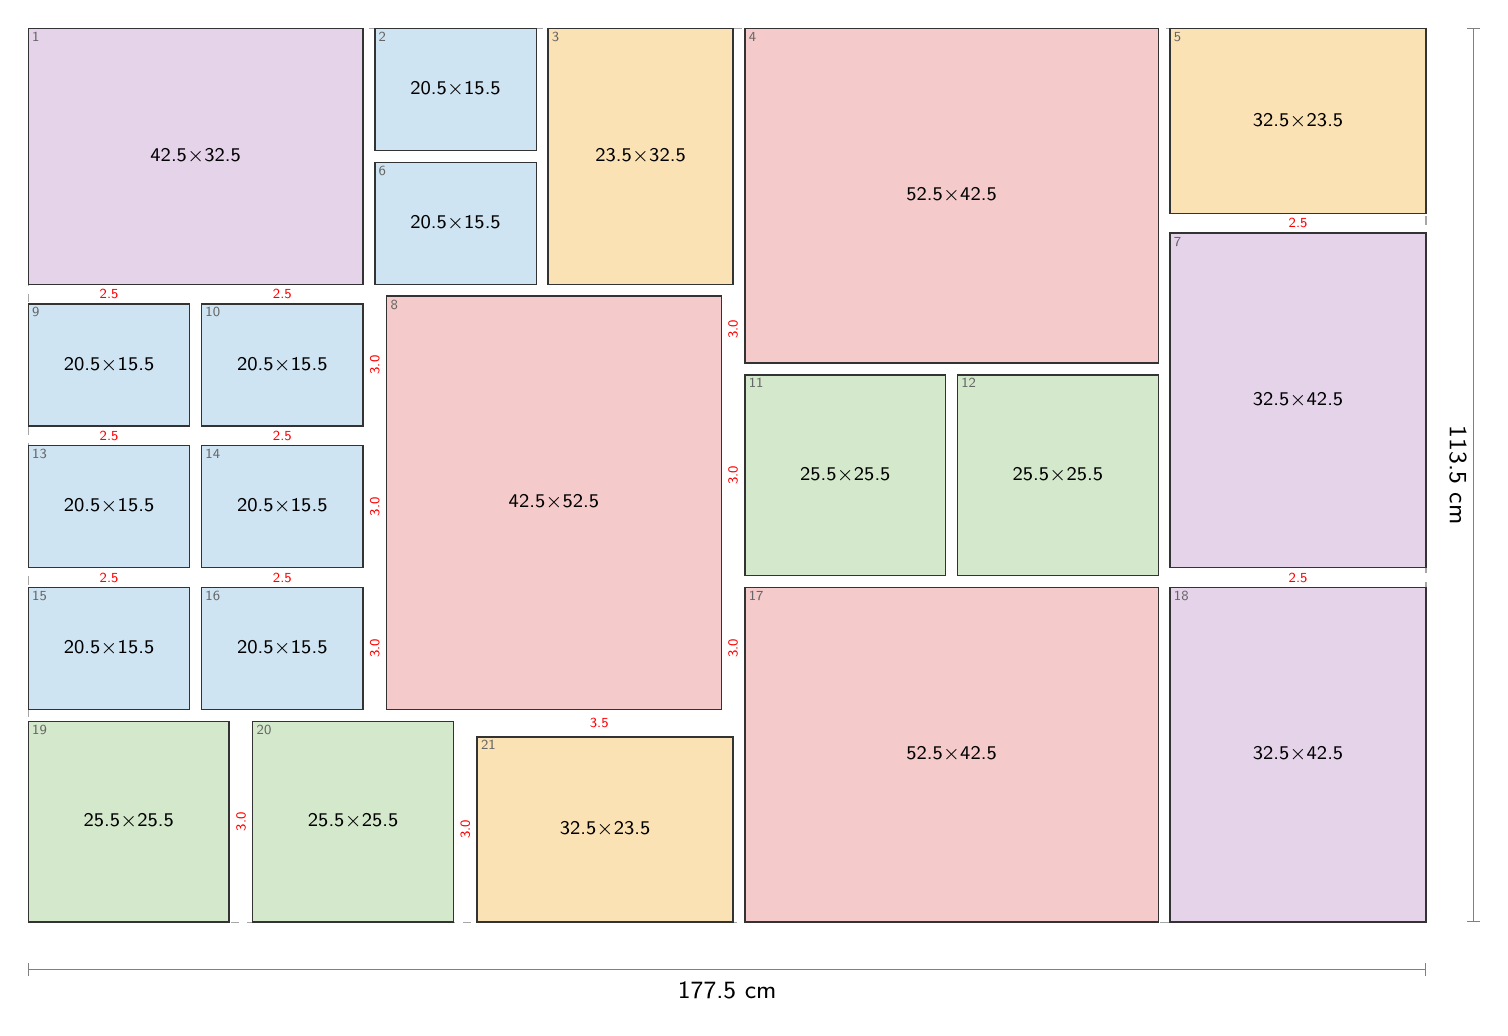
\begin{tikzpicture}[x=1mm, y=-1mm]
\draw[gray!70, dashed, line width=0.4pt] (0,0) rectangle (177.50,113.50);
\filldraw[fill=ft3, draw=black!80, line width=0.5pt] (0.00,0.00) rectangle (42.50,32.50);
\node[align=center, inner sep=0pt] at (21.25,16.25) {\scriptsize 42.5$\times$32.5};
\node[anchor=north west, inner sep=1.2pt, font=\tiny, text=black!60] at (0.00,0.00) {1};
\filldraw[fill=ft0, draw=black!80, line width=0.5pt] (44.00,0.00) rectangle (64.50,15.50);
\node[align=center, inner sep=0pt] at (54.25,7.75) {\scriptsize 20.5$\times$15.5};
\node[anchor=north west, inner sep=1.2pt, font=\tiny, text=black!60] at (44.00,0.00) {2};
\filldraw[fill=ft1, draw=black!80, line width=0.5pt] (66.00,0.00) rectangle (89.50,32.50);
\node[align=center, inner sep=0pt] at (77.75,16.25) {\scriptsize 23.5$\times$32.5};
\node[anchor=north west, inner sep=1.2pt, font=\tiny, text=black!60] at (66.00,0.00) {3};
\filldraw[fill=ft4, draw=black!80, line width=0.5pt] (91.00,0.00) rectangle (143.50,42.50);
\node[align=center, inner sep=0pt] at (117.25,21.25) {\scriptsize 52.5$\times$42.5};
\node[anchor=north west, inner sep=1.2pt, font=\tiny, text=black!60] at (91.00,0.00) {4};
\filldraw[fill=ft1, draw=black!80, line width=0.5pt] (145.00,0.00) rectangle (177.50,23.50);
\node[align=center, inner sep=0pt] at (161.25,11.75) {\scriptsize 32.5$\times$23.5};
\node[anchor=north west, inner sep=1.2pt, font=\tiny, text=black!60] at (145.00,0.00) {5};
\filldraw[fill=ft0, draw=black!80, line width=0.5pt] (44.00,17.00) rectangle (64.50,32.50);
\node[align=center, inner sep=0pt] at (54.25,24.75) {\scriptsize 20.5$\times$15.5};
\node[anchor=north west, inner sep=1.2pt, font=\tiny, text=black!60] at (44.00,17.00) {6};
\filldraw[fill=ft3, draw=black!80, line width=0.5pt] (145.00,26.00) rectangle (177.50,68.50);
\node[align=center, inner sep=0pt] at (161.25,47.25) {\scriptsize 32.5$\times$42.5};
\node[anchor=north west, inner sep=1.2pt, font=\tiny, text=black!60] at (145.00,26.00) {7};
\filldraw[fill=ft4, draw=black!80, line width=0.5pt] (45.50,34.00) rectangle (88.00,86.50);
\node[align=center, inner sep=0pt] at (66.75,60.25) {\scriptsize 42.5$\times$52.5};
\node[anchor=north west, inner sep=1.2pt, font=\tiny, text=black!60] at (45.50,34.00) {8};
\filldraw[fill=ft0, draw=black!80, line width=0.5pt] (0.00,35.00) rectangle (20.50,50.50);
\node[align=center, inner sep=0pt] at (10.25,42.75) {\scriptsize 20.5$\times$15.5};
\node[anchor=north west, inner sep=1.2pt, font=\tiny, text=black!60] at (0.00,35.00) {9};
\filldraw[fill=ft0, draw=black!80, line width=0.5pt] (22.00,35.00) rectangle (42.50,50.50);
\node[align=center, inner sep=0pt] at (32.25,42.75) {\scriptsize 20.5$\times$15.5};
\node[anchor=north west, inner sep=1.2pt, font=\tiny, text=black!60] at (22.00,35.00) {10};
\filldraw[fill=ft2, draw=black!80, line width=0.5pt] (91.00,44.00) rectangle (116.50,69.50);
\node[align=center, inner sep=0pt] at (103.75,56.75) {\scriptsize 25.5$\times$25.5};
\node[anchor=north west, inner sep=1.2pt, font=\tiny, text=black!60] at (91.00,44.00) {11};
\filldraw[fill=ft2, draw=black!80, line width=0.5pt] (118.00,44.00) rectangle (143.50,69.50);
\node[align=center, inner sep=0pt] at (130.75,56.75) {\scriptsize 25.5$\times$25.5};
\node[anchor=north west, inner sep=1.2pt, font=\tiny, text=black!60] at (118.00,44.00) {12};
\filldraw[fill=ft0, draw=black!80, line width=0.5pt] (0.00,53.00) rectangle (20.50,68.50);
\node[align=center, inner sep=0pt] at (10.25,60.75) {\scriptsize 20.5$\times$15.5};
\node[anchor=north west, inner sep=1.2pt, font=\tiny, text=black!60] at (0.00,53.00) {13};
\filldraw[fill=ft0, draw=black!80, line width=0.5pt] (22.00,53.00) rectangle (42.50,68.50);
\node[align=center, inner sep=0pt] at (32.25,60.75) {\scriptsize 20.5$\times$15.5};
\node[anchor=north west, inner sep=1.2pt, font=\tiny, text=black!60] at (22.00,53.00) {14};
\filldraw[fill=ft0, draw=black!80, line width=0.5pt] (0.00,71.00) rectangle (20.50,86.50);
\node[align=center, inner sep=0pt] at (10.25,78.75) {\scriptsize 20.5$\times$15.5};
\node[anchor=north west, inner sep=1.2pt, font=\tiny, text=black!60] at (0.00,71.00) {15};
\filldraw[fill=ft0, draw=black!80, line width=0.5pt] (22.00,71.00) rectangle (42.50,86.50);
\node[align=center, inner sep=0pt] at (32.25,78.75) {\scriptsize 20.5$\times$15.5};
\node[anchor=north west, inner sep=1.2pt, font=\tiny, text=black!60] at (22.00,71.00) {16};
\filldraw[fill=ft4, draw=black!80, line width=0.5pt] (91.00,71.00) rectangle (143.50,113.50);
\node[align=center, inner sep=0pt] at (117.25,92.25) {\scriptsize 52.5$\times$42.5};
\node[anchor=north west, inner sep=1.2pt, font=\tiny, text=black!60] at (91.00,71.00) {17};
\filldraw[fill=ft3, draw=black!80, line width=0.5pt] (145.00,71.00) rectangle (177.50,113.50);
\node[align=center, inner sep=0pt] at (161.25,92.25) {\scriptsize 32.5$\times$42.5};
\node[anchor=north west, inner sep=1.2pt, font=\tiny, text=black!60] at (145.00,71.00) {18};
\filldraw[fill=ft2, draw=black!80, line width=0.5pt] (0.00,88.00) rectangle (25.50,113.50);
\node[align=center, inner sep=0pt] at (12.75,100.75) {\scriptsize 25.5$\times$25.5};
\node[anchor=north west, inner sep=1.2pt, font=\tiny, text=black!60] at (0.00,88.00) {19};
\filldraw[fill=ft2, draw=black!80, line width=0.5pt] (28.50,88.00) rectangle (54.00,113.50);
\node[align=center, inner sep=0pt] at (41.25,100.75) {\scriptsize 25.5$\times$25.5};
\node[anchor=north west, inner sep=1.2pt, font=\tiny, text=black!60] at (28.50,88.00) {20};
\filldraw[fill=ft1, draw=black!80, line width=0.5pt] (57.00,90.00) rectangle (89.50,113.50);
\node[align=center, inner sep=0pt] at (73.25,101.75) {\scriptsize 32.5$\times$23.5};
\node[anchor=north west, inner sep=1.2pt, font=\tiny, text=black!60] at (57.00,90.00) {21};
\node[font=\tiny, text=red, fill=white, inner sep=0.3pt] at (10.25,33.75) {2.5};
\node[font=\tiny, text=red, fill=white, inner sep=0.3pt] at (32.25,33.75) {2.5};
\node[font=\tiny, text=red, fill=white, inner sep=0.3pt] at (161.25,24.75) {2.5};
\node[font=\tiny, text=red, fill=white, inner sep=0.3pt] at (161.25,69.75) {2.5};
\node[font=\tiny, text=red, fill=white, inner sep=0.3pt, rotate=90] at (89.50,38.25) {3.0};
\node[font=\tiny, text=red, fill=white, inner sep=0.3pt, rotate=90] at (89.50,56.75) {3.0};
\node[font=\tiny, text=red, fill=white, inner sep=0.3pt, rotate=90] at (89.50,78.75) {3.0};
\node[font=\tiny, text=red, fill=white, inner sep=0.3pt] at (72.50,88.25) {3.5};
\node[font=\tiny, text=red, fill=white, inner sep=0.3pt] at (10.25,51.75) {2.5};
\node[font=\tiny, text=red, fill=white, inner sep=0.3pt, rotate=90] at (44.00,42.75) {3.0};
\node[font=\tiny, text=red, fill=white, inner sep=0.3pt] at (32.25,51.75) {2.5};
\node[font=\tiny, text=red, fill=white, inner sep=0.3pt] at (10.25,69.75) {2.5};
\node[font=\tiny, text=red, fill=white, inner sep=0.3pt, rotate=90] at (44.00,60.75) {3.0};
\node[font=\tiny, text=red, fill=white, inner sep=0.3pt] at (32.25,69.75) {2.5};
\node[font=\tiny, text=red, fill=white, inner sep=0.3pt, rotate=90] at (44.00,78.75) {3.0};
\node[font=\tiny, text=red, fill=white, inner sep=0.3pt, rotate=90] at (27.00,100.75) {3.0};
\node[font=\tiny, text=red, fill=white, inner sep=0.3pt, rotate=90] at (55.50,101.75) {3.0};
\draw[Bar-Bar, gray] (0,119.50) -- (177.50,119.50) node[midway, below=1pt, font=\small, text=black] {177.5 cm};
\draw[Bar-Bar, gray] (183.50,0) -- (183.50,113.50) node[midway, right=1pt, font=\small, text=black, rotate=-90, anchor=north] {113.5 cm};
\end{tikzpicture}\\[4pt]
{\scriptsize Scale 1:10 (1 mm = 1 cm). Red numbers mark gaps that deviate from the nominal gap by more than 0.25 cm. Small grey numbers index the coordinate table.}
\end{minipage}\hfill
\begin{minipage}[t]{0.25\textwidth}\vspace{0pt}
\small
\begin{tabular}{@{}l l@{}}
\toprule
Outer size & 177.5 $\times$ 113.5 cm \\
Nominal gap & 1.5 cm \\
Actual gaps & 1.5 -- 3.5 cm \\
Max.\ deviation & 2.0 cm \\
Mean deviation & 0.54 cm \\
Border notches & bottom 6 cm \\
Corners filled & 4 / 4 \\
Frames used & 21 of 28 \\
\bottomrule
\end{tabular}

\vspace{8pt}
\scriptsize
\begin{tabular}{@{}c l l r r@{}}
\toprule
 & outer w $\times$ h (cm) & & used & have \\
\midrule
\tikz[baseline=-0.6ex]\fill[ft0,draw=black!60] (0,0) rectangle (1.2ex,1.2ex); & 20.5$\times$15.5 & L & 8 & 9 \\
\tikz[baseline=-0.6ex]\fill[ft0,draw=black!60] (0,0) rectangle (1.2ex,1.2ex); & 15.5$\times$20.5 & P & 0 & 2 \\
\tikz[baseline=-0.6ex]\fill[ft3,draw=black!60] (0,0) rectangle (1.2ex,1.2ex); & 32.5$\times$42.5 & P & 2 & 2 \\
\tikz[baseline=-0.6ex]\fill[ft3,draw=black!60] (0,0) rectangle (1.2ex,1.2ex); & 42.5$\times$32.5 & L & 1 & 1 \\
\tikz[baseline=-0.6ex]\fill[ft1,draw=black!60] (0,0) rectangle (1.2ex,1.2ex); & 32.5$\times$23.5 & L & 2 & 5 \\
\tikz[baseline=-0.6ex]\fill[ft1,draw=black!60] (0,0) rectangle (1.2ex,1.2ex); & 23.5$\times$32.5 & P & 1 & 1 \\
\tikz[baseline=-0.6ex]\fill[ft2,draw=black!60] (0,0) rectangle (1.2ex,1.2ex); & 25.5$\times$25.5 &  & 4 & 5 \\
\tikz[baseline=-0.6ex]\fill[ft4,draw=black!60] (0,0) rectangle (1.2ex,1.2ex); & 42.5$\times$52.5 & P & 1 & 1 \\
\tikz[baseline=-0.6ex]\fill[ft4,draw=black!60] (0,0) rectangle (1.2ex,1.2ex); & 52.5$\times$42.5 & L & 2 & 2 \\
\bottomrule
\end{tabular}

\vspace{8pt}
{\bfseries Positions} (top-left corner, cm)\\[2pt]
\tiny
\begin{tabular}{@{}r l r r@{}}
\toprule
\# & frame w $\times$ h & x & y \\
\midrule
1 & 42.5 $\times$ 32.5 & 0.0 & 0.0 \\
2 & 20.5 $\times$ 15.5 & 44.0 & 0.0 \\
3 & 23.5 $\times$ 32.5 & 66.0 & 0.0 \\
4 & 52.5 $\times$ 42.5 & 91.0 & 0.0 \\
5 & 32.5 $\times$ 23.5 & 145.0 & 0.0 \\
6 & 20.5 $\times$ 15.5 & 44.0 & 17.0 \\
7 & 32.5 $\times$ 42.5 & 145.0 & 26.0 \\
8 & 42.5 $\times$ 52.5 & 45.5 & 34.0 \\
9 & 20.5 $\times$ 15.5 & 0.0 & 35.0 \\
10 & 20.5 $\times$ 15.5 & 22.0 & 35.0 \\
11 & 25.5 $\times$ 25.5 & 91.0 & 44.0 \\
12 & 25.5 $\times$ 25.5 & 118.0 & 44.0 \\
13 & 20.5 $\times$ 15.5 & 0.0 & 53.0 \\
14 & 20.5 $\times$ 15.5 & 22.0 & 53.0 \\
15 & 20.5 $\times$ 15.5 & 0.0 & 71.0 \\
16 & 20.5 $\times$ 15.5 & 22.0 & 71.0 \\
17 & 52.5 $\times$ 42.5 & 91.0 & 71.0 \\
18 & 32.5 $\times$ 42.5 & 145.0 & 71.0 \\
19 & 25.5 $\times$ 25.5 & 0.0 & 88.0 \\
20 & 25.5 $\times$ 25.5 & 28.5 & 88.0 \\
21 & 32.5 $\times$ 23.5 & 57.0 & 90.0 \\
\bottomrule
\end{tabular}
\end{minipage}
\clearpage

\begin{minipage}[t]{0.74\textwidth}\vspace{0pt}
{\LARGE\bfseries Layout 14}\hspace{1.5em}{\large 171.0 $\times$ 120.5 cm \quad gap 6 cm \quad 14 frames}\\[8pt]
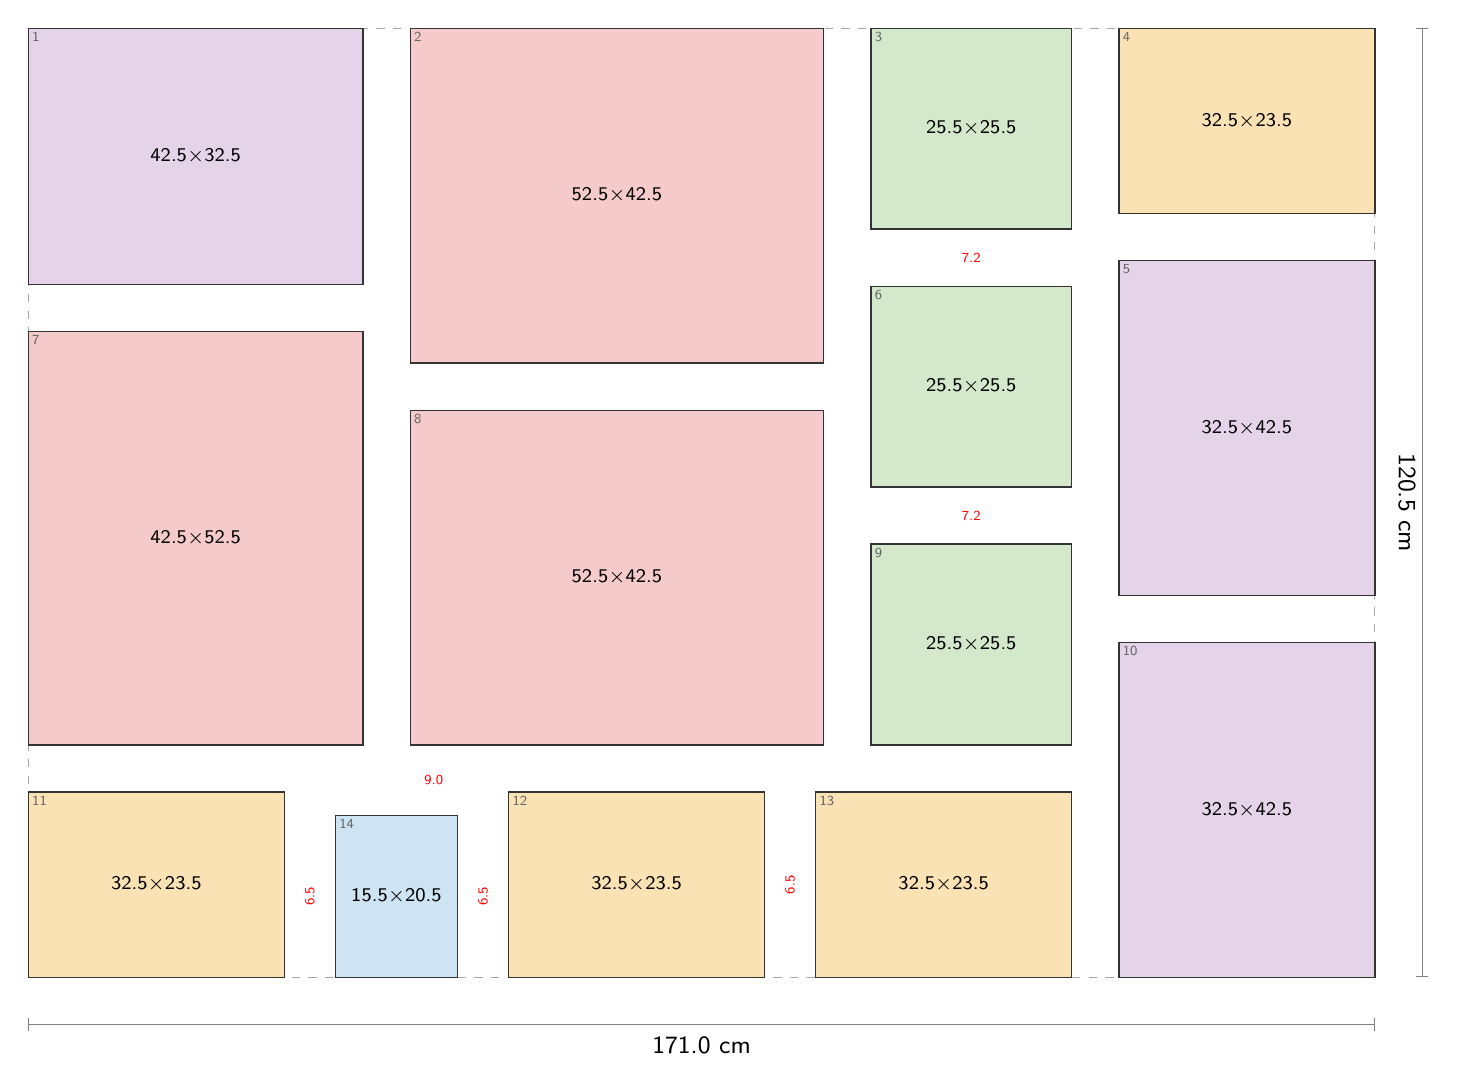
\begin{tikzpicture}[x=1mm, y=-1mm]
\draw[gray!70, dashed, line width=0.4pt] (0,0) rectangle (171.00,120.50);
\filldraw[fill=ft3, draw=black!80, line width=0.5pt] (0.00,0.00) rectangle (42.50,32.50);
\node[align=center, inner sep=0pt] at (21.25,16.25) {\scriptsize 42.5$\times$32.5};
\node[anchor=north west, inner sep=1.2pt, font=\tiny, text=black!60] at (0.00,0.00) {1};
\filldraw[fill=ft4, draw=black!80, line width=0.5pt] (48.50,0.00) rectangle (101.00,42.50);
\node[align=center, inner sep=0pt] at (74.75,21.25) {\scriptsize 52.5$\times$42.5};
\node[anchor=north west, inner sep=1.2pt, font=\tiny, text=black!60] at (48.50,0.00) {2};
\filldraw[fill=ft2, draw=black!80, line width=0.5pt] (107.00,0.00) rectangle (132.50,25.50);
\node[align=center, inner sep=0pt] at (119.75,12.75) {\scriptsize 25.5$\times$25.5};
\node[anchor=north west, inner sep=1.2pt, font=\tiny, text=black!60] at (107.00,0.00) {3};
\filldraw[fill=ft1, draw=black!80, line width=0.5pt] (138.50,0.00) rectangle (171.00,23.50);
\node[align=center, inner sep=0pt] at (154.75,11.75) {\scriptsize 32.5$\times$23.5};
\node[anchor=north west, inner sep=1.2pt, font=\tiny, text=black!60] at (138.50,0.00) {4};
\filldraw[fill=ft3, draw=black!80, line width=0.5pt] (138.50,29.50) rectangle (171.00,72.00);
\node[align=center, inner sep=0pt] at (154.75,50.75) {\scriptsize 32.5$\times$42.5};
\node[anchor=north west, inner sep=1.2pt, font=\tiny, text=black!60] at (138.50,29.50) {5};
\filldraw[fill=ft2, draw=black!80, line width=0.5pt] (107.00,32.75) rectangle (132.50,58.25);
\node[align=center, inner sep=0pt] at (119.75,45.50) {\scriptsize 25.5$\times$25.5};
\node[anchor=north west, inner sep=1.2pt, font=\tiny, text=black!60] at (107.00,32.75) {6};
\filldraw[fill=ft4, draw=black!80, line width=0.5pt] (0.00,38.50) rectangle (42.50,91.00);
\node[align=center, inner sep=0pt] at (21.25,64.75) {\scriptsize 42.5$\times$52.5};
\node[anchor=north west, inner sep=1.2pt, font=\tiny, text=black!60] at (0.00,38.50) {7};
\filldraw[fill=ft4, draw=black!80, line width=0.5pt] (48.50,48.50) rectangle (101.00,91.00);
\node[align=center, inner sep=0pt] at (74.75,69.75) {\scriptsize 52.5$\times$42.5};
\node[anchor=north west, inner sep=1.2pt, font=\tiny, text=black!60] at (48.50,48.50) {8};
\filldraw[fill=ft2, draw=black!80, line width=0.5pt] (107.00,65.50) rectangle (132.50,91.00);
\node[align=center, inner sep=0pt] at (119.75,78.25) {\scriptsize 25.5$\times$25.5};
\node[anchor=north west, inner sep=1.2pt, font=\tiny, text=black!60] at (107.00,65.50) {9};
\filldraw[fill=ft3, draw=black!80, line width=0.5pt] (138.50,78.00) rectangle (171.00,120.50);
\node[align=center, inner sep=0pt] at (154.75,99.25) {\scriptsize 32.5$\times$42.5};
\node[anchor=north west, inner sep=1.2pt, font=\tiny, text=black!60] at (138.50,78.00) {10};
\filldraw[fill=ft1, draw=black!80, line width=0.5pt] (0.00,97.00) rectangle (32.50,120.50);
\node[align=center, inner sep=0pt] at (16.25,108.75) {\scriptsize 32.5$\times$23.5};
\node[anchor=north west, inner sep=1.2pt, font=\tiny, text=black!60] at (0.00,97.00) {11};
\filldraw[fill=ft1, draw=black!80, line width=0.5pt] (61.00,97.00) rectangle (93.50,120.50);
\node[align=center, inner sep=0pt] at (77.25,108.75) {\scriptsize 32.5$\times$23.5};
\node[anchor=north west, inner sep=1.2pt, font=\tiny, text=black!60] at (61.00,97.00) {12};
\filldraw[fill=ft1, draw=black!80, line width=0.5pt] (100.00,97.00) rectangle (132.50,120.50);
\node[align=center, inner sep=0pt] at (116.25,108.75) {\scriptsize 32.5$\times$23.5};
\node[anchor=north west, inner sep=1.2pt, font=\tiny, text=black!60] at (100.00,97.00) {13};
\filldraw[fill=ft0, draw=black!80, line width=0.5pt] (39.00,100.00) rectangle (54.50,120.50);
\node[align=center, inner sep=0pt] at (46.75,110.25) {\scriptsize 15.5$\times$20.5};
\node[anchor=north west, inner sep=1.2pt, font=\tiny, text=black!60] at (39.00,100.00) {14};
\node[font=\tiny, text=red, fill=white, inner sep=0.3pt] at (119.75,29.12) {7.2};
\node[font=\tiny, text=red, fill=white, inner sep=0.3pt] at (119.75,61.88) {7.2};
\node[font=\tiny, text=red, fill=white, inner sep=0.3pt] at (51.50,95.50) {9.0};
\node[font=\tiny, text=red, fill=white, inner sep=0.3pt, rotate=90] at (35.75,110.25) {6.5};
\node[font=\tiny, text=red, fill=white, inner sep=0.3pt, rotate=90] at (96.75,108.75) {6.5};
\node[font=\tiny, text=red, fill=white, inner sep=0.3pt, rotate=90] at (57.75,110.25) {6.5};
\draw[Bar-Bar, gray] (0,126.50) -- (171.00,126.50) node[midway, below=1pt, font=\small, text=black] {171.0 cm};
\draw[Bar-Bar, gray] (177.00,0) -- (177.00,120.50) node[midway, right=1pt, font=\small, text=black, rotate=-90, anchor=north] {120.5 cm};
\end{tikzpicture}\\[4pt]
{\scriptsize Scale 1:10 (1 mm = 1 cm). Red numbers mark gaps that deviate from the nominal gap by more than 0.25 cm. Small grey numbers index the coordinate table.}
\end{minipage}\hfill
\begin{minipage}[t]{0.25\textwidth}\vspace{0pt}
\small
\begin{tabular}{@{}l l@{}}
\toprule
Outer size & 171.0 $\times$ 120.5 cm \\
Nominal gap & 6 cm \\
Actual gaps & 6.0 -- 9.0 cm \\
Max.\ deviation & 3.0 cm \\
Mean deviation & 0.29 cm \\
Border notches & none \\
Corners filled & 4 / 4 \\
Frames used & 14 of 28 \\
\bottomrule
\end{tabular}

\vspace{8pt}
\scriptsize
\begin{tabular}{@{}c l l r r@{}}
\toprule
 & outer w $\times$ h (cm) & & used & have \\
\midrule
\tikz[baseline=-0.6ex]\fill[ft0,draw=black!60] (0,0) rectangle (1.2ex,1.2ex); & 20.5$\times$15.5 & L & 0 & 9 \\
\tikz[baseline=-0.6ex]\fill[ft0,draw=black!60] (0,0) rectangle (1.2ex,1.2ex); & 15.5$\times$20.5 & P & 1 & 2 \\
\tikz[baseline=-0.6ex]\fill[ft3,draw=black!60] (0,0) rectangle (1.2ex,1.2ex); & 32.5$\times$42.5 & P & 2 & 2 \\
\tikz[baseline=-0.6ex]\fill[ft3,draw=black!60] (0,0) rectangle (1.2ex,1.2ex); & 42.5$\times$32.5 & L & 1 & 1 \\
\tikz[baseline=-0.6ex]\fill[ft1,draw=black!60] (0,0) rectangle (1.2ex,1.2ex); & 32.5$\times$23.5 & L & 4 & 5 \\
\tikz[baseline=-0.6ex]\fill[ft1,draw=black!60] (0,0) rectangle (1.2ex,1.2ex); & 23.5$\times$32.5 & P & 0 & 1 \\
\tikz[baseline=-0.6ex]\fill[ft2,draw=black!60] (0,0) rectangle (1.2ex,1.2ex); & 25.5$\times$25.5 &  & 3 & 5 \\
\tikz[baseline=-0.6ex]\fill[ft4,draw=black!60] (0,0) rectangle (1.2ex,1.2ex); & 42.5$\times$52.5 & P & 1 & 1 \\
\tikz[baseline=-0.6ex]\fill[ft4,draw=black!60] (0,0) rectangle (1.2ex,1.2ex); & 52.5$\times$42.5 & L & 2 & 2 \\
\bottomrule
\end{tabular}

\vspace{8pt}
{\bfseries Positions} (top-left corner, cm)\\[2pt]
\tiny
\begin{tabular}{@{}r l r r@{}}
\toprule
\# & frame w $\times$ h & x & y \\
\midrule
1 & 42.5 $\times$ 32.5 & 0.0 & 0.0 \\
2 & 52.5 $\times$ 42.5 & 48.5 & 0.0 \\
3 & 25.5 $\times$ 25.5 & 107.0 & 0.0 \\
4 & 32.5 $\times$ 23.5 & 138.5 & 0.0 \\
5 & 32.5 $\times$ 42.5 & 138.5 & 29.5 \\
6 & 25.5 $\times$ 25.5 & 107.0 & 32.8 \\
7 & 42.5 $\times$ 52.5 & 0.0 & 38.5 \\
8 & 52.5 $\times$ 42.5 & 48.5 & 48.5 \\
9 & 25.5 $\times$ 25.5 & 107.0 & 65.5 \\
10 & 32.5 $\times$ 42.5 & 138.5 & 78.0 \\
11 & 32.5 $\times$ 23.5 & 0.0 & 97.0 \\
12 & 32.5 $\times$ 23.5 & 61.0 & 97.0 \\
13 & 32.5 $\times$ 23.5 & 100.0 & 97.0 \\
14 & 15.5 $\times$ 20.5 & 39.0 & 100.0 \\
\bottomrule
\end{tabular}
\end{minipage}
\clearpage

\begin{minipage}[t]{0.74\textwidth}\vspace{0pt}
{\LARGE\bfseries Layout 15}\hspace{1.5em}{\large 187.5 $\times$ 130.0 cm \quad gap 2 cm \quad 26 frames}\\[8pt]
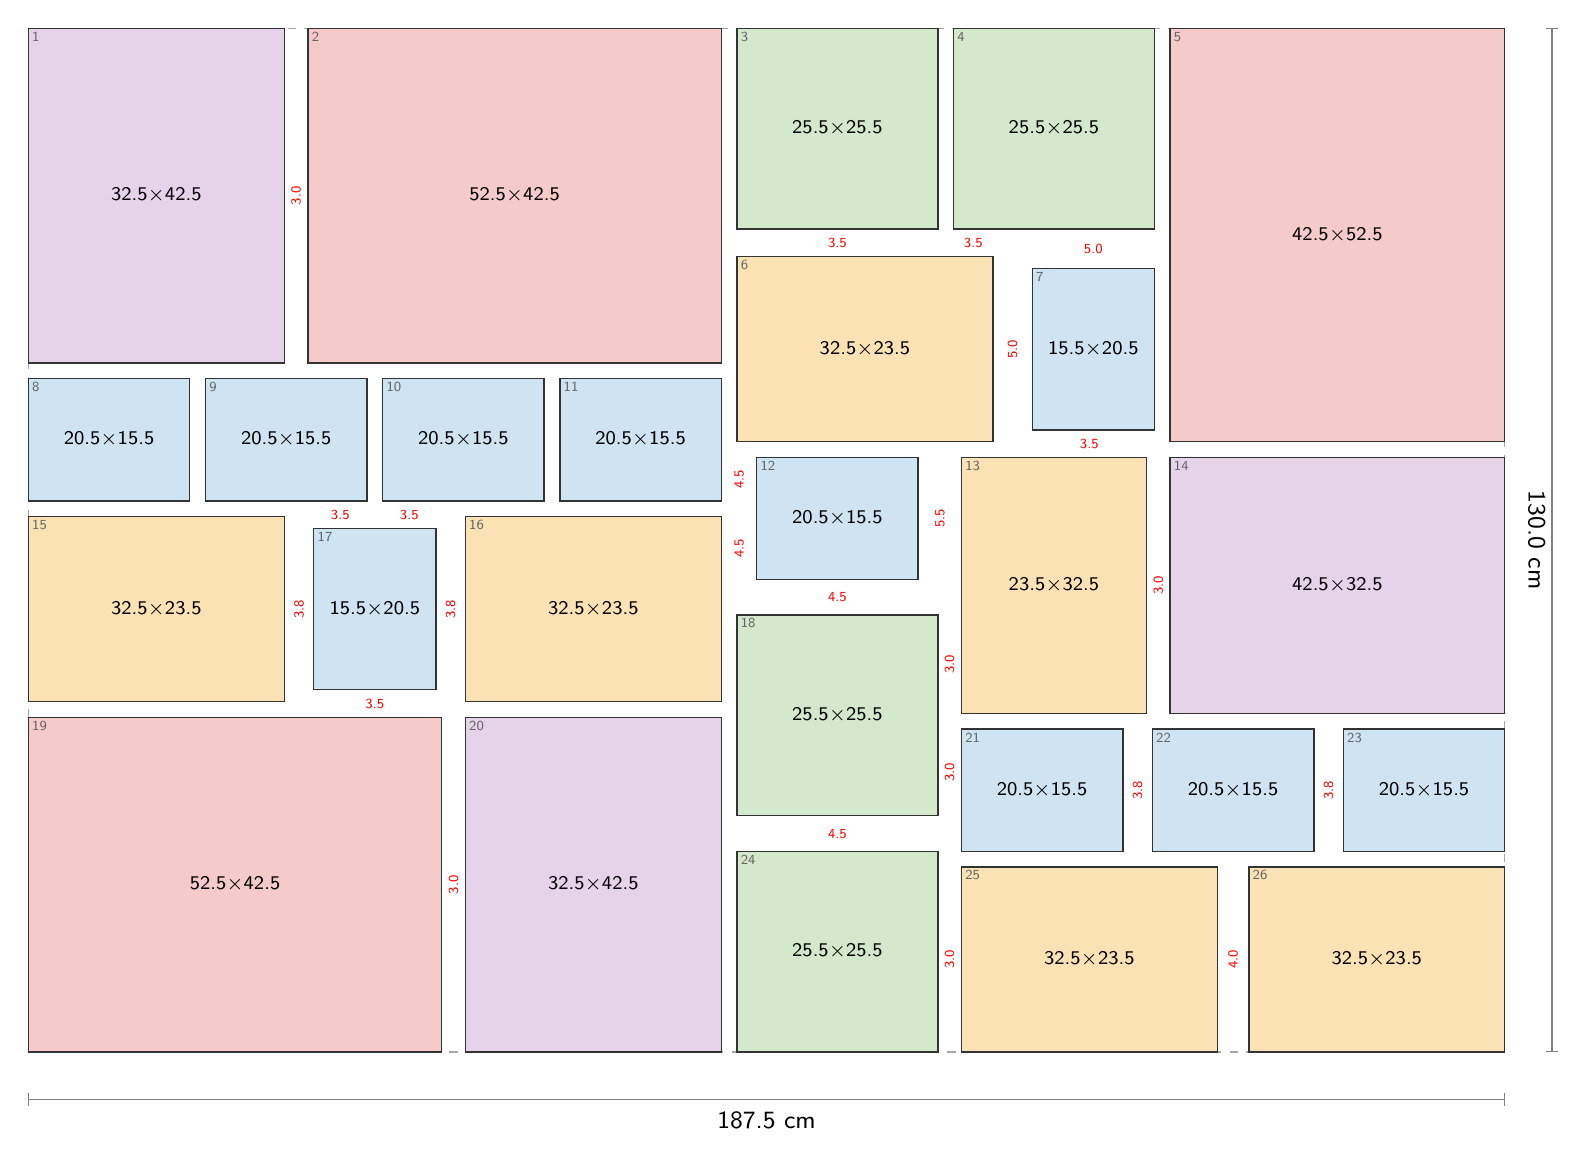
\begin{tikzpicture}[x=1mm, y=-1mm]
\draw[gray!70, dashed, line width=0.4pt] (0,0) rectangle (187.50,130.00);
\filldraw[fill=ft3, draw=black!80, line width=0.5pt] (0.00,0.00) rectangle (32.50,42.50);
\node[align=center, inner sep=0pt] at (16.25,21.25) {\scriptsize 32.5$\times$42.5};
\node[anchor=north west, inner sep=1.2pt, font=\tiny, text=black!60] at (0.00,0.00) {1};
\filldraw[fill=ft4, draw=black!80, line width=0.5pt] (35.50,0.00) rectangle (88.00,42.50);
\node[align=center, inner sep=0pt] at (61.75,21.25) {\scriptsize 52.5$\times$42.5};
\node[anchor=north west, inner sep=1.2pt, font=\tiny, text=black!60] at (35.50,0.00) {2};
\filldraw[fill=ft2, draw=black!80, line width=0.5pt] (90.00,0.00) rectangle (115.50,25.50);
\node[align=center, inner sep=0pt] at (102.75,12.75) {\scriptsize 25.5$\times$25.5};
\node[anchor=north west, inner sep=1.2pt, font=\tiny, text=black!60] at (90.00,0.00) {3};
\filldraw[fill=ft2, draw=black!80, line width=0.5pt] (117.50,0.00) rectangle (143.00,25.50);
\node[align=center, inner sep=0pt] at (130.25,12.75) {\scriptsize 25.5$\times$25.5};
\node[anchor=north west, inner sep=1.2pt, font=\tiny, text=black!60] at (117.50,0.00) {4};
\filldraw[fill=ft4, draw=black!80, line width=0.5pt] (145.00,0.00) rectangle (187.50,52.50);
\node[align=center, inner sep=0pt] at (166.25,26.25) {\scriptsize 42.5$\times$52.5};
\node[anchor=north west, inner sep=1.2pt, font=\tiny, text=black!60] at (145.00,0.00) {5};
\filldraw[fill=ft1, draw=black!80, line width=0.5pt] (90.00,29.00) rectangle (122.50,52.50);
\node[align=center, inner sep=0pt] at (106.25,40.75) {\scriptsize 32.5$\times$23.5};
\node[anchor=north west, inner sep=1.2pt, font=\tiny, text=black!60] at (90.00,29.00) {6};
\filldraw[fill=ft0, draw=black!80, line width=0.5pt] (127.50,30.50) rectangle (143.00,51.00);
\node[align=center, inner sep=0pt] at (135.25,40.75) {\scriptsize 15.5$\times$20.5};
\node[anchor=north west, inner sep=1.2pt, font=\tiny, text=black!60] at (127.50,30.50) {7};
\filldraw[fill=ft0, draw=black!80, line width=0.5pt] (0.00,44.50) rectangle (20.50,60.00);
\node[align=center, inner sep=0pt] at (10.25,52.25) {\scriptsize 20.5$\times$15.5};
\node[anchor=north west, inner sep=1.2pt, font=\tiny, text=black!60] at (0.00,44.50) {8};
\filldraw[fill=ft0, draw=black!80, line width=0.5pt] (22.50,44.50) rectangle (43.00,60.00);
\node[align=center, inner sep=0pt] at (32.75,52.25) {\scriptsize 20.5$\times$15.5};
\node[anchor=north west, inner sep=1.2pt, font=\tiny, text=black!60] at (22.50,44.50) {9};
\filldraw[fill=ft0, draw=black!80, line width=0.5pt] (45.00,44.50) rectangle (65.50,60.00);
\node[align=center, inner sep=0pt] at (55.25,52.25) {\scriptsize 20.5$\times$15.5};
\node[anchor=north west, inner sep=1.2pt, font=\tiny, text=black!60] at (45.00,44.50) {10};
\filldraw[fill=ft0, draw=black!80, line width=0.5pt] (67.50,44.50) rectangle (88.00,60.00);
\node[align=center, inner sep=0pt] at (77.75,52.25) {\scriptsize 20.5$\times$15.5};
\node[anchor=north west, inner sep=1.2pt, font=\tiny, text=black!60] at (67.50,44.50) {11};
\filldraw[fill=ft0, draw=black!80, line width=0.5pt] (92.50,54.50) rectangle (113.00,70.00);
\node[align=center, inner sep=0pt] at (102.75,62.25) {\scriptsize 20.5$\times$15.5};
\node[anchor=north west, inner sep=1.2pt, font=\tiny, text=black!60] at (92.50,54.50) {12};
\filldraw[fill=ft1, draw=black!80, line width=0.5pt] (118.50,54.50) rectangle (142.00,87.00);
\node[align=center, inner sep=0pt] at (130.25,70.75) {\scriptsize 23.5$\times$32.5};
\node[anchor=north west, inner sep=1.2pt, font=\tiny, text=black!60] at (118.50,54.50) {13};
\filldraw[fill=ft3, draw=black!80, line width=0.5pt] (145.00,54.50) rectangle (187.50,87.00);
\node[align=center, inner sep=0pt] at (166.25,70.75) {\scriptsize 42.5$\times$32.5};
\node[anchor=north west, inner sep=1.2pt, font=\tiny, text=black!60] at (145.00,54.50) {14};
\filldraw[fill=ft1, draw=black!80, line width=0.5pt] (0.00,62.00) rectangle (32.50,85.50);
\node[align=center, inner sep=0pt] at (16.25,73.75) {\scriptsize 32.5$\times$23.5};
\node[anchor=north west, inner sep=1.2pt, font=\tiny, text=black!60] at (0.00,62.00) {15};
\filldraw[fill=ft1, draw=black!80, line width=0.5pt] (55.50,62.00) rectangle (88.00,85.50);
\node[align=center, inner sep=0pt] at (71.75,73.75) {\scriptsize 32.5$\times$23.5};
\node[anchor=north west, inner sep=1.2pt, font=\tiny, text=black!60] at (55.50,62.00) {16};
\filldraw[fill=ft0, draw=black!80, line width=0.5pt] (36.25,63.50) rectangle (51.75,84.00);
\node[align=center, inner sep=0pt] at (44.00,73.75) {\scriptsize 15.5$\times$20.5};
\node[anchor=north west, inner sep=1.2pt, font=\tiny, text=black!60] at (36.25,63.50) {17};
\filldraw[fill=ft2, draw=black!80, line width=0.5pt] (90.00,74.50) rectangle (115.50,100.00);
\node[align=center, inner sep=0pt] at (102.75,87.25) {\scriptsize 25.5$\times$25.5};
\node[anchor=north west, inner sep=1.2pt, font=\tiny, text=black!60] at (90.00,74.50) {18};
\filldraw[fill=ft4, draw=black!80, line width=0.5pt] (0.00,87.50) rectangle (52.50,130.00);
\node[align=center, inner sep=0pt] at (26.25,108.75) {\scriptsize 52.5$\times$42.5};
\node[anchor=north west, inner sep=1.2pt, font=\tiny, text=black!60] at (0.00,87.50) {19};
\filldraw[fill=ft3, draw=black!80, line width=0.5pt] (55.50,87.50) rectangle (88.00,130.00);
\node[align=center, inner sep=0pt] at (71.75,108.75) {\scriptsize 32.5$\times$42.5};
\node[anchor=north west, inner sep=1.2pt, font=\tiny, text=black!60] at (55.50,87.50) {20};
\filldraw[fill=ft0, draw=black!80, line width=0.5pt] (118.50,89.00) rectangle (139.00,104.50);
\node[align=center, inner sep=0pt] at (128.75,96.75) {\scriptsize 20.5$\times$15.5};
\node[anchor=north west, inner sep=1.2pt, font=\tiny, text=black!60] at (118.50,89.00) {21};
\filldraw[fill=ft0, draw=black!80, line width=0.5pt] (142.75,89.00) rectangle (163.25,104.50);
\node[align=center, inner sep=0pt] at (153.00,96.75) {\scriptsize 20.5$\times$15.5};
\node[anchor=north west, inner sep=1.2pt, font=\tiny, text=black!60] at (142.75,89.00) {22};
\filldraw[fill=ft0, draw=black!80, line width=0.5pt] (167.00,89.00) rectangle (187.50,104.50);
\node[align=center, inner sep=0pt] at (177.25,96.75) {\scriptsize 20.5$\times$15.5};
\node[anchor=north west, inner sep=1.2pt, font=\tiny, text=black!60] at (167.00,89.00) {23};
\filldraw[fill=ft2, draw=black!80, line width=0.5pt] (90.00,104.50) rectangle (115.50,130.00);
\node[align=center, inner sep=0pt] at (102.75,117.25) {\scriptsize 25.5$\times$25.5};
\node[anchor=north west, inner sep=1.2pt, font=\tiny, text=black!60] at (90.00,104.50) {24};
\filldraw[fill=ft1, draw=black!80, line width=0.5pt] (118.50,106.50) rectangle (151.00,130.00);
\node[align=center, inner sep=0pt] at (134.75,118.25) {\scriptsize 32.5$\times$23.5};
\node[anchor=north west, inner sep=1.2pt, font=\tiny, text=black!60] at (118.50,106.50) {25};
\filldraw[fill=ft1, draw=black!80, line width=0.5pt] (155.00,106.50) rectangle (187.50,130.00);
\node[align=center, inner sep=0pt] at (171.25,118.25) {\scriptsize 32.5$\times$23.5};
\node[anchor=north west, inner sep=1.2pt, font=\tiny, text=black!60] at (155.00,106.50) {26};
\node[font=\tiny, text=red, fill=white, inner sep=0.3pt, rotate=90] at (34.00,21.25) {3.0};
\node[font=\tiny, text=red, fill=white, inner sep=0.3pt] at (102.75,27.25) {3.5};
\node[font=\tiny, text=red, fill=white, inner sep=0.3pt] at (120.00,27.25) {3.5};
\node[font=\tiny, text=red, fill=white, inner sep=0.3pt] at (135.25,28.00) {5.0};
\node[font=\tiny, text=red, fill=white, inner sep=0.3pt, rotate=90] at (125.00,40.75) {5.0};
\node[font=\tiny, text=red, fill=white, inner sep=0.3pt] at (134.75,52.75) {3.5};
\node[font=\tiny, text=red, fill=white, inner sep=0.3pt] at (39.62,61.75) {3.5};
\node[font=\tiny, text=red, fill=white, inner sep=0.3pt] at (48.38,61.75) {3.5};
\node[font=\tiny, text=red, fill=white, inner sep=0.3pt, rotate=90] at (90.25,57.25) {4.5};
\node[font=\tiny, text=red, fill=white, inner sep=0.3pt, rotate=90] at (115.75,62.25) {5.5};
\node[font=\tiny, text=red, fill=white, inner sep=0.3pt] at (102.75,72.25) {4.5};
\node[font=\tiny, text=red, fill=white, inner sep=0.3pt, rotate=90] at (143.50,70.75) {3.0};
\node[font=\tiny, text=red, fill=white, inner sep=0.3pt, rotate=90] at (34.38,73.75) {3.8};
\node[font=\tiny, text=red, fill=white, inner sep=0.3pt, rotate=90] at (90.25,66.00) {4.5};
\node[font=\tiny, text=red, fill=white, inner sep=0.3pt, rotate=90] at (53.62,73.75) {3.8};
\node[font=\tiny, text=red, fill=white, inner sep=0.3pt] at (44.00,85.75) {3.5};
\node[font=\tiny, text=red, fill=white, inner sep=0.3pt, rotate=90] at (117.00,80.75) {3.0};
\node[font=\tiny, text=red, fill=white, inner sep=0.3pt, rotate=90] at (117.00,94.50) {3.0};
\node[font=\tiny, text=red, fill=white, inner sep=0.3pt] at (102.75,102.25) {4.5};
\node[font=\tiny, text=red, fill=white, inner sep=0.3pt, rotate=90] at (54.00,108.75) {3.0};
\node[font=\tiny, text=red, fill=white, inner sep=0.3pt, rotate=90] at (140.88,96.75) {3.8};
\node[font=\tiny, text=red, fill=white, inner sep=0.3pt, rotate=90] at (165.12,96.75) {3.8};
\node[font=\tiny, text=red, fill=white, inner sep=0.3pt, rotate=90] at (117.00,118.25) {3.0};
\node[font=\tiny, text=red, fill=white, inner sep=0.3pt, rotate=90] at (153.00,118.25) {4.0};
\draw[Bar-Bar, gray] (0,136.00) -- (187.50,136.00) node[midway, below=1pt, font=\small, text=black] {187.5 cm};
\draw[Bar-Bar, gray] (193.50,0) -- (193.50,130.00) node[midway, right=1pt, font=\small, text=black, rotate=-90, anchor=north] {130.0 cm};
\end{tikzpicture}\\[4pt]
{\scriptsize Scale 1:10 (1 mm = 1 cm). Red numbers mark gaps that deviate from the nominal gap by more than 0.25 cm. Small grey numbers index the coordinate table.}
\end{minipage}\hfill
\begin{minipage}[t]{0.25\textwidth}\vspace{0pt}
\small
\begin{tabular}{@{}l l@{}}
\toprule
Outer size & 187.5 $\times$ 130.0 cm \\
Nominal gap & 2 cm \\
Actual gaps & 2.0 -- 5.5 cm \\
Max.\ deviation & 3.5 cm \\
Mean deviation & 0.78 cm \\
Border notches & bottom 4 cm \\
Corners filled & 4 / 4 \\
Frames used & 26 of 28 \\
\bottomrule
\end{tabular}

\vspace{8pt}
\scriptsize
\begin{tabular}{@{}c l l r r@{}}
\toprule
 & outer w $\times$ h (cm) & & used & have \\
\midrule
\tikz[baseline=-0.6ex]\fill[ft0,draw=black!60] (0,0) rectangle (1.2ex,1.2ex); & 20.5$\times$15.5 & L & 8 & 9 \\
\tikz[baseline=-0.6ex]\fill[ft0,draw=black!60] (0,0) rectangle (1.2ex,1.2ex); & 15.5$\times$20.5 & P & 2 & 2 \\
\tikz[baseline=-0.6ex]\fill[ft3,draw=black!60] (0,0) rectangle (1.2ex,1.2ex); & 32.5$\times$42.5 & P & 2 & 2 \\
\tikz[baseline=-0.6ex]\fill[ft3,draw=black!60] (0,0) rectangle (1.2ex,1.2ex); & 42.5$\times$32.5 & L & 1 & 1 \\
\tikz[baseline=-0.6ex]\fill[ft1,draw=black!60] (0,0) rectangle (1.2ex,1.2ex); & 32.5$\times$23.5 & L & 5 & 5 \\
\tikz[baseline=-0.6ex]\fill[ft1,draw=black!60] (0,0) rectangle (1.2ex,1.2ex); & 23.5$\times$32.5 & P & 1 & 1 \\
\tikz[baseline=-0.6ex]\fill[ft2,draw=black!60] (0,0) rectangle (1.2ex,1.2ex); & 25.5$\times$25.5 &  & 4 & 5 \\
\tikz[baseline=-0.6ex]\fill[ft4,draw=black!60] (0,0) rectangle (1.2ex,1.2ex); & 42.5$\times$52.5 & P & 1 & 1 \\
\tikz[baseline=-0.6ex]\fill[ft4,draw=black!60] (0,0) rectangle (1.2ex,1.2ex); & 52.5$\times$42.5 & L & 2 & 2 \\
\bottomrule
\end{tabular}

\vspace{8pt}
{\bfseries Positions} (top-left corner, cm)\\[2pt]
\tiny
\begin{tabular}{@{}r l r r@{}}
\toprule
\# & frame w $\times$ h & x & y \\
\midrule
1 & 32.5 $\times$ 42.5 & 0.0 & 0.0 \\
2 & 52.5 $\times$ 42.5 & 35.5 & 0.0 \\
3 & 25.5 $\times$ 25.5 & 90.0 & 0.0 \\
4 & 25.5 $\times$ 25.5 & 117.5 & 0.0 \\
5 & 42.5 $\times$ 52.5 & 145.0 & 0.0 \\
6 & 32.5 $\times$ 23.5 & 90.0 & 29.0 \\
7 & 15.5 $\times$ 20.5 & 127.5 & 30.5 \\
8 & 20.5 $\times$ 15.5 & 0.0 & 44.5 \\
9 & 20.5 $\times$ 15.5 & 22.5 & 44.5 \\
10 & 20.5 $\times$ 15.5 & 45.0 & 44.5 \\
11 & 20.5 $\times$ 15.5 & 67.5 & 44.5 \\
12 & 20.5 $\times$ 15.5 & 92.5 & 54.5 \\
13 & 23.5 $\times$ 32.5 & 118.5 & 54.5 \\
14 & 42.5 $\times$ 32.5 & 145.0 & 54.5 \\
15 & 32.5 $\times$ 23.5 & 0.0 & 62.0 \\
16 & 32.5 $\times$ 23.5 & 55.5 & 62.0 \\
17 & 15.5 $\times$ 20.5 & 36.2 & 63.5 \\
18 & 25.5 $\times$ 25.5 & 90.0 & 74.5 \\
19 & 52.5 $\times$ 42.5 & 0.0 & 87.5 \\
20 & 32.5 $\times$ 42.5 & 55.5 & 87.5 \\
21 & 20.5 $\times$ 15.5 & 118.5 & 89.0 \\
22 & 20.5 $\times$ 15.5 & 142.8 & 89.0 \\
23 & 20.5 $\times$ 15.5 & 167.0 & 89.0 \\
24 & 25.5 $\times$ 25.5 & 90.0 & 104.5 \\
25 & 32.5 $\times$ 23.5 & 118.5 & 106.5 \\
26 & 32.5 $\times$ 23.5 & 155.0 & 106.5 \\
\bottomrule
\end{tabular}
\end{minipage}
\clearpage

\begin{minipage}[t]{0.74\textwidth}\vspace{0pt}
{\LARGE\bfseries Layout 16}\hspace{1.5em}{\large 180.0 $\times$ 114.5 cm \quad gap 2 cm \quad 25 frames}\\[8pt]
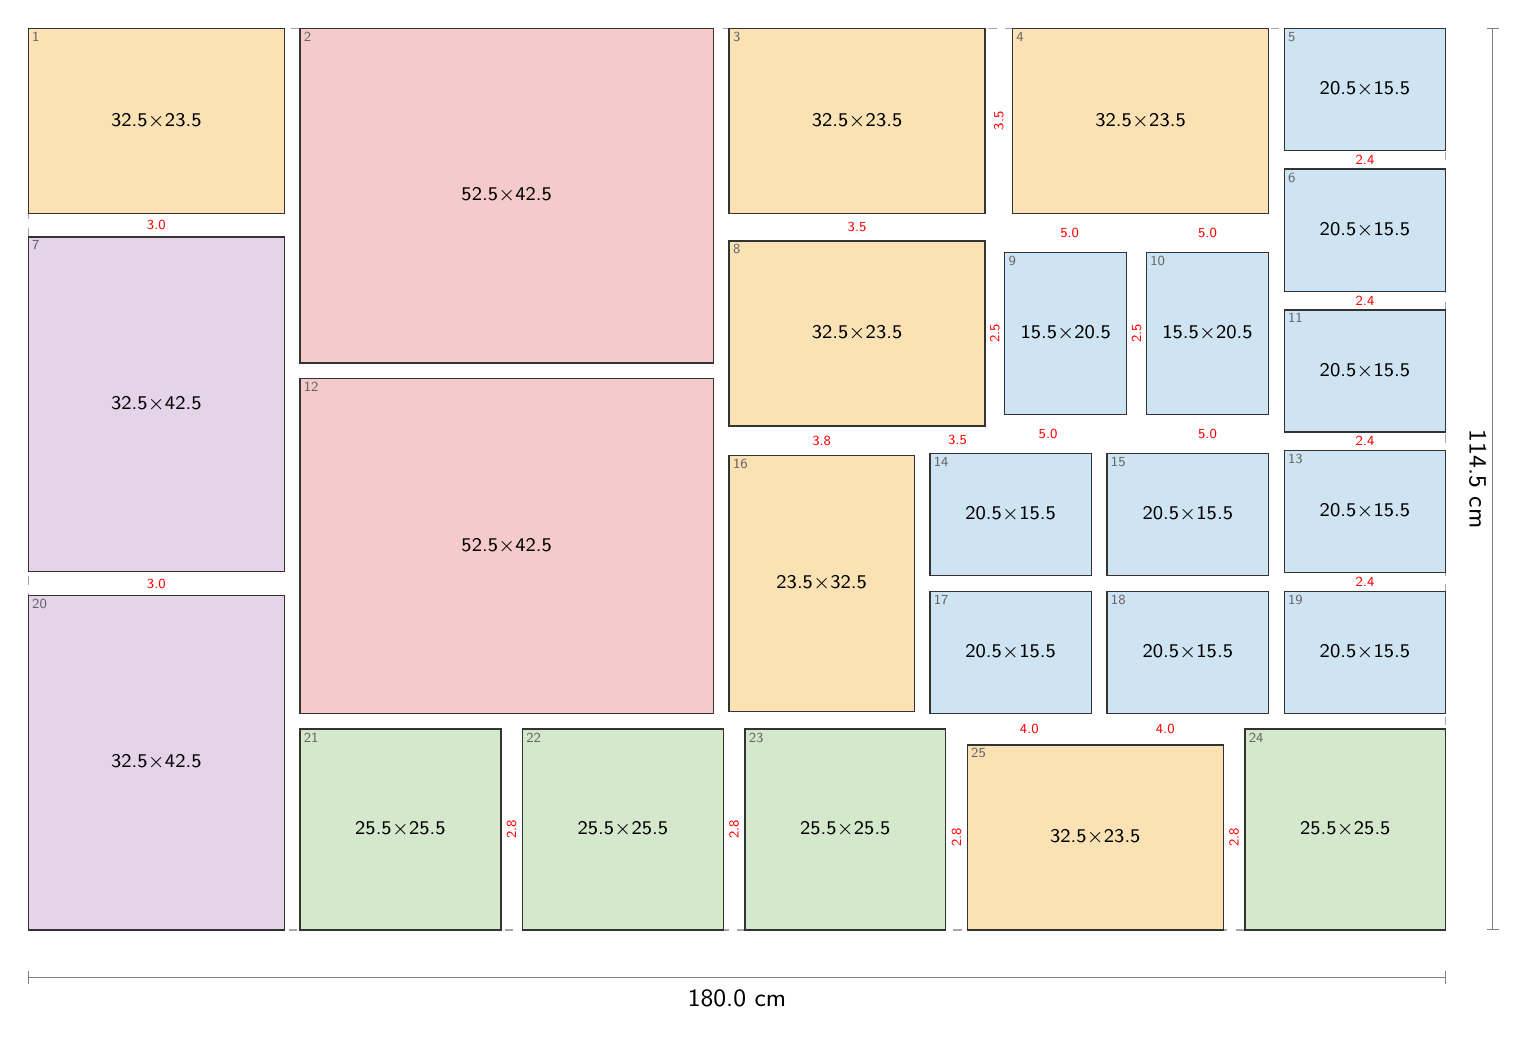
\begin{tikzpicture}[x=1mm, y=-1mm]
\draw[gray!70, dashed, line width=0.4pt] (0,0) rectangle (180.00,114.50);
\filldraw[fill=ft1, draw=black!80, line width=0.5pt] (0.00,0.00) rectangle (32.50,23.50);
\node[align=center, inner sep=0pt] at (16.25,11.75) {\scriptsize 32.5$\times$23.5};
\node[anchor=north west, inner sep=1.2pt, font=\tiny, text=black!60] at (0.00,0.00) {1};
\filldraw[fill=ft4, draw=black!80, line width=0.5pt] (34.50,0.00) rectangle (87.00,42.50);
\node[align=center, inner sep=0pt] at (60.75,21.25) {\scriptsize 52.5$\times$42.5};
\node[anchor=north west, inner sep=1.2pt, font=\tiny, text=black!60] at (34.50,0.00) {2};
\filldraw[fill=ft1, draw=black!80, line width=0.5pt] (89.00,0.00) rectangle (121.50,23.50);
\node[align=center, inner sep=0pt] at (105.25,11.75) {\scriptsize 32.5$\times$23.5};
\node[anchor=north west, inner sep=1.2pt, font=\tiny, text=black!60] at (89.00,0.00) {3};
\filldraw[fill=ft1, draw=black!80, line width=0.5pt] (125.00,0.00) rectangle (157.50,23.50);
\node[align=center, inner sep=0pt] at (141.25,11.75) {\scriptsize 32.5$\times$23.5};
\node[anchor=north west, inner sep=1.2pt, font=\tiny, text=black!60] at (125.00,0.00) {4};
\filldraw[fill=ft0, draw=black!80, line width=0.5pt] (159.50,0.00) rectangle (180.00,15.50);
\node[align=center, inner sep=0pt] at (169.75,7.75) {\scriptsize 20.5$\times$15.5};
\node[anchor=north west, inner sep=1.2pt, font=\tiny, text=black!60] at (159.50,0.00) {5};
\filldraw[fill=ft0, draw=black!80, line width=0.5pt] (159.50,17.88) rectangle (180.00,33.38);
\node[align=center, inner sep=0pt] at (169.75,25.62) {\scriptsize 20.5$\times$15.5};
\node[anchor=north west, inner sep=1.2pt, font=\tiny, text=black!60] at (159.50,17.88) {6};
\filldraw[fill=ft3, draw=black!80, line width=0.5pt] (0.00,26.50) rectangle (32.50,69.00);
\node[align=center, inner sep=0pt] at (16.25,47.75) {\scriptsize 32.5$\times$42.5};
\node[anchor=north west, inner sep=1.2pt, font=\tiny, text=black!60] at (0.00,26.50) {7};
\filldraw[fill=ft1, draw=black!80, line width=0.5pt] (89.00,27.00) rectangle (121.50,50.50);
\node[align=center, inner sep=0pt] at (105.25,38.75) {\scriptsize 32.5$\times$23.5};
\node[anchor=north west, inner sep=1.2pt, font=\tiny, text=black!60] at (89.00,27.00) {8};
\filldraw[fill=ft0, draw=black!80, line width=0.5pt] (124.00,28.50) rectangle (139.50,49.00);
\node[align=center, inner sep=0pt] at (131.75,38.75) {\scriptsize 15.5$\times$20.5};
\node[anchor=north west, inner sep=1.2pt, font=\tiny, text=black!60] at (124.00,28.50) {9};
\filldraw[fill=ft0, draw=black!80, line width=0.5pt] (142.00,28.50) rectangle (157.50,49.00);
\node[align=center, inner sep=0pt] at (149.75,38.75) {\scriptsize 15.5$\times$20.5};
\node[anchor=north west, inner sep=1.2pt, font=\tiny, text=black!60] at (142.00,28.50) {10};
\filldraw[fill=ft0, draw=black!80, line width=0.5pt] (159.50,35.75) rectangle (180.00,51.25);
\node[align=center, inner sep=0pt] at (169.75,43.50) {\scriptsize 20.5$\times$15.5};
\node[anchor=north west, inner sep=1.2pt, font=\tiny, text=black!60] at (159.50,35.75) {11};
\filldraw[fill=ft4, draw=black!80, line width=0.5pt] (34.50,44.50) rectangle (87.00,87.00);
\node[align=center, inner sep=0pt] at (60.75,65.75) {\scriptsize 52.5$\times$42.5};
\node[anchor=north west, inner sep=1.2pt, font=\tiny, text=black!60] at (34.50,44.50) {12};
\filldraw[fill=ft0, draw=black!80, line width=0.5pt] (159.50,53.62) rectangle (180.00,69.12);
\node[align=center, inner sep=0pt] at (169.75,61.38) {\scriptsize 20.5$\times$15.5};
\node[anchor=north west, inner sep=1.2pt, font=\tiny, text=black!60] at (159.50,53.62) {13};
\filldraw[fill=ft0, draw=black!80, line width=0.5pt] (114.50,54.00) rectangle (135.00,69.50);
\node[align=center, inner sep=0pt] at (124.75,61.75) {\scriptsize 20.5$\times$15.5};
\node[anchor=north west, inner sep=1.2pt, font=\tiny, text=black!60] at (114.50,54.00) {14};
\filldraw[fill=ft0, draw=black!80, line width=0.5pt] (137.00,54.00) rectangle (157.50,69.50);
\node[align=center, inner sep=0pt] at (147.25,61.75) {\scriptsize 20.5$\times$15.5};
\node[anchor=north west, inner sep=1.2pt, font=\tiny, text=black!60] at (137.00,54.00) {15};
\filldraw[fill=ft1, draw=black!80, line width=0.5pt] (89.00,54.25) rectangle (112.50,86.75);
\node[align=center, inner sep=0pt] at (100.75,70.50) {\scriptsize 23.5$\times$32.5};
\node[anchor=north west, inner sep=1.2pt, font=\tiny, text=black!60] at (89.00,54.25) {16};
\filldraw[fill=ft0, draw=black!80, line width=0.5pt] (114.50,71.50) rectangle (135.00,87.00);
\node[align=center, inner sep=0pt] at (124.75,79.25) {\scriptsize 20.5$\times$15.5};
\node[anchor=north west, inner sep=1.2pt, font=\tiny, text=black!60] at (114.50,71.50) {17};
\filldraw[fill=ft0, draw=black!80, line width=0.5pt] (137.00,71.50) rectangle (157.50,87.00);
\node[align=center, inner sep=0pt] at (147.25,79.25) {\scriptsize 20.5$\times$15.5};
\node[anchor=north west, inner sep=1.2pt, font=\tiny, text=black!60] at (137.00,71.50) {18};
\filldraw[fill=ft0, draw=black!80, line width=0.5pt] (159.50,71.50) rectangle (180.00,87.00);
\node[align=center, inner sep=0pt] at (169.75,79.25) {\scriptsize 20.5$\times$15.5};
\node[anchor=north west, inner sep=1.2pt, font=\tiny, text=black!60] at (159.50,71.50) {19};
\filldraw[fill=ft3, draw=black!80, line width=0.5pt] (0.00,72.00) rectangle (32.50,114.50);
\node[align=center, inner sep=0pt] at (16.25,93.25) {\scriptsize 32.5$\times$42.5};
\node[anchor=north west, inner sep=1.2pt, font=\tiny, text=black!60] at (0.00,72.00) {20};
\filldraw[fill=ft2, draw=black!80, line width=0.5pt] (34.50,89.00) rectangle (60.00,114.50);
\node[align=center, inner sep=0pt] at (47.25,101.75) {\scriptsize 25.5$\times$25.5};
\node[anchor=north west, inner sep=1.2pt, font=\tiny, text=black!60] at (34.50,89.00) {21};
\filldraw[fill=ft2, draw=black!80, line width=0.5pt] (62.75,89.00) rectangle (88.25,114.50);
\node[align=center, inner sep=0pt] at (75.50,101.75) {\scriptsize 25.5$\times$25.5};
\node[anchor=north west, inner sep=1.2pt, font=\tiny, text=black!60] at (62.75,89.00) {22};
\filldraw[fill=ft2, draw=black!80, line width=0.5pt] (91.00,89.00) rectangle (116.50,114.50);
\node[align=center, inner sep=0pt] at (103.75,101.75) {\scriptsize 25.5$\times$25.5};
\node[anchor=north west, inner sep=1.2pt, font=\tiny, text=black!60] at (91.00,89.00) {23};
\filldraw[fill=ft2, draw=black!80, line width=0.5pt] (154.50,89.00) rectangle (180.00,114.50);
\node[align=center, inner sep=0pt] at (167.25,101.75) {\scriptsize 25.5$\times$25.5};
\node[anchor=north west, inner sep=1.2pt, font=\tiny, text=black!60] at (154.50,89.00) {24};
\filldraw[fill=ft1, draw=black!80, line width=0.5pt] (119.25,91.00) rectangle (151.75,114.50);
\node[align=center, inner sep=0pt] at (135.50,102.75) {\scriptsize 32.5$\times$23.5};
\node[anchor=north west, inner sep=1.2pt, font=\tiny, text=black!60] at (119.25,91.00) {25};
\node[font=\tiny, text=red, fill=white, inner sep=0.3pt] at (16.25,25.00) {3.0};
\node[font=\tiny, text=red, fill=white, inner sep=0.3pt, rotate=90] at (123.25,11.75) {3.5};
\node[font=\tiny, text=red, fill=white, inner sep=0.3pt] at (105.25,25.25) {3.5};
\node[font=\tiny, text=red, fill=white, inner sep=0.3pt] at (132.25,26.00) {5.0};
\node[font=\tiny, text=red, fill=white, inner sep=0.3pt] at (149.75,26.00) {5.0};
\node[font=\tiny, text=red, fill=white, inner sep=0.3pt] at (169.75,16.69) {2.4};
\node[font=\tiny, text=red, fill=white, inner sep=0.3pt] at (169.75,34.56) {2.4};
\node[font=\tiny, text=red, fill=white, inner sep=0.3pt] at (16.25,70.50) {3.0};
\node[font=\tiny, text=red, fill=white, inner sep=0.3pt, rotate=90] at (122.75,38.75) {2.5};
\node[font=\tiny, text=red, fill=white, inner sep=0.3pt] at (118.00,52.25) {3.5};
\node[font=\tiny, text=red, fill=white, inner sep=0.3pt] at (100.75,52.38) {3.8};
\node[font=\tiny, text=red, fill=white, inner sep=0.3pt, rotate=90] at (140.75,38.75) {2.5};
\node[font=\tiny, text=red, fill=white, inner sep=0.3pt] at (129.50,51.50) {5.0};
\node[font=\tiny, text=red, fill=white, inner sep=0.3pt] at (149.75,51.50) {5.0};
\node[font=\tiny, text=red, fill=white, inner sep=0.3pt] at (169.75,52.44) {2.4};
\node[font=\tiny, text=red, fill=white, inner sep=0.3pt] at (169.75,70.31) {2.4};
\node[font=\tiny, text=red, fill=white, inner sep=0.3pt] at (127.12,89.00) {4.0};
\node[font=\tiny, text=red, fill=white, inner sep=0.3pt] at (144.38,89.00) {4.0};
\node[font=\tiny, text=red, fill=white, inner sep=0.3pt, rotate=90] at (61.38,101.75) {2.8};
\node[font=\tiny, text=red, fill=white, inner sep=0.3pt, rotate=90] at (89.62,101.75) {2.8};
\node[font=\tiny, text=red, fill=white, inner sep=0.3pt, rotate=90] at (117.88,102.75) {2.8};
\node[font=\tiny, text=red, fill=white, inner sep=0.3pt, rotate=90] at (153.12,102.75) {2.8};
\draw[Bar-Bar, gray] (0,120.50) -- (180.00,120.50) node[midway, below=1pt, font=\small, text=black] {180.0 cm};
\draw[Bar-Bar, gray] (186.00,0) -- (186.00,114.50) node[midway, right=1pt, font=\small, text=black, rotate=-90, anchor=north] {114.5 cm};
\end{tikzpicture}\\[4pt]
{\scriptsize Scale 1:10 (1 mm = 1 cm). Red numbers mark gaps that deviate from the nominal gap by more than 0.25 cm. Small grey numbers index the coordinate table.}
\end{minipage}\hfill
\begin{minipage}[t]{0.25\textwidth}\vspace{0pt}
\small
\begin{tabular}{@{}l l@{}}
\toprule
Outer size & 180.0 $\times$ 114.5 cm \\
Nominal gap & 2 cm \\
Actual gaps & 2.0 -- 5.0 cm \\
Max.\ deviation & 3.0 cm \\
Mean deviation & 0.64 cm \\
Border notches & top 4 cm \\
Corners filled & 4 / 4 \\
Frames used & 25 of 28 \\
\bottomrule
\end{tabular}

\vspace{8pt}
\scriptsize
\begin{tabular}{@{}c l l r r@{}}
\toprule
 & outer w $\times$ h (cm) & & used & have \\
\midrule
\tikz[baseline=-0.6ex]\fill[ft0,draw=black!60] (0,0) rectangle (1.2ex,1.2ex); & 20.5$\times$15.5 & L & 9 & 9 \\
\tikz[baseline=-0.6ex]\fill[ft0,draw=black!60] (0,0) rectangle (1.2ex,1.2ex); & 15.5$\times$20.5 & P & 2 & 2 \\
\tikz[baseline=-0.6ex]\fill[ft3,draw=black!60] (0,0) rectangle (1.2ex,1.2ex); & 32.5$\times$42.5 & P & 2 & 2 \\
\tikz[baseline=-0.6ex]\fill[ft3,draw=black!60] (0,0) rectangle (1.2ex,1.2ex); & 42.5$\times$32.5 & L & 0 & 1 \\
\tikz[baseline=-0.6ex]\fill[ft1,draw=black!60] (0,0) rectangle (1.2ex,1.2ex); & 32.5$\times$23.5 & L & 5 & 5 \\
\tikz[baseline=-0.6ex]\fill[ft1,draw=black!60] (0,0) rectangle (1.2ex,1.2ex); & 23.5$\times$32.5 & P & 1 & 1 \\
\tikz[baseline=-0.6ex]\fill[ft2,draw=black!60] (0,0) rectangle (1.2ex,1.2ex); & 25.5$\times$25.5 &  & 4 & 5 \\
\tikz[baseline=-0.6ex]\fill[ft4,draw=black!60] (0,0) rectangle (1.2ex,1.2ex); & 42.5$\times$52.5 & P & 0 & 1 \\
\tikz[baseline=-0.6ex]\fill[ft4,draw=black!60] (0,0) rectangle (1.2ex,1.2ex); & 52.5$\times$42.5 & L & 2 & 2 \\
\bottomrule
\end{tabular}

\vspace{8pt}
{\bfseries Positions} (top-left corner, cm)\\[2pt]
\tiny
\begin{tabular}{@{}r l r r@{}}
\toprule
\# & frame w $\times$ h & x & y \\
\midrule
1 & 32.5 $\times$ 23.5 & 0.0 & 0.0 \\
2 & 52.5 $\times$ 42.5 & 34.5 & 0.0 \\
3 & 32.5 $\times$ 23.5 & 89.0 & 0.0 \\
4 & 32.5 $\times$ 23.5 & 125.0 & 0.0 \\
5 & 20.5 $\times$ 15.5 & 159.5 & 0.0 \\
6 & 20.5 $\times$ 15.5 & 159.5 & 17.9 \\
7 & 32.5 $\times$ 42.5 & 0.0 & 26.5 \\
8 & 32.5 $\times$ 23.5 & 89.0 & 27.0 \\
9 & 15.5 $\times$ 20.5 & 124.0 & 28.5 \\
10 & 15.5 $\times$ 20.5 & 142.0 & 28.5 \\
11 & 20.5 $\times$ 15.5 & 159.5 & 35.8 \\
12 & 52.5 $\times$ 42.5 & 34.5 & 44.5 \\
13 & 20.5 $\times$ 15.5 & 159.5 & 53.6 \\
14 & 20.5 $\times$ 15.5 & 114.5 & 54.0 \\
15 & 20.5 $\times$ 15.5 & 137.0 & 54.0 \\
16 & 23.5 $\times$ 32.5 & 89.0 & 54.2 \\
17 & 20.5 $\times$ 15.5 & 114.5 & 71.5 \\
18 & 20.5 $\times$ 15.5 & 137.0 & 71.5 \\
19 & 20.5 $\times$ 15.5 & 159.5 & 71.5 \\
20 & 32.5 $\times$ 42.5 & 0.0 & 72.0 \\
21 & 25.5 $\times$ 25.5 & 34.5 & 89.0 \\
22 & 25.5 $\times$ 25.5 & 62.8 & 89.0 \\
23 & 25.5 $\times$ 25.5 & 91.0 & 89.0 \\
24 & 25.5 $\times$ 25.5 & 154.5 & 89.0 \\
25 & 32.5 $\times$ 23.5 & 119.2 & 91.0 \\
\bottomrule
\end{tabular}
\end{minipage}
\clearpage

\end{document}
